\documentclass[11pt]{article}
\setlength{\parindent}{0pt}
\setlength{\parskip}{1em}

\usepackage{amsmath}
\usepackage{amsthm}
\usepackage{amssymb}
\usepackage{bbm}
\usepackage{authblk}
\usepackage{fancyhdr}
\usepackage{geometry}
\usepackage{hyperref}
\usepackage{mdwlist}
\usepackage{ragged2e}
\usepackage{titlesec}
\usepackage{verbatim}
\usepackage{xspace}
\usepackage{graphicx}
\usepackage{pgf}
\usepackage{tikz}
\usepackage{multicol}
\usetikzlibrary{arrows}
\usetikzlibrary{shapes.geometric}
\usepackage{float}
\usepackage[titles]{tocloft}
\usepackage{fancyvrb}
\fvset{samepage,fontsize=\small}

\pagestyle{fancy}
\fancyhf{}
\rhead{\footnotesize CC BY-SA 4.0}
\lhead{\footnotesize\raisebox{1.25pt}{\fontsize{7}{7}\textcopyright}\hspace{2pt}Zoom Video Communications, Inc.}
\lfoot{\footnotesize Zoom Cryptography Whitepaper}
\rfoot{\footnotesize Page \thepage}

%tilepage has no footer
\fancypagestyle{titlepage}{
\fancyhf{}
\rhead{\footnotesize CC BY-SA 4.0}
\lhead{\footnotesize\raisebox{1.25pt}{\fontsize{7}{7}\textcopyright}\hspace{2pt}Zoom Video Communications, Inc.}
\lfoot{$^*$Zoom is grateful for the collaboration and expertise of our co-authors, who appear here if they
contributed to any version of this whitepaper.}
}

\newcommand{\true}{\mathsf{true}}
\newcommand{\false}{\mathsf{false}}

\newcommand{\pk}{\mathit{pk}}
\newcommand{\sk}{\mathit{sk}}

\newcommand{\keygen}{\ensuremath{\mathsf{KeyGen}}}

\newcommand{\enc}{\ensuremath{\mathsf{Enc}}}
\newcommand{\dec}{\ensuremath{\mathsf{Dec}}}
\newcommand{\sign}{\ensuremath{\mathsf{Sign}}}
\newcommand{\verify}{\ensuremath{\mathsf{Verify}}}

\newcommand{\vk}{\mathit{vk}}

\newcommand{\eddsa}{EdDSA}
\newcommand{\ecdsa}{ECDSA}
\newcommand{\zoomsign}{Sign}
\newcommand{\cbox}{Box}

\newcommand{\vkeddsa}{\vk_{{\sf \eddsa}}}
\newcommand{\skeddsa}{\sk_{{\sf \eddsa}}}
\newcommand{\signatureeddsa}{{\sf Sig}_{{\sf \eddsa}}}
\newcommand{\eddsakeygen}{{\sf \eddsa}.\keygen}
\newcommand{\eddsasign}{{\sf \eddsa}.\sign}
\newcommand{\eddsaverify}{{\sf \eddsa}.\verify}
\newcommand{\errorSym}{{\sf error}}

\newcommand{\sig}{{\sf Sig}}

\newcommand{\vkecdsa}{\vk_{{\sf \ecdsa}}}
\newcommand{\skecdsa}{\sk_{{\sf \ecdsa}}}
\newcommand{\signatureecdsa}{{\sf Sig}_{{\sf \ecdsa}}}
\newcommand{\ecdsakeygen}{{\sf \ecdsa}.\keygen}
\newcommand{\ecdsasign}{{\sf \ecdsa}.\sign}
\newcommand{\ecdsaverify}{{\sf \ecdsa}.\verify}

\newcommand{\kyberkemenc}{{\sf Kyber}.\sf{KemEnc}}
\newcommand{\kyberkemdec}{{\sf Kyber}.\sf{KemDec}}

\newcommand{\vkzoomsign}{\vk}
\newcommand{\skzoomsign}{\sk}
\newcommand{\signaturezoomsign}{{\sf Sig}}
\newcommand{\zoomsignkeygen}{{\sf \zoomsign}.\keygen}
\newcommand{\zoomsignsign}{{\sf \zoomsign}.\sign}
\newcommand{\zoomsignverify}{{\sf \zoomsign}.\verify}

\newcommand{\genedkeypair}{{\sf GenCurve25519Keypair}}
\newcommand{\genfipskeypair}{{\sf GenFIPSKeypair}}
\newcommand{\pkfips}{\pk_{\sf FIPS}}
\newcommand{\skfips}{\sk_{\sf FIPS}}
\newcommand{\pked}{\pk_{\sf 25519}}
\newcommand{\sked}{\sk_{\sf 25519}}

\newcommand{\dhfunced}{{\sf DH}_{\sf 25519}}
\newcommand{\dhfuncfips}{{\sf DH}_{\sf FIPS}}

\newcommand{\kyber}{\sf Kyber}
\newcommand{\sfbox}{\sf Box}
\newcommand{\pkbox}{\pk_{{\sf \cbox}}}
\newcommand{\skbox}{\sk_{{\sf \cbox}}}
\newcommand{\pkkyber}{\pk_{{\sf Kyber}}}
\newcommand{\skkyber}{\sk_{{\sf Kyber}}}
\newcommand{\ciphertext}{C}
\newcommand{\cboxkeygen}{{\sf \cbox}.\keygen}
\newcommand{\cboxencrypt}{{\sf \cbox}.\enc}
\newcommand{\cboxdecrypt}{{\sf \cbox}.\dec}

\newcommand{\pkboxR}{\pkbox^{\sf R}}
\newcommand{\skboxS}{\skbox^{\sf S}}
\newcommand{\pkkyberR}{\pkkyber^{\sf R}}
\newcommand{\skkyberS}{\skkyber^{\sf S}}
\newcommand{\pkedR}{\pked^{\sf R}}
\newcommand{\skedS}{\sked^{\sf S}}
\newcommand{\pkfipsR}{\pkfips^{\sf R}}
\newcommand{\skfipsS}{\skfips^{\sf S}}
\newcommand{\pkboxS}{\pkbox^{\sf S}}
\newcommand{\skboxR}{\skbox^{\sf R}}
\newcommand{\pkkyberS}{\pkkyber^{\sf S}}
\newcommand{\skkyberR}{\skkyber^{\sf R}}
\newcommand{\pkedS}{\pked^{\sf S}}
\newcommand{\skedR}{\sked^{\sf R}}
\newcommand{\pkfipsS}{\pkfips^{\sf S}}
\newcommand{\skfipsR}{\skfips^{\sf R}}

\newcommand{\aesgcmenc}{{\sf AES\mbox{-}GCM\mbox{-}ENC}}
\newcommand{\aesgcmdec}{{\sf AES\mbox{-}GCM\mbox{-}DEC}}

\newcommand{\sharedsecretfips}{SS_{\sf FIPS}}
\newcommand{\sharedsecreted}{SS}
\newcommand{\metadata}{{\sf Meta}}
\newcommand{\context}{{\sf Context}}

\newcommand{\HKDF}{{\sf HKDF}}
\newcommand{\SHATWO}{{\sf SHA256}}
\newcommand{\SHATHREE}{{\sf SHA3}}
\newcommand{\HMACSHATWO}{\enm{\textsf{HMAC}_\SHATWO}}
\newcommand{\meetingID}{{\sf meetingID}}
\newcommand{\meetingUUID}{{\sf meetingUUID}}
\newcommand{\hardwareid}{\enm{{\sf hardwareID}}}
\newcommand{\deviceid}{\enm{{\sf deviceID}}}
\newcommand{\randomNonce}{{\sf RandomNonce}}
\newcommand{\LL}{\ell}
\newcommand{\binding}{{\sf Binding}}

\newcommand{\ivk}{\mathit{IVK}}
\newcommand{\isk}{\mathit{ISK}}

\newcommand{\enm}[1]{\ensuremath{#1}\xspace}

\newcommand{\participantList}{I}
% Previously we distinguished between lowercase mk and uppercase MK.
\newcommand{\mk}{{\sf MK}}
\newcommand{\MK}{{\sf MK}}
\newcommand{\LPL}{\mathit{LPL}}
\newcommand{\mkSequenceNumber}{\mathsf{mkSeqNum}}
\newcommand{\identitySigchainTail}{\mathsf{identitySigchainTail}}
\newcommand{\meetingStatus}{\mathsf{meetingStatus}}
\newcommand{\userID}{\enm{\mathsf{userID}}}
\newcommand{\idp}{\enm{\mathrm{IDP}}}
\newcommand{\sodium}{\texttt{libsodium}}
\newcommand{\accountID}{\enm{\mathsf{accountID}}}

\newcommand{\anto}[1]{{\color{red}[Antonio: #1]}}
\newcommand{\merry}[1]{{\color{red}[Merry: #1]}}
\newcommand{\surya}[1]{{\color{red}[Surya: #1]}}
\newcommand{\maxtaco}[1]{{\color{red}[Max: #1]}}
\newcommand{\brian}[1]{{\color{red}[Brian: #1]}}

\newtheorem{theorem}{Theorem}[section]
\newtheorem{corollary}{Corollary}[theorem]
\newtheorem{lemma}[theorem]{Lemma}
\newcommand{\zdevtime}{d}
\newcommand{\zpuks}{p}
\newcommand{\zverif}{v}
\newcommand{\zeq}{\enm{e}}
\newcommand{\zdev}[1]{\mathbf{#1}}
\newcommand{\zset}[1]{\mathbbm{\uppercase{#1}}}
\newcommand{\zkey}[1]{{#1}}
\newcommand{\zfam}{\mathcal{F}}
\theoremstyle{definition}
\newtheorem{definition}{Definition}[section]
\newcommand{\integers}{\enm{\mathbb{N}}}
\newcommand{\zif}{\mathsf{if}\;}
\newcommand{\zthen}{\mathsf{then}\;}
\newcommand{\setsub}{\backslash}
\newcommand{\zactive}[1]{\zset{d}_{#1} \setsub \zset{r}_{#1}}
\newcommand{\zequiv}[1]{\equiv_{#1}}
\newcommand{\znequiv}[1]{\not\equiv_{#1}}
\newcommand{\zverift}[2]{\zverif_{#1}(\zdev{#2})}
\newcommand{\zdevtimet}[2]{\zdevtime_{#1}(\zdev{#2})}
\newcommand{\zpukst}[2]{\zpuks_{#1}(\zdev{#2})}
\newcommand{\batchapprove}{\mathsf{BatchApprove}}
\newcommand{\deviceaddandapprove}{\mathsf{DeviceAddAndApprove}}
\newcommand{\deviceadd}{\mathsf{DeviceAdd}}
\newcommand{\devicerevoke}{\mathsf{DeviceRevoke}}
\newcommand{\devicekeyrotate}{\mathsf{DeviceKeyRotate}}
\newcommand{\peruserkeyrotate}{\mathsf{PerUserKeyRotate}}

\geometry{top=1in,bottom=1in}
\hypersetup{
    colorlinks,
    citecolor=black,
    filecolor=black,
    linkcolor=black,
    urlcolor=black
}

\titlespacing*{\section}{0pt}{6ex}{2ex}
\titlespacing*{\subsection}{0pt}{3ex}{1ex}
\titlespacing*{\subsubsection}{0pt}{1ex}{0ex}

\title{Zoom Cryptography Whitepaper$^*$} 

\author[1]{\small Josh~Blum}
\author[1]{\small Simon~Booth}
\author[1]{\small Brian~Chen}
\author[1]{\small Oded~Gal}
\author[1]{\small Maxwell~Krohn}
\author[1]{\small Julia~Len}
\author[1]{\small Karan~Lyons}
\author[1]{\small Antonio~Marcedone}
\author[1]{\small Mike~Maxim}
\author[1]{\small Merry~Ember~Mou}
\author[1]{\small Armin~Namavari}
\author[1]{\small Jack~O'Connor}
\author[1]{\small Surya~Rien}
\author[1]{\small Miles~Steele}

\author[2]{\small Matthew~Green}
\author[  \hspace{-1ex}]{\small Lea~Kissner}
\author[3]{\small Alex~Stamos}

\affil[1]{\footnotesize Zoom~Video~Communications}
\affil[2]{\footnotesize Johns~Hopkins~University}
\affil[3]{\footnotesize Stanford~University}

\date{May 21, 2024 \\ \small Version 4.4}

\begin{document}
    % Hack to get the title centered in its own page.
    \null  % Empty line
    \nointerlineskip  % No skip for prev line
    \vfill
    \let\snewpage \newpage
    \let\newpage \relax
    \maketitle
    \thispagestyle{titlepage}
    \let \newpage \snewpage
    \vfill
    \break % page break

    \tableofcontents
    \newpage
    \renewcommand{\thesection}{\arabic{section}}
    \renewcommand{\thesubsection}{\thesection.\arabic{subsection}}
    \section{Introduction}
Millions of people use Zoom to learn, connect with friends and family, collaborate with colleagues,
and deliver vital services. Zoom users deserve excellent security, and Zoom is working to provide
these protections in a transparent and peer-reviewed process. This document describes the
cryptographic protocols powering several Zoom products and features, both upcoming and already
released.

We are actively engaging in a process of consultation with multiple stakeholders, including clients,
cryptography experts, and civil society. As we receive feedback, we will update this document to
reflect changes in roadmap and cryptographic design.

\subsection{Outline}

In Section~\ref{sec:background_and_goals}, we start by providing some context on the Zoom platform
and discussing the goals and limitations of our approach.

Many of our most secure offerings, including end-to-end encryption (E2EE), require Zoom client
devices to have cryptographic keys whose secret components are not available to Zoom servers.
Section~\ref{sec:identitykeymanagement} describes these keys, how they are managed by Zoom clients,
and how we use \textit{sigchains} to bind keys from a user's devices to that user's account and
identifiers.

In Section~\ref{sec:ztt}, we propose a key transparency architecture that will force Zoom servers to
be consistent about each user's identity, empowering Zoom client devices to monitor their own
identities and detect any attempts at impersonation. In Section~\ref{sec:idpattestations}, we
describe how users can leverage external identity providers to certify their own keys, allowing
communication partners to independently verify them without relying on Zoom. Both of these
mechanisms reduce the need for fingerprints and security codes to achieve authentication.

The following sections introduce the cryptographic protocols powering Zoom Mail Service
(Section~\ref{sec:email}), Meetings (Section~\ref{sec:meetings}) and Phone
(Section~\ref{sec:phone}).

\subsubsection{E2E Encryption for Zoom Meetings}
Before version\footnote{Previous versions available at
\url{https://github.com/zoom/zoom-e2e-whitepaper/}} 4.0, this document was titled ``E2E Encryption
for Zoom Meetings,'' as it focused primarily on the Meetings product, for which it proposed an
incrementally deployable four-phase roadmap to strong end-to-end security and identity. Since then,
we have deployed the first phase of the roadmap and expanded the use of end-to-end encryption and
other advanced cryptography to more Zoom products, such as Phone and Email. To better describe these
new developments, we moved away from a chronological presentation in favor of an evergreen document
that describes the cryptographic design behind each product.


    \section{Background and Security Goals}\label{sec:background_and_goals}
    Zoom offers a comprehensive communications platform consisting of a variety of products, including
Zoom Team Chat, Zoom Phone, Zoom Mail Service, Zoom Whiteboard, and Zoom Meetings.

For users of these products, Zoom provides software for desktop and mobile operating systems and
embeds software in Zoom Room devices. In this document, when we refer to ``Zoom clients'' or simply
``clients,'' we include all these various forms of packaging. Crucially, these are systems to which
we can deploy cryptographic software. In contrast, some Zoom products can also be accessed through
other systems which are unable to support custom cryptographic protocols, or cannot offer the same
level of security when doing so. For example, users can join a meeting by dialing in from a landline
phone (with no cryptography support), or from their web browsers (which can perform cryptography,
but make it easy for the server to surreptitiously provide tampered cryptographic code).

Our goal is to provide the best security protections across all of these devices, mindful of the
constraints that each environment poses, and without compromising the easy and seamless experience
that our customers expect. When analyzing the security of our products, we consider a wide range of
potential adversaries, namely:

\begin{description}
	\item {\bf Outsiders:} Individuals who are not authorized to access specific information or data
	streams (such as everyone who is not mentioned as a sender or recipient in a given email thread,
	or everyone except the participants of a specific meeting), and do not have access to non-public
	information related to it (e.g., user passwords, meeting passwords, IDs, SSO systems). These
	attackers may monitor, intercept, and modify network traffic, but do not have privileged access
	to Zoom's infrastructure.
	\item {\bf Participants:} Zoom users who are authorized to participate in a specific
	communication or have been granted access to some information: for example, meeting participants
	who can access a meeting, because they know the meeting's ID and password or exercise other
	qualifying credentials.
	\item {\bf Insiders:} Those who develop and maintain Zoom's server infrastructure and its cloud
	providers, as well as attackers who have gained (even partial) access to this infrastructure.
\end{description}

Against these adversaries, colluding or working independently, we seek the following security goals:

\begin{description}
	\item {\bf Confidentiality:} Only authorized participants should have access to the contents of
	end-to-end encrypted communications. If the Zoom product supports removing users from encrypted
	communication channels, then those users should no longer have access to those communications
	after they are removed.
	\item {\bf Integrity:} Those who are not authorized participants should have no ability to
	corrupt those end-to-end encrypted communications.
	\item {\bf Abuse Prevention:} When authorized participants engage in abusive behavior, there is
	an effective mechanism to report them to Zoom's safety team, to help prevent further abuse.
\end{description}

Broadly speaking, end-to-end encrypted products aim to achieve confidentiality and integrity goals
even against insiders: we aim to detect, and if possible, prevent any violations of these
properties. While prevention is preferable, we stress that even detection can be a powerful
deterrent: it allows users to monitor their communications and quickly move to limit any damage,
while demonstrating our commitment to be transparent about breaches.

All Zoom products also have many server-driven security and access control mechanisms, including
transport-layer encryption, meeting passwords, and granular user and account level permissions.
While these are not meant to protect against insiders with privileged access to our infrastructure
(and are not the focus of this document), they are highly effective against outsiders.

\subsection{Limitations}
\label{subsec:overall-limit}

Our encryption protocols offer strong guarantees for our customers. However, as with any security
system, there are limitations to our approach. There are certain classes of attacks and threats that
we deem out of scope, including:

\begin{description}
	\item {\bf Metadata and traffic analysis:} Insiders and outsiders may learn information about
		the timing, duration, and bandwidth usage patterns of end-to-end encrypted communications,
		as well as the list of participants and IP addresses.
	\item {\bf Software flaws:} Zoom's client code or the third-party libraries it links against can
		have bugs, or worse, intentional backdoors. Zoom's binary build procedures might become
		compromised. In these cases, there are no good cryptographic guarantees we can make. Zoom
		relies on extensive analyses by independent third party auditors to reassure customers in
		this domain.
	\item {\bf Third party compromise:} We leverage third-party Single Sign-Ons (SSOs) and Identity
		Providers ($\idp$s) to independently vouch for the identity of Zoom's users. Doing so moves
		the trust away from Zoom and to identity providers that many of Zoom's enterprise users
		already trust for sensitive identity operations. Where we do rely on SSOs and $\idp$s, the
		additional security guarantees they offer might be lost due to attacks on their
		infrastructure.
	\item {\bf Denial of service:} The encryption architecture does not offer any guarantees about
		availability of the service. Insiders can always refuse service to a specific user,
		including when they try to perform security critical operations such as revoking a
		compromised key to prevent further data from being encrypted and thus exposed.
\end{description}

In addition, we note that many Zoom products have rich feature sets and work on multiple platforms.
Some of these features and use cases are incompatible with our security guarantees. For example,
Zoom Mail Service can be used to send and receive emails from other email services that do not
support end-to-end encryption (see Section~\ref{sec:mailext}). Or, dial-in phones can be used to
join Zoom Meetings, but do not support end-to-end encryption. E2E security of the type described in
this document is not possible in settings where Zoom products interface with these existing
standards. Moreover, users can access some Zoom products through their web browser, and without
installing Zoom's client. Supporting E2EE for web users poses certain challenges: secure, long-term
storage for cryptographic private keys might be unavailable; and worse, malicious web servers could
serve backdoored source code to web clients with little chance of detection. We intend to
participate in the web standards development process to facilitate the creation of browsers upon
which we could offer dependable E2E security.

We will further comment on the specific properties and limitations for each of the products and
features described in this whitepaper in their respective sections.

    \section{User Identity and Key Management}
    \label{sec:identitykeymanagement}
As part of an overarching end-to-end encryption solution, we introduce the concept of
\textit{cryptographic identity} to Zoom. This allows Zoom users to ensure they are communicating
only with the intended parties across many Zoom products, and helps prevent impersonation and
``meddler-in-the-middle attacks'' (MitM)\footnote{``Meddler-in-the-middle attack'' is also known as
``man-in-the-middle attack.''}. End-to-end encryption is only as secure as the ends: if Alice thinks
she is talking to her coworkers, but instead her competitors are participating in the meeting
(perhaps with their video off) or there is a MitM, encryption will not be sufficient to protect her.
Zoom aims to give users helpful and trustworthy information to evaluate the identity of users they
interact with.

This section describes how we define and represent a user's identity to the people they interact
with on Zoom, as well as how we enforce that these identities are consistent over time and cannot be
tampered with.

\subsection{Non-Cryptographic Identity at Zoom}

Zoom organizes its users into accounts. Accounts can be held by individual people, businesses or
institutions, and they consist of one or more users: if Example Corporation uses Zoom, then each
Example Corporation employee would be a Zoom user belonging to the Example Corporation account. Each
user can have more than one device (e.g., a computer or a phone) on which they can use Zoom
products.

Each account is part of a cloud infrastructure that hosts the data relating to the account and its
users, such as email addresses and login information. Some Zoom users are in the Zoom commercial
cloud; there is also a Zoom for Government cloud for U.S. government employees and contractors, as
well as separate white-labeled private Zoom instances, each with their own cloud. Zoom products
generally support cross-cloud communication, though there may be some limitations.

Zoom users authenticate to Zoom in a variety of ways. Users can log in using their email address and
a password, or via an OAuth or SAML-based flow with an external Identity Provider (IDP) that has
been set up for their account. In all of these cases, an email address is used as a unique user
identifier. If the account settings allow it, users can change their email address or authentication
method.

Some Zoom products, such as meetings, do not require individuals to sign in as a Zoom user in order
to participate, unless configured otherwise. Users can join a meeting by clicking a link or by
entering the meeting ID and password in the app.

The identity information displayed for a given user depends on the Zoom product, product-specific
settings, account settings, and whether the viewer is in the same account or a different account.
Identity information may include name, job title, company, phone number, and email address. Users
may be able to modify their identity information, though account administrators can restrict their
users to approved names. This identity information, and mechanisms that control changes to it, are
controlled by the Zoom servers and cannot be independently verified by clients.



Zoom products may provide mechanisms to enforce access control: for example, meetings support
meeting passwords, the waiting room feature, and the ability to restrict the meeting to users in the
host's account or users whose emails have a specific domain name. These features are enforced by the
Zoom servers, so they can be circumvented if the server is compromised. They also do not prevent one
member of an account from impersonating another member of the same account, and they may not give
users enough information to make access control decisions themselves: for example, whether to admit
an attendee from a meeting's waiting room.

\subsection{Cryptographic User Identity}

The cryptographic identity of a Zoom user consists of two components. The first component is a set
of human-readable identifiers unique to each user and the account they belong to. This allows users
to be identified by displaying their email addresses and information about their Zoom accounts to
other users. Second, each user's identity includes the set of devices (and their cryptographic keys)
controlled by that user. We describe a device model that lets us reason about how a user's devices
and keys change over time, and helps us formalize the concept of trust between devices. The device
model allows a user's devices to communicate amongst themselves in addition to securely
communicating with other users. When a device, logged in for a given user, is first used for a
feature requiring cryptographic identity, it automatically generates encryption and signing key
pairs, a process called \textit{provisioning}. These device key pairs will then be used to negotiate
additional encryption key pairs shared between the users' devices. We refer to the device keys and
the other keys negotiated through them as \emph{Device Managed Keys}, and to features which encrypt
content with these keys (like Restricted Voicemails and Zoom Mail Service) as using \emph{Device
Managed Encryption}. The encryption can either be performed by other users' devices (potentially
resulting in end-to-end encryption) or by the Zoom server.

The components of a user's identity can change over time, and it is important to keep track of these
changes so that they are auditable. For this purpose, we introduce a data structure called a signed
hashchain, or \textit{sigchain}.

Finally, the device model is reflected in the user interface. Users are notified when new devices
are added, and are able to revoke devices that are lost, stolen, or no longer used.

\subsection{Displaying Identity}
\label{subsec:displayid}

\textbf{Note:} Displaying cloud identifiers is not currently available. We plan to release it in
future updates.

This section describes how we could display the identity of a Zoom user to others in various
products. Because cryptographic keys are not easy to read, compare, or keep track of, we only show
human-readable identifiers in the user interface. A user's set of identifiers consists of two
components:

\begin{enumerate}
\item A Cloud Identifier, which represents the cloud infrastructure a user's information is hosted
on (omitted if the user is on the Zoom commercial cloud)
\item
    An email address
\end{enumerate}

Here are a few examples of how a user's identifiers can be displayed to another user:

\begin{multicols}{2}
John Smith \\
\texttt{jsmith@example.net}

\columnbreak

The display name, ``John Smith,'' is freely chosen and not authenticated.
\end{multicols}

\begin{multicols}{2}
Lucy Lee \\
\texttt{lucy.lee@example.org} \\ \textbf{GOV}

\columnbreak

Since the \texttt{example.org} company works with the US government, their identities and keys are
hosted on the separate Zoom for Government Cloud, and this is noted in the UI.
\end{multicols}

\begin{multicols}{2}
Richard Roe

\columnbreak

Users can use some Zoom products as guests and display no identifying information to other users,
other than the freely-chosen display name. Since they generate fresh long-term keys each time, the
aforementioned tracing attack is not possible.
\end{multicols}

\subsubsection{Identifying Users}

Zoom users are identified by email address. Emails (unlike names) are unique, and they
sometimes represent people better than the legal name held in a company's HR system. Most users
already have email addresses they are associated with, such as the one they use to log in. Zoom Mail
Service (see Section~\ref{sec:email}) also issues users a dedicated email address upon signup. For
Zoom Mail Service users, the email address used as identifier will be their Zoom Mail Service
address. We may support associating multiple email addresses per user in the future.

In some cases, users will be able to change the email associated with themselves. When a user Alice
changes their email from \texttt{support@example.com} to \texttt{alice@example.com}, for example,
other users that interacted with Alice are not notified of this change. However, if a new user Bob
takes over Alice's old email \texttt{support@example.com} and associates it with his existing user,
then people who interacted with \texttt{support@example.com} when it was associated with Alice will
get a prompt explaining that \texttt{support@example.com} is now associated with a new user. These
notifications are supported by the Contact Sync feature (planned for a future release); see
Section~\ref{subsec:contactsync}.

\subsection{Multi-Device Support}
\label{subsec:multidev}

Zoom users often have several devices that they use Zoom on: their work computer, personal computer,
mobile phone, and so on. Each of these devices stores long-term signing and encryption keys (called
\textit{device keys}), which it uses to secure communications and data across a variety of Zoom
products. To obtain a rigorous concept of identity, we formalize the set of a user's device keys as
well as the ways this set can change over time, a crucial step towards achieving the goal of linking
a user's identifiers with their device keys.

Users have three main operations to change their set of valid devices:
\begin{enumerate}
\item $\deviceadd{}$, which adds a new device to the set. The new device generates a new long-term
    signing key, which is used directly in some Zoom products (such as to sign Zoom Mail Service
   emails) and also to sign statements about the set, and a set of encryption keys, which can be
    used to communicate with other devices. In particular, since client version 6.3.0, we use both
    X25519 and Kyber768 keys in order to support post-quantum secure hybrid encryption, as detailed
    in Section~\ref{subsubsec:sigchainpqsecurity}.
\item $\devicerevoke{}$, which revokes the validity of a previously-added device. Revoked devices
    are still recorded as part of the set for auditing purposes, but new signatures from their keys
    are no longer considered valid, and the encryption keys they have access to are rotated as soon
    as possible.
\item $\batchapprove{}$, which indicates that an existing device considers all devices added to the
    set until this $\batchapprove{}$ event legitimate and trustworthy. This operation is signed by
    the approving device's key.
\end{enumerate}

Ensuring that each user has a single set of devices that is consistent over time serves several
purposes. For the user themselves, it ensures that all of their devices know about each other, so
they can be notified when a new device gets added and quickly react if their user account has been
compromised.

A user's set of devices is also of interest to other users they interact with, because not all
devices associated with a user may be trusted equally. If Bob is in a meeting with Alice's work
computer today, he can trust the connection (i.e., that there is no MitM) by either checking the
security code or by noticing that Alice's public key is the same as was used in all past
interactions Bob had with Alice. This way, Bob only has to trust that there was no MitM the first
time the connection was established, and from that assumption deduce that all communications where
Alice has the same public key are also secure. This assumption is commonly referred to as
Trust-On-First-Use (TOFU). If tomorrow, Bob meets with Alice's new mobile phone, Bob might not trust
its key as much as her work computer's: a malicious server could have added it, or a hacker could
have stolen Alice's Zoom password. It'd be unfortunate if Alice and Bob had to recheck their
security code. By performing a $\batchapprove{}$ operation from her work computer, Alice can
indicate that all of her other devices are trusted, so Bob (who trusts the public key on Alice's
work laptop) can use the signed $\batchapprove{}$ statement to extend his trust to Alice's new
mobile phone's key.

$\batchapprove{}$ operations induce a trust graph over a user's set of devices, where each device
represents a node and each $\batchapprove{}$ adds an edge from the device performing the approval to
all non-revoked devices introduced after that device. We call each connected component in this graph
an \textit{approval class}, and we assume devices in the same approval class trust each other. When
a Zoom user provisions a new device, they'll have access to their complete device list and so will
be able to revoke any that are unrecognized, lost, or stolen. Because of this, we assume that later
devices implicitly trust the validity of earlier ones.

Consider the following scenario:
\begin{enumerate}
\item Bob provisions Device $\zdev{a}$
\item Bob provisions Device $\zdev{b}$
\item Bob provisions Device $\zdev{c}$
\end{enumerate}

Bob's graph is disconnected: he has 3 separate devices and 3 different approval classes. $\zdev{c}$
does implicitly trust $\zdev{b}$, but we don't consider them part of the same approval class as the
trust is not mutual.

\begin{enumerate}
  \setcounter{enumi}{3}
\item Bob logs onto $\zdev{b}$ and performs a $\batchapprove{}$
\end{enumerate}

This operation partially connects Bob's trust graph. $\zdev{b}$ trusts $\zdev{c}$ (the device
provisioned after $\zdev{b}$). Now, there are only two approval classes: one with $\zdev{a}$ and one
with $\zdev{b}$ and $\zdev{c}$.

\begin{enumerate}
  \setcounter{enumi}{4}
\item Bob provisions Device $\zdev{d}$
\item Bob logs onto $\zdev{c}$ and performs a $\batchapprove{}$
\end{enumerate}

Now, $\zdev{c}$ trusts $\zdev{d}$. Because $\zdev{b}$ already trusted $\zdev{c}$, we know that
$\zdev{b}$ trusts $\zdev{d}$ as well, even though it never made this claim explicitly.

\begin{enumerate}
  \setcounter{enumi}{6}
\item A malicious server provisions Device $\zdev{e}$ in order to impersonate Bob
\item Bob logs onto $\zdev{a}$, revokes $\zdev{e}$ since it's unrecognized, and performs a
    $\batchapprove{}$
\end{enumerate}

Having all of Bob's devices know about each other allows Bob to take action if his account is
compromised. After he revokes $\zdev{e}$, all of Bob's devices, as well as the users he communicates
with on Zoom, know not to trust statements signed by $\zdev{e}$'s device key.
Figure~\ref{fig:devices} summarizes Bob's trust graph after these steps.

\begin{figure}
\centering
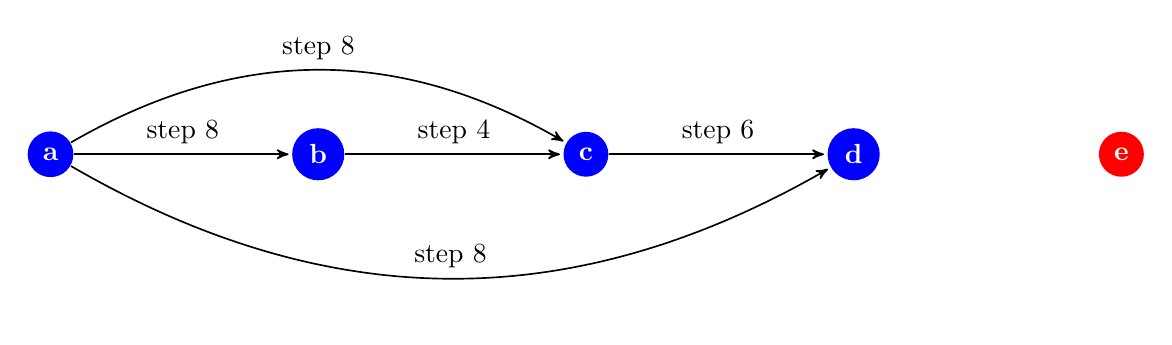
\begin{tikzpicture}[->,>=stealth',shorten >=1pt,auto,node distance=3.4cm,semithick]
  \node[shape=circle,fill=blue,text=white,draw=none]         (A)              {$\zdev{a}$};
  \node[shape=circle,fill=blue,text=white,draw=none]         (B) [right of=A] {$\zdev{b}$};
  \node[shape=circle,fill=blue,text=white,draw=none]         (C) [right of=B] {$\zdev{c}$};
  \node[shape=circle,fill=blue,text=white,draw=none]         (D) [right of=C] {$\zdev{d}$};
  \node[shape=circle,fill=red,text=white,draw=none]          (E) [right of=D] {$\zdev{e}$};

  \path (A) edge                node {step 8} (B) edge [bend left]    node {step 8} (C) edge [bend
            right]   node {step 8} (D) (B) edge                node {step 4} (C) (C) edge
            node {step 6} (D);
\end{tikzpicture}
\caption{Device approval graph, where nodes are devices and edges are approvals.}
\label{fig:devices}
\end{figure}

\subsubsection{Per-User Keys}
\label{subsubsec:puks}

One application of the trust graph is to facilitate \textit{per-user keys} (PUKs): a set of keys
shared between all of a user's devices, rotated on device addition or revocation.

In each $\deviceadd{}$ or $\devicerevoke{}$ operation, devices generate a new PUK seed. The PUK seed
is encrypted for each unrevoked device's device key: devices implicitly trust all older devices
(otherwise, they would revoke them). Each seed is associated with a number called a \textit{PUK
generation}, which starts at 1 and increments every time the seed rotates. All devices within an
approval class share the same set of known PUK seeds.

From each PUK seed, devices generate subseeds, symmetric subkeys, and asymmetric subkeys for various
applications such as email and voicemail.

Symmetric PUKs facilitate syncing encrypted data between a user's devices. Devices use the latest
per-user key to encrypt all content, but previous per-user keys are still useful for decrypting
older data. In the above example, if $\zdev{f}$ is provisioned, it doesn't yet have access to older
PUKs; only the one it just created. But if an older device performs a $\batchapprove{}$ that
includes $\zdev{f}$, it will also encrypt all the PUK seeds it knows about for the devices it's
approving, which means $\zdev{f}$ can now decrypt data encrypted with keys created before $\zdev{f}$
was introduced.

Asymmetric encryption PUKs can be used to encrypt data for other users. In particular, since version
6.3.0 of the Zoom client, we use both X25519 and Kyber768 keys to provide post-quantum secure
hybrid encryption, as detailed in Section~\ref{subsubsec:sigchainpqsecurity}. If Alice encrypts a
piece of content for Bob using his most recent asymmetric PUK, Bob can read the content on all
devices added before the content was encrypted, as well as all the devices added afterwards, as long
as those devices have been approved by an earlier one. The public keys corresponding to the
asymmetric keys derived from the PUK seed are published in the user's sigchain
(Section~\ref{subsubsec:usersigchains}).

To generate a set of PUKs, devices use the following key derivation. Each invocation of HKDF
uses a distinct context string.

\begin{enumerate}
\item
Generate a new 32-byte secret seed
\item
Use HKDF on the seed to generate different 32-byte keys:
\begin{enumerate}
    \item X25519 keypair
    \item Kyber768 keypair
    \item email seed (using HKDF to derive the following 32-byte keys)
    \begin{enumerate}
        \item X25519 keypair for email
        \item Kyber768 keypair for email
    \end{enumerate}
    \item voicemail seed (using HKDF to derive the following 32-byte keys)
    \begin{enumerate}
        \item X25519 keypair for voicemail
        \item Kyber768 keypair for voicemail
    \end{enumerate}
    \item symmetric
\end{enumerate}
\end{enumerate}


See Appendix~\ref{appendix:multidev} for a deeper analysis of multi-device configurations and the
guarantees we can achieve given these rules. In summary, a newly-added device will immediately be
able to send and receive new encrypted content that is accessible from all devices. Approving a
device will give that device access to past encrypted content. If a device is revoked, that device
is unable to decrypt any content encrypted after the revocation.

Note that if a device is self-revoked, the necessary key rotation might not happen immediately if
there are no other suitable devices online to perform it. Before the key rotation is completed, we
rely on the server to enforce that the revoked device does not access further user data, including
ciphertexts sent both before and after the revocation, by no longer accepting the per-device
authentication tokens and signatures using the keys the device owns. This is not a cryptographic
guarantee and relies on the server's honesty, and also does not cover any content already in the
device's memory before revocation.

\subsubsection{Backup Keys}
\label{subsubsec:backupkeys}

In addition to their physical devices, a user can add so-called ``virtual devices'' to their
sigchain. Virtual devices also have signing and encryption key pairs associated with them, but
instead of strictly corresponding to the physical device that generated them, these keys may be
exported or communicated to other parties and are used to provide additional functionality. Virtual
devices are treated like physical ones: they can be added and removed from the user's device list,
other devices encrypt PUKs for them, and the corresponding private keys can be used to approve other
devices or rotate PUKs.  

A backup key is a string of letters and digits which the user can write down on paper. By entering
the string on a new device, the user can decrypt and recover their encrypted data if all other
existing physical devices become unavailable.

Backup keys can be generated by one of the user's existing devices. Note that the backup key can
have at most the PUK access of the generating device. Backup keys are added to a user's device list
using a $\deviceaddandapprove{}$ operation (which combines $\deviceadd{}$ and $\batchapprove{}$, as
described above).

The device generates a high entropy string, which is displayed as a sequence of letters and digits,
such as
%
\[ \texttt{ZR30 4D11 5HJM RJG2 6H75 78DH B0VS 4KSF}. \] 
%
The first four characters are used as a key identifier and are not considered private. Backup keys
have at least 128 bits of private entropy, as well as built-in error correction to tolerate small
copy-pasting mistakes. The backup key string is used to derive a seed using
sodium{}'s~\cite{libsodium} \texttt{argon2id}, which is then used to derive the device's signing and
encryption keys.

Assume a user provisions a new device and does not have access to any of their previous physical
devices (either temporarily or permanently). The user can enter a backup key on this new device to
recover all the data available to the backup key: the new device will use the backup key to
re-derive the signing and encryption key corresponding to the virtual backup device and then perform
a $\batchapprove{}$ operation. In particular, the backup encryption key can be used to encrypt all
the PUKs that the backup device had access to for the current device's key.

\subsubsection{Escrow Keys}
\label{subsubsec:escrowkeys}
\emph{Escrow} (see Section~\ref{subsec:keyescrow}) allows accounts to designate some of their
members as \emph{Escrow Administrators (EAs)}, who can access other account members'
(\emph{escrowees'}) encrypted data in order to support features like legal discovery, retention, and
accidental loss prevention\footnote{Some companies are required by law to keep records of all their
communications, and make them available to law enforcement when requested. In addition, employees'
devices might get lost, stolen or otherwise unavailable.}. To support these use cases, an account
can enable escrow, which prompts each account member with an unskippable notification to add a
virtual device to their device list, the \emph{escrow device}, whose secret keys are encrypted for
the EAs.

The escrowee (or potentially one of their account's EAs) can rotate their escrow device's key (and
therefore concurrently rotate their PUK) whenever one of the EAs' devices with access to the
escrowee's keys is revoked (see Section~\ref{subsubsec:escrowmgmt}).

\subsubsection{Lockdown Mode}
\label{subsubsec:lockdownmode}
\textbf{Note:} As of version 5.15.10, lockdown mode is only available (and required) for EAs (see
Section~\ref{subsubsec:escrowadmins}).

As detailed in Section~\ref{subsec:multidev}, a standard user can add new devices at any time, and
start using them immediately (except for accessing previously encrypted data) without approval from
previous devices. This allows newly added unapproved devices to immediately start using E2EE Zoom
products to send encrypted data on behalf of the user, while not granting it access to previously
encrypted data until a previous device comes online to approve it. While this device model may be
appropriate for most users, some users may benefit from additional security guarantees, namely that
new devices cannot be used without the consent of an existing device. This prevents a compromised
server or an attacker who learns the user's password from adding a device and impersonating the user
without prior user approval%
%
\footnote{ Note that compromising the server would allow an attacker to temporarily reassign a
user's email identifier to a user whose keys are controlled by the attacker, thus circumventing the
need for prior approval for impersonation even if lockdown mode is enabled. This attack would still
be detectable after the fact, and currently is not applicable: only EA sigchains can enable lockdown
mode, and they do not have email identifiers.}%
%
(though imposing additional usability burden on the user).

Lockdown mode can be enabled or disabled for the user from a user's device in the oldest non-empty
approval class. When in lockdown mode, new devices can be added, but are not permitted to rotate the
PUK or approve new devices on behalf of the user until they are themselves approved by a device in
the oldest class (and thus join that class). We refer to these new devices as \textit{unconfirmed},
and older devices in the oldest class as \textit{confirmed}.

If a confirmed device revokes an unconfirmed device, no key rotations are needed (as the revoked
device did not have access to any PUKs). If a confirmed device approves an unconfirmed device, the
existing PUK is encrypted for the newly confirmed device, again without rotations. The PUK is only
rotated if a confirmed device revokes another confirmed device, including itself (although in the
self-revoke case, the rotation will be performed by another confirmed device once it comes online).
Unconfirmed devices are allowed to perform revocations of any device, but other clients will not
accept any PUK rotations performed by unconfirmed devices while the user is in lockdown mode.

Lockdown mode reduces the number of necessary key rotations, in addition to preventing a compromised
server from impersonating a user. On the other hand, the user will need to have access to at least
one confirmed device in order to add and use new devices. If the user loses or revokes all of their
devices, then data encrypted for their user will unrecoverable, and their account will be
essentially unusable.

The ``locked out'' user would have to create a new user account (note that Zoom allows email
addresses to be re-assigned). To reduce the likelihood of this ``locked out'' scenario, the Zoom
server requires users to create a backup key (see Section~\ref{subsubsec:backupkeys}) before
entering lockdown mode. The server enforces that users in lockdown mode have at least one unrevoked
device. One exception to this is that if an account disables escrow, the server will revoke all
devices belonging to the account's EA.

\subsection{Consistent Identities With Sigchains}
\label{subsec:sigchains}

Both accounts and users have states that change over time. An account can change its identity
provider or its ADN, and a user can change their email address or add and remove devices.

We need to keep track of states that change over time in a way that is auditable. To do so, we
describe the sequence of changes in a data structure called a signed hashchain, or
\textit{sigchain}.

Once a client learns of a sigchain, the only changes to this chain that will be considered valid are
extensions of the sequence. Since changes cannot be ``forgotten,'' the Zoom server cannot rewrite
history.

Still, this model doesn't force the Zoom server to be consistent across different devices it talks
to. We will add a transparency layer called the Zoom Transparency Tree (Section~\ref{sec:ztt}) to
ensure that the Zoom server must present the same information about sigchains to all users.

\subsubsection{Sigchains}

A sigchain is a sequence of statements (called \textit{links}), where each link includes a
collision-resistant hash of the previous link. These links can be thought of as state transitions
that modify an object (the sigchain state). For a user sigchain, the sigchain state contains the
list of active devices, the list of revoked devices, the trust graph, and the list of email
addresses and accounts historically associated with the user.

In order to accept a transition as valid, clients check that it satisfies several conditions,
including that:

\begin{enumerate}
\item The link is of a known type.
\item The link has the correct fields for that type.
\item The transition is admissible given the current state.
\item The link correctly includes the hash of the previous link.
\item Some links require cryptographic signatures by the devices authorizing the transition to be
    considered valid. In these cases, the signatures are encoded as part of the links to compute
    link hashes.
\end{enumerate}

Examples of admissibility rules for a user sigchain include that a device can only be revoked if it
was active in the previous state, and that signatures over revocation links must be by a device that
was active in the previous state.

Since each of the links in a sigchain contains a hash of the previous link, the hash of the last
link is a compact commitment to the entire sigchain state. Each sigchain link also contains an
incrementing sequence number. We refer to an object consisting of the sigchain type, the last link's
sequence number, and the last link's hash as the \textit{sigchain tail}:

\begin{Verbatim}
{
  "sigchainType": "User",
  "lastSequenceNumber": 15,
  "lastLinkHash": "484ad7..."
}
\end{Verbatim}

When clients want to update their view of a sigchain from the server, they can just query for the
new links and ensure that the first new link contains a previous hash matching the cached tail.

Note that the examples of objects in this document are encoded in JSON and simplified for ease of
exposition. The actual implementation may use different application encodings and data structures.

Different applications require different levels of access to sigchains. For example, although a user
should be able to fully audit the history of past email addresses stored in their sigchain, meeting
participants might only need to see the most recent one to display it in the UI\@. For this reason,
rather than being directly encoded, sensitive information on a sigchain link is stored as a
commitment: rather than \texttt{alice@example.com}, a sigchain link could contain
$$\mathsf{COMMIT}(\texttt{alice@example.com}) =
    \mathsf{HMAC}(\mathsf{randomKey}, \texttt{alice@example.com}).$$ %
The server gives all users the entire sigchain link so that they can check that its signatures
and hashes are valid, but only Alice's devices will receive the plaintext email addresses and
32-byte random keys corresponding to previous email addresses. \textsf{COMMIT} can also be used
to selectively delete parts of links such as device names: a server can throw away the random
HMAC key as well as the plaintext data, and the signature over the link will still verify.

\subsubsection{Overview of Sigchain Types}

Zoom devices, users, and accounts are each internally identified by unique immutable identifiers
called \deviceid, \userID, and \accountID respectively. The \deviceid is generated randomly for each
new device, while the \userID and \accountID are assigned by the server.

Each device, user, and account is also associated with more user-friendly (but mutable) identifiers:
respectively, device names, email addresses, and ADNs.

Representing these different components and their relationships requires different types of
sigchains:

\begin{enumerate}
\item User sigchains store, for each \userID, information related to that user's identity, such as
    the user's email address, \accountID, and the set of their devices and their trust
    relationships.
\item Email sigchains store, for each email address, the associated \userID.
\item Account sigchains store, for each \accountID, both the ADN and identity provider associated with
    the account.
\item ADN sigchains keep track of, for each domain name, the \accountID to which the domain is
    associated.
\item Membership sigchains keep track of, for each \accountID, the {\userID}s within the account.
\end{enumerate}

Note that some of the information stored on these sigchains is redundant: for example, a mapping
between an email and the corresponding \userID is recorded both in a user sigchain and in an email
sigchain. This is necessary so that the server cannot claim that two separate {\userID}s are
associated with the same email address at the same time. Accordingly, some operations will cause
multiple chains to be updated at the same time.

As detailed earlier, every Zoom user is part of an account. As potential optimizations, if this
account only has a single user and doesn't have an ADN, then that user's sigchain might not mention
their \accountID, and there would be no corresponding account or membership sigchains until the
account either gets another user or an ADN.

\subsubsection{User Sigchains}
 \label{subsubsec:usersigchains}
User sigchains record changes to a user's identity. There are several types of user sigchain links,
each representing a different way to change a user's identity.

\paragraph{EmailChange.} As mentioned in Section~\ref{subsec:displayid}, users can set and change the
email addresses that will be displayed for or used to communicate with other users. Two users can switch email addresses,
but the server will prove that two users do not have the same email address at the same time. An
\textsf{EmailChange} link will have the following fields:


\begin{Verbatim}
{
  "sigchainType": "User",
  "linkType": "EmailChange",
  "sequenceNumber": 10,
  "prev": "484ad7...",
  "cloudName": "commercial",

  "userID": "ebc0d2...",

  "emailChange": COMMIT({
    "email": "alice@example.com",
    "emailChainSequenceNumber": 5
  })
}
\end{Verbatim}

The first six fields are common to every sigchain link. \textsf{sequenceNumber} is an incrementing
counter that starts from 1 for the first link, \textsf{prev} is the (canonical) hash of the previous
link in the chain (in this case, the one with sequence number 9), and \textsf{cloudName} specifies
which cloud the sigchain belongs to.

Every user sigchain link also specifies the \userID.

Here, the \textsf{email} field specifies the new email address to be associated with this user,
which supersedes any previous email. Every time an \textsf{EmailChange} link associates this user
with a new email, the email sigchain for that email address is also extended with a corresponding
\textsf{UserIDChange} link referring to this user's \userID, and the sequence number of that link is
reported in this link as \textsf{emailChainSequenceNumber}.

Because the Zoom website can be used to change one's email address, \textsf{EmailChange} links do
not have any signatures (i.e., they can be inserted into sigchains by the Zoom server).

\paragraph{AccountChange.} Users can also transfer between accounts, similarly to how they can
switch emails.

\begin{Verbatim}
{
  "sigchainType": "User",
  "linkType": "AccountChange",
  ...
  "accountChange": COMMIT({
    "accountID": "c2d8aa...",
    "membershipChainSequenceNumber": 12,
    "additionIndex": 5
  })
}
\end{Verbatim}

Since multiple users can be added to a membership sigchain in a single link, \textsf{additionIndex}
specifies the corresponding position in that link. If a user is removed from an account, the
\textsf{accountChange} section specifies \accountID \texttt{null} and the other two fields are
omitted.

Since Zoom servers are allowed to move users between accounts, \textsf{AccountChange} links do not
have any signatures.

\paragraph{DeviceAdd.} A device addition link specifies the long-term public device keys for the new
device and a human-readable name:

\begin{Verbatim}
{
  "sigchainType": "User",
  "linkType": "DeviceAdd",
  ...
  "deviceID": "ebc0d2...",
  "deviceName": COMMIT({
    "name": "Alice's Work Smartphone",
    "version": 1
   }),
  "deviceType": "PHONE",
  "deviceEd25519PublicKey": "ce8564...",
  "deviceX25519PublicKey": "ad7913...",

  "userEmailX25519PublicKey": "f40b66...",
  "userVoicemailX25519PublicKey": "d600fc...",
  "userX25519PublicKey": "c2cce1...",

  "revokeDeviceIDs": [
     "ac98ad...",
     ...
  ]
}
\end{Verbatim}

This link specifies a device identifier (unique among the devices associated with this user), a
signing public key, an encryption public key, as well as a device name and type. Note that the
device name is hidden by a commitment, because users other than the owner of the chain do not need
to see it. In order to support reusing names, the device name includes an incrementing version
component, which will be visible in the user interface. Device names allow the user to have a
human-readable, unambiguous way to distinguish their devices.

The link also specifies the new per-user key public keys. The encryptions of the new PUK seeds for
older devices are not represented within the sigchain link, but are sent separately to the server,
which propagates them to the older devices.

After the user adds a new device, they can immediately use it to revoke any existing undesired
devices, which justifies our claim that later devices should trust the validity of earlier
(unrevoked) ones.

To ensure that users know the corresponding device private key, each $\deviceadd{}$ link requires a
signature by \textsf{deviceEd25519PublicKey}.

\paragraph{UserRoot.} This link should always be the first link in a user's sigchain, and can only
appear as such. It is equivalent to a DeviceAdd and specifies all the same kinds of information
about the user's first device, but can also include \textsf{emailChange} and \textsf{accountChange}
fields, which convey similar information as the corresponding sigchain links. Including these fields
here allows us to reduce the overall number of sigchain links.

\paragraph{DeviceRename.} Users can change their device names if desired. This change is signed with
the device's public key.

\paragraph{DeviceRevoke.} When a device is stolen, lost, or no longer used for Zoom, the user should
revoke it. If one of the user's valid devices performs the revocation, it will also rotate the PUKs
and sign this link to guarantee integrity of the new key. If instead the revocation is done through
the Zoom website, the PUK cannot be rotated and no signature is made. After a device signing key is
revoked, it can no longer be used to sign sigchain links.

\paragraph{DeviceKeyRotate.} If a user suspects their device was temporarily compromised, or if they
have institutional key rotation policies, they might want to rotate their device keys and PUKs. This
operation keeps the same \deviceid but chooses new signing and encryption keys, as well as a new set
of PUKs, and uploads encryptions of each PUK secret known to the device for the new encryption key
so that the old encryption key can be safely discarded. This link is signed by the device's previous
public key in addition to the new key. As with $\devicerevoke{}$ links, the old signing device key
cannot sign further sigchain links.

\paragraph{BatchApprove.} A $\batchapprove{}$ link lets a device indicate that it trusts the
validity of all devices created after that device until the point in the sigchain where the
$\batchapprove{}$ link appears. To reduce the number of sigchain links, the user can also specify a
list of devices to revoke within this link. The link can specify a new set of PUKs, and this is
required if any devices are being revoked. This link is signed by the approving device, and can be
used to construct a trust graph as described in Section~\ref{subsec:multidev}.

\paragraph{DeviceAddAndApprove.} This link is equivalent to a fused $\deviceadd{}$ and
$\batchapprove{}$, but allows us to reduce the overall number of sigchain links and also guarantee
that intermediate states of some operations can't appear on the sigchain. It is posted by an
existing device, the approver, but also specifies a device identifier, name, and keys for a new
device. Uniqueness of the new device's identifier, name, and keys are enforced just like in
$\deviceadd{}$. This link implies that the approver trusts all devices created up to and including
the device being added by this link. Signatures from both the approver and the new device are
required.

\paragraph{PerUserKeyRotate.} If a device notices that a device revocation (either a self
revocation, or one from the website) has occurred after the most recent PUK was generated, the device
will perform another PUK rotation using a $\peruserkeyrotate{}$ link. This guarantees that even if
the revoked device was compromised, this newest PUK is still confidential. For personal storage,
staleness is not an issue, as any device trying to encrypt data will first rotate the per-user keys.
But if other users are encrypting data for a compromised PUK and the server cooperates, data could
be readable by a revoked device. This link is signed by the device that is rotating the PUK.

\subsubsection{Email Sigchains}

Users can change their email over time. It is important that at any specific point in time, each
email corresponds to a unique user, so that Zoom users can be unequivocally identified. Also, users
should be able to audit whether at any point their email has been associated with another user. We
record the mapping between an email and the corresponding {\userID}s in an email sigchain. These
sigchains only have one kind of link, \textsf{UserIDChange}.

\begin{Verbatim}
{
  "sigchainType": "Email",
  "linkType": "UserIDChange",
  ...
  "email": COMMIT("alice@example.com"),

  "userIDChange": COMMIT({
    "userID": "ebc03d...",
    "userChainSequenceNumber": 9
   })
}
\end{Verbatim}

The \textsf{userChainSequenceNumber} refers to the position in the user sigchain of the
corresponding \textsf{EmailChange} link (or the initial \textsf{UserRoot} link).

Since users can change their email on the Zoom website, this link does not require any signatures.

\subsubsection{Account Sigchains}

Account sigchains consists of two kinds of links, which record the identity provider and ADN that
each account is using. \textsf{IDPUpdate} links contain the domain name of the IDP (say
\texttt{examplecorp.generic-idp.com}). IDPs should not use the same domain for multiple accounts
to prevent equivocation of their attestations.

\begin{Verbatim}
{
  "sigchainType": "Account",
  "linkType": "IDPUpdate",
  ...
  "accountID": "abef02...",

  "idpDomain": "examplecorp.generic-idp.com"
}
\end{Verbatim}

\textsf{ADNChange} links associate an ADN with the account. Only the latest \textsf{ADNChange} link
is considered valid, and each one corresponds to an \textsf{AccountIDChange} link in the appropriate
ADN sigchain. If an account is no longer using an ADN, the \textsf{adnChange} section specifies ADN
\texttt{null} and the other field is omitted.

\begin{Verbatim}
{
  "sigchainType": "Account",
  "linkType": "ADNChange",
  ...
  "accountID": "abef02...",

  "adnChange": COMMIT({
    "adn": "example.org",
    "adnChainSequenceNumber": 9
  })
}
\end{Verbatim}

Links in account sigchains do not require any signatures.

\subsubsection{ADN Sigchains}

ADN sigchains track which \accountID a specific Account Domain Name is associated with. There is
only one type of link, \textsf{AccountIDChange}, which corresponds to and points to an
\textsf{ADNChange} link in the account sigchain for the appropriate \accountID:

\begin{Verbatim}
{
  "sigchainType": "ADN",
  "linkType": "AccountIDChange",
  ...
  "adn": "example.org",

  "accountIDChange": COMMIT({
    "accountID": "873c34...",
    "accountChainSequenceNumber": 29
  })
}
\end{Verbatim}

Links in ADN sigchains do not require any signatures.

\subsubsection{Membership Sigchains}

Membership sigchains record changes to the set of users which are part of each account. They have a
single type of link, \textsf{ChangeMembers}:

\begin{Verbatim}
{
  "sigchainType": "Membership",
  "linkType": "ChangeMembers",
  ...
  "accountID": "19aebb...",

  "added": [
    COMMIT({
      "userID": "db2f1c...",
      "userChainSequenceNumber": 9,
    }),
    ...
  ],
  "removed": [
    COMMIT({
      "userID": "9ae3d2...",
      "userChainSequenceNumber": 4
    }),
    ...
  ]
}
\end{Verbatim}

Each link can add or remove multiple users. Each user is hidden behind a commitment so that it is
possible to prove that an individual user is part of an account without also leaking the {\userID}s
of the other members that are being added as part of the same link. Hiding the {\userID}s of the
users being removed from the account would potentially make it harder to prove that a user is indeed
still a member of a specific account without opening all the commitments. We will solve this problem
in the future by leveraging the transparency layer, but until then, clients will not rely on these
sigchains, although the server will start keeping track of them.

Links in membership sigchains do not require any signatures.

\subsection{Sigchain Fingerprints}
\label{subsec:fingerprints}
A sigchain fingerprint summarizes a user's sigchains. It is constructed as a hash of the user's user
sigchain and account sigchain tails (note that this includes the user's present and past email
addresses, as well as the current ADN due to the reference in the account sigchain). Sigchain
fingerprints are useful in two contexts: to verify new devices before approving, and to verify the
keys used to communicate with other users.

During the device addition and approval process, a malicious insider has the opportunity to conduct
a MitM attack. After the new device is added, the insider creates a copy of the
user's sigchain but replaces the keys in the final $\deviceadd{}$ link with keys controlled by the
attacker, using the same device name. The forged copy is served to older devices while the honest
sigchain is served to the new device. When the older device sees the approval interface, only the
device name is shown, and so the user may be tricked into accepting the server's device
unintentionally (which would imply sharing all previously encrypted data with the attacker).
However, in this case the two devices would necessarily display different fingerprints (as they bind
to sigchains containing different keys, and the hash is collision resistant). Users concerned about
MitM attacks can check, before approving new devices, that the fingerprint shown on
the approving device matches the one from the device(s) they intend to approve. This ensures that an
attacker cannot interfere with the process and gain access to historical encrypted data.

Sigchain fingerprints are also useful when communicating with other users. For example, when a user
emails another user for the first time, a malicious server could potentially swap out the intended
user's sigchain for an entirely fabricated sigchain with devices controlled by the server. In these
contexts, the user interface will allow users to verify the other user's sigchain fingerprint before
sending the encrypted message. This process requires the two users to securely communicate
out-of-band (for example, in-person). The sender can check that the fingerprint they see in their
client matches the recipient's fingerprint to ensure the message can be decrypted only by the
intended recipient. Similarly, the recipient can do the same for the sender to verify that the
message came from the expected sender and was not altered.

In the user interface, fingerprints are represented in hexadecimal. Users can always view their own
fingerprint from the Zoom client, and Zoom products will show the fingerprints of other users in
specific scenarios where it is useful.

\subsection{Backup Keys}
\label{subsec:backupkeys}

A backup key acts as a ``virtual device'' that can be added to a user's sigchain. Instead of
corresponding to an actual device, it is simply represented as a string of letters and digits, such
as
\[ \texttt{ZR30 4D11 5HJM RJG2 6H75 78DH B0VS 4KSF}. \] The first four characters are used as a key
identifier and are not considered private. Backup keys have at least 128 bits of private entropy, as
well as built-in error correction to tolerate small copy-pasting mistakes.

From a trusted device's Zoom client, a user can generate a backup key and add it as a new ``device''
to the user's sigchain with a $\deviceaddandapprove{}$ link. The backup key string is used to derive
a seed using sodium{}'s~\cite{libsodium} \texttt{argon2id}, which is then used to derive the
device's signing and encryption keys. Like normal devices, backup keys can be revoked.


\subsubsection{Account Recovery}

In the case that a user loses all their devices, they can log onto another device and enter their
backup key to write a $\batchapprove{}$ link to the user's sigchain that originates from the backup
key. This gives the new device access to all the old PUKs that the backup key had access to.

\subsubsection{Using Backup Keys for Escrow}\label{subsec:backupkeyescrow}

\textbf{Note:} Escrow using backup keys is not currently available. Users can still
manually generate backup keys and send them to their IT administrator out of band.

Organizations using Zoom may wish to have access to E2E communications involving their members, to
protect against data loss or to support legal retention and discovery. We refer to solutions that
give such organizations cryptographic access as \textit{escrow}.  While we are building a more
usable and robust escrow solution, backup keys can initially provide the minimal necessary
functionality: users can generate backup keys and send them to their IT department for safekeeping.
When escrow is enabled for an account, users in that account are notified before they are allowed to
continue use of Zoom products. Each user receives notice that their data is being escrowed the
first time they access their Zoom Mail Service email on one of their devices. The user should verify
the escrow administrator's sigchain fingerprint before continuing, after which the user's client
automatically sends an end-to-end encrypted email with a backup key to their account administrator.


\subsection{Client Key Management}
\label{subsec:clientkeys}

\subsubsection{Storing Secret Keys on Device}
\label{subsec:lks}

Clients persist device key pairs indefinitely until a $\devicerevoke{}$ or $\devicekeyrotate{}$
occurs. Device keys are never transmitted to any other device or the server. They may sometimes be
lost after a disk corruption or operating system reinstall. In this case, the user must go through
the provisioning process once again as a new device would.

Long-term device keys are stored in the local operating system's keychain (where available), but
with some added protection for two Zoom users using the same OS account.
%
Before storing keys in the local OS-provided keychain, we encrypt them using a key-wrapping key
stored by the server and specific to each user and each device. 
%
When a user revokes their device, they will delete the keychain entry and the server will delete the
corresponding key. This also guarantees that keys cannot be recovered from a backup of a device that
has since been revoked.
%
If two users are using the same computer, the key-wrapping key prevents one user from being able to
access the other's keys. 

One exception are keys corresponding to devices on the EA sigchain (see
Section~\ref{subsubsec:escrowadmins}). These keys are also stored in the OS keychain, but they are
encrypted using a key-wrapping key which is unique to each EA sigchain and each device. The server
will only provide this key-wrapping key to users with EA permissions (see
Section~\ref{subsubsec:escrowadminperm}). This allows two EAs in the same account sharing the same
device to use the same EA device key, which therefore only needs to be provisioned (and approved)
once.

We use the committing AEAD scheme $\mathsf{CtE1}$~\cite{messagefranking} to prevent the server from
supplying malicious key-wrapping keys.
%
On provisioning, after generating the device encryption and signing key pairs, the client will
encrypt each secret key $k$ as follows:
\begingroup
\RaggedRight
\begin{enumerate*}
\item Generate a 32-byte random string $\mathsf{KWK}$ and request the server to store it
persistently associated with the user and device.
\item Define $\context \leftarrow \texttt{"Zoombase-1-ClientOnly-KDF-SecretStore"}$.
\item Compute $C \leftarrow \textsf{CtE1-Enc}(\textsf{K}{=}\textsf{KWK}, \textsf{H}{=}\context,
\textsf{M}{=}k)$, where $\textsf{H}$ is the associated data parameter for the underlying AEAD, and
store it in the system keychain.
\end{enumerate*}
\endgroup

For \textsf{CtE1}, we use \HMACSHATWO as the commitment function and
\sodium{}~\cite{libsodium}'s \linebreak \texttt{crypto\_aead\_chacha20poly1305\_ietf} as the AEAD.

We emphasize that this feature will not protect against an insider who also has access to a user's
device (for example, by colluding with another user using the same device). It will also not prevent
different users of the same device from installing malware to steal the other user's keys.

\subsubsection{Device Management Interface}
\label{subsubsec:devicemgmt}

We offer a dedicated UI to manage devices that are part of the user's sigchain, available in the
Zoom client's settings. Upon visiting this device list, clients ask the Zoom server for the latest
sigchain tail and process any new links in order to make sure that the view is up-to-date. The
device list contains all active devices (which can be used to participate in E2EE communications)
and revoked devices (which can no longer be used), indicating their device name and type based on
the sigchain;\footnote{The list may also include some information about devices that is not directly
stored on the sigchain and that we rely on the server to report honestly. For example, it may
include the earliest time of any E2E-encrypted communication decryptable by each device, determined
as the time at which the oldest device in its approval class was added.} it also has the user's own
fingerprint and the user's current and past email addresses (if any). Users can revoke devices from
this view. If a device realizes that it is revoked (by processing updates to its own sigchain, for
example as part of a periodic refresh or because of a server notification), it will delete all
private ephemeral and long-term keys as well as sensitive data, and then log itself out.

When the user first uses a feature that requires sigchains from one of their devices, that device
generates a new set of device keys and adds them to the first link in the user's sigchain. From then
on, the user's other devices (existing and future) will also generate their own keys and extend the
chain; each time, the user is prompted to review the device list and revoke any devices that are
unrecognized, lost, stolen, or no longer used.

In addition, after provisioning each new device, the user gets notifications on their old devices
asking them to approve or revoke any new untrusted devices. This list might include devices that are
already revoked but are still new from the perspective of the old device. Users also get
notifications regarding changes made to their email address.

Once the Zoom Transparency Tree (Section~\ref{sec:ztt}) is deployed, Zoom servers and insiders will
not have the ability to, e.g., suppress notifications in order to hide a malicious device addition
or email change.

\subsection{Account Escrow}
\label{subsec:keyescrow}

Some of the data that organizations store on the Zoom platform is encrypted with Device Managed Encryption, where the secret keys are only
known to the devices of the users authorized to access it; the data is not available to Zoom
servers. For example, some emails between active users of the Zoom Mail Service (Section~\ref{sec:email})
and some phone calls between Zoom Phone clients (Section~\ref{subsec:phone}) are
encrypted using the sender and recipient's keys only. However, administrators of these organizations
may also wish to have access to this data, for example, to protect against accidental data loss (if
the account member loses their devices) or to support legal retention and discovery. We refer to
solutions that give such organizations cryptographic access to their members' encrypted data as
\textit{escrow}, and in this section we present Zoom's solution to this problem.

When an account enables escrow, all the account members (\emph{escrowees}) receive an unskippable
notification informing them that escrow is being enabled. Upon acknowledgement, each member adds a
``virtual'' escrow device (Section\ref{subsubsec:escrowkeys}) to their own user sigchain. This
escrow device's public keys corresponds to secret keys known to a set of devices which are
controlled by \emph{Escrow Administrators (EAs)}, account members designated with escrow
permissions. This enables all account members to automatically share their PUKs (and by extension
their encrypted data) with these admins.

\subsubsection{Escrow Administrators and the EA Sigchain}
\label{subsubsec:escrowadmins}

To enable escrow for their account, an account administrator assigns EA permissions
(Section~\ref{subsubsec:escrowadminperm}) to one or more users to designate them as EAs. EAs will
then be able to provision one or more of their devices with fresh \emph{EA device keys}, which
ultimately will be used to decrypt the encrypted content escrowed from all the account's users.

EA device keys are independent of the device keys listed on the EA's own user sigchain (and used to
encrypt their own data); instead, the EA enabled devices and their public keys are added to a
special user sigchain, which we call the \emph{EA sigchain}. EA sigchains follow all the rules of
regular user sigchains (Section~\ref{subsubsec:usersigchains}), but they have no associated email,
and devices listed in this chain can belong to different EAs (instead of a single user).

In addition, the server adds an \textsf{EscrowAdmin} link to the account sigchain referring to the
EA sigchain's $\userID$, so that account members can be on the same page on whether escrow is
enabled or not. Each EA sigchain is associated with at most one account, and vice versa.

When provisioning an EA's device to have access to all the account's data, the device generates
fresh EA device keys and adds a new link to the EA sigchain. These users' devices therefore have two
sets of device keys: one on the user's own sigchain, and one on the EA sigchain. Once it is approved
by an existing device on the EA sigchain, the device will receive all the PUKs associated with this
EA sigchain, allowing it access to all the escrowed data. Provisioned EA devices will display to
their corresponding EA users the list of active EA devices (which EAs can use to monitor which
devices have access to the account's data) and the EA sigchain fingerprint. Monitoring EA devices
and comparing fingerprints prevents MitM attacks. The fingerprint can be compared before approving a
new EA device, and shared with all the account members so that they can confirm it before enabling
escrow. After enabling escrow, account members can continue to monitor the EA fingerprint to ensure
that their escrow devices are rotated for every EA PUK rotation.

Given that the Zoom server is responsible for enforcing which users are EAs, and therefore can add
devices to the EA sigchain, the first device will enable lockdown mode on the EA sigchain (see
Section~\ref{subsubsec:lockdownmode}), and members' clients will enforce that this is the case. This
prevents an attacker compromising the Zoom server from generating new PUKs on the EA sigchain and
therefore gaining access to account members' data. Lockdown mode also avoids having to rotate the
PUK whenever a new device is added to the EA sigchain, which has a significant performance impact as
it would trigger a PUK rotation in all the account member's chains as well
(Section~\ref{subsubsec:puks}).

When an account administrator disables escrow, the Zoom server revokes all escrow admin management
permissions, adds a new link to the account sigchain with an empty escrow admin {\userID}, and
revokes all device keys on the EA's chain. As soon as clients are aware of this, either through a
server notification or from their own monitoring, they revoke the virtual escrow devices from their
own chains (and rotate their PUKs). EAs' devices will also revoke the EA device's secret keys from
durable storage. If the user is moved between different accounts, and the new account has escrow
enabled, the user will be notified of the new escrow being setup and given the opportunity to check
the new EA sigchain's fingerprint. If the former account has escrow enabled, those EAs will only
have access to the user's ciphertexts before the account change, while the user's devices will share
all known PUKs with the new EAs. As detailed in the Security Limitations section, we rely on the
server to enforce proper access control for cyphertexts when the encryption keys cannot be promptly
rotated due to the user's devices being offline, which can happen in both the above cases.

It is important that the EAs maintain access to at least one device in the oldest non-empty approval
class at all times, as otherwise escrowed data could be irreparably lost. For this reason,
administrators are required to generate a backup key on the EA sigchain when enabling escrow. If all
the devices on the EA's oldest class are unavailable, the only option to recover is to turn escrow
off and back on, which would trigger notifications to all account members to acknowledge escrow
again.

When escrow is enabled, or re-enabled when old escrow devices are unavailable, the new EAs will have
access to a specific user's data only after that user comes online to encrypt their keys for the
EAs. Therefore, there may be unrecoverable gaps in the content that can be recovered for the
escrowed users. To avoid this, we recommend account administrators to enable escrow before
encryption features that depend on the key management infrastructure we describe (such as Zoom Mail
Service and Restricted Voicemails), to avoid turning escrow off and on, and to generate
multiple EA backup keys and keep them in safe locations.

\subsubsection{Users' Escrow Device Management}
\label{subsubsec:escrowmgmt}

When an account enables escrow and sets up an EA sigchain, all devices belonging to the account's
members will receive an unskippable notification that escrow is being enabled for their account, and
that the user's data will be available to the account's EAs. Clients will validate that escrow is
turned on by checking that the EA sigchain's \userID{} is in the account sigchain, and only accept
EA sigchains with lockdown mode enabled.

The notification shows the EA sigchain's fingerprint, which account admins should share with their
users through a secure out-of-band channel. Users should compare the fingerprint received from the
out-of-band channel with the one displayed by their clients. If the fingerprints differ, users
should reach out to their account admins to notify them of the potential MitM attack. Users will not
be able to use features leveraging their device keys until escrow is enabled.

Upon acknowledgement of the notification, clients generate a fresh set of device keypairs
corresponding to their new virtual escrow device, encrypt the secret keys for the EA sigchain's
latest PUK, delete the secret keys, and add the corresponding public keys with a
$\deviceaddandapprove{}$ link on their own sigchain. The server will prevent users from revoking
this virtual device (unless the administrators disable escrow).

If the EA sigchain's PUK rotates, the escrow device keys of all the users in the account (and their
PUKs) have to rotate as well, as all those keys are known to a revoked device. A
$\devicekeyrotate{}$ link that rotates an escrow device’s key can either be signed by any of the
users’ own devices or by one of the EA's device keys. At the moment, these rotations are performed
by each user’s own devices when they come online, but in the future we can have the EA’s devices
also perform them to ensure that the escrow device key rotation is completed in a timely manner,
especially for users who might not come online frequently. Escrowee clients do not display UI
notifications for these escrow device key rotations, because the system enforces that the only
devices that can rotate the escrow device keys are those on the user sigchain, and those trusted by
the device on the EA sigchain that enabled escrow (and that the user has acknowledged they trust).
This is achieved by having clients enforce that the EA sigchain is in lockdown mode, and including
the EA sigchain tail in the $\deviceaddandapprove{}$ introducing the escrow device. If later the
client detects that the EA sigchain is no longer in lockdown mode, or that the device which posted
the latest PUK on this chain is not trusted by the one which originally enabled lockdown mode (for
example, this could happen when lockdown mode is disabled and re-enabled by a different device on
that chain), it either throws an error or asks the user to acknowledge escrow again (with an updated
fingerprint).

The Zoom server immediately notifies escrowee clients to handle escrow admin's PUK rotations; in the
future, users will monitor the Zoom Transparency Tree for the EA and account sigchains, which would
prevent the server from withholding such updates. When learning that the EA or account sigchain have
been updated, for example before performing an escrow device key rotation as above, clients enforce
that escrow is still enabled and that the \userID{} of the EA sigchain mentioned has not changed (by
looking at the account sigchain), and that the EA sigchain has lockdown mode enabled. If clients
detect that escrow has been turned off, or that the EA \userID{} has changed, they will revoke their
escrow devices from their own chains, rotate their PUKs, and potentially notify the user and
re-enable escrow as above using the new \userID{}.

\subsubsection{EA Permissions}
\label{subsubsec:escrowadminperm}
While all the EAs' devices in the oldest class have access to the same PUK keys and can perform the
same actions from a cryptographic perspective, the Zoom servers allow assigning a more granular set
of permissions to each Escrow Administrator, which would apply to all their devices on the EA
sigchain. These additional restrictions align with typical business requirements our customers might
have, as detailed below, but could be circumvented if the Zoom server were to be compromised.

Users with the \texttt{escrow-manager} permission can enable escrow, create the first escrow device,
grant escrow permissions to other users, and approve new devices on the EA sigchain.

To support user recovery (see Section~\ref{subsubsec:userrecovery}) and legal discovery (see
Section~\ref{subsubsec:legaldiscovery}), we introduce two more server-enforced permissions. 

Users with the \texttt{escrow-write} permission (used for recovery) and the \texttt{escrow-read}
permission (used for discovery) both can add devices to the EA sigchain, but cannot approve the
device themselves (only users with the \texttt{escrow-manager} permission can approve new devices
for the EA). Therefore, to receive access to the EA PUKs, their newly added devices need to be
approved by a user with the \texttt{escrow-manager} permission. In addition, users with the
\texttt{escrow-write} permission can use their EA device keys to write approval links on other
account member's user sigchains (therefore helping them recover their data), while users with the
\texttt{escrow-read} permission can request from the server ciphertexts encrypted for any of the
account member in order to decrypt them.

\subsubsection{User Recovery}
\label{subsubsec:userrecovery}

In the case that a user in an account with escrow enabled loses access to their devices (including
any backup keys), they can ask one of their escrow account administrator for help recovering their
data on a newly logged-in device.

An EA with the \texttt{escrow-write} permission can use one of their authorized devices on the EA
sigchain to approve the user's new device and give them access to the necessary encryption keys. As
in a regular device approval (Section~\ref{subsubsec:devicemgmt}), the EA is first presented with an
approval review screen which includes all of the escrowee’s devices (and the escrowee's fingerprint,
which can be checked out-of-band with them). If the admin accepts, the admin's device signs a
$\batchapprove{}$ sigchain link on the escrowee's chain, and encrypts all of the user's previous
PUKs for the user's new device. The EA signs the approval link with both the virtual escrow device
key (from the user's sigchain) and the escrow admin's own device key (from the EA sigchain).

\subsubsection{Legal Discovery}
\label{subsubsec:legaldiscovery}

Some situations, such as legal discovery, will require the account admin to obtain data from its
account members.

If escrow is enabled, an EA with the \texttt{escrow-read} permission can request from the server
escrowees' data ciphertexts (such as emails encrypted with escrowee PUKs) and ciphertexts containing
the escrowee PUKs (encrypted for the virtual escrow device, the secret key of which is known to the
EA devices), and therefore decrypt the necessary data without cooperation from other account
members.

\subsection{Highlighting Untrusted Devices with Contact Sync}
\label{subsec:contactsync}

\textbf{Note:} Contact Sync is not currently available. We plan to release it in a future update.
The description here is specific to E2EE Meetings (Section~\ref{sec:meetings}), but similar
guarantees can be extended to other products. 

Even with a strong concept of identity, impersonation attacks are still possible in meetings. If
Bob's coworker, Alice, has the email \texttt{alice@company.org}, Bob might not realize if he joins a
meeting with an impersonator using \texttt{al1ce@company.org}, especially if the impersonator has
their video turned off. Or if a hacker stole Alice's username and password, they could provision a
new device and pretend to be Alice. We'd like to have a TOFU-style UI feature to let Bob know if
it's the first time he's seeing a device in a meeting---but we also don't want to bother Bob for his
first meeting with Alice on every new device that Alice makes, which could lead to alert fatigue.
Specifically, we want to provide warnings when Bob is in a meeting with a device that is not
approved by a device that Bob has seen before. We'd also like Bob to share his meeting history
between his devices securely so they all have the latest information.

Each device maintains, for every other user that it has been in a meeting with, a record containing
that user's user sigchain tail, the time of their first meeting together, and the total number of
E2EE meetings they were in together. These records are updated after each meeting as appropriate,
though they are only updated when either
\begin{enumerate}
\item The meeting has less than 25 participants and the device has been in the meeting with the
participant for over 10 minutes
\item The participant has been speaking for over 30 seconds
\end{enumerate}

In order for the meeting history to be shared across devices, clients periodically send encrypted
meeting records to the server. Records are individually encrypted with the latest PUK, signed with
the device key, and tagged with $t = \mathsf{HMAC}(k, \userID)$, where $k$ is a key derived from the
PUK. The server stores a mapping between $(\deviceid, t)$ and the encrypted record, which the
clients can update as necessary. When the client learns of a new PUK, records and tags are updated
to use the new PUK lazily.

The records are encrypted to minimize the privacy loss in case they are leaked (Zoom servers already
learn who is participating in which meeting). Because the tag is generated deterministically, these
records would reveal if two of Alice's devices had meetings with the same user (but not which user),
given that both devices used the same per-user key. However, we find this tradeoff acceptable as it
allows for a more efficient synchronization. Further, the server has the ability to rollback a
device's record at any time, but doing so could only cause additional warnings.

When joining a meeting, clients generate tags for each other participant using each known PUK and
request the server to send any corresponding records. Any record signed by a revoked device is not
considered. Given this data, we can provide warnings for each device in a meeting:
\begin{enumerate}
\item If the device has been seen before, or if the device is trusted by a device that has been seen
    before as indicated by the trust graph, display the number of meetings with this user in the
    last month.
\item Otherwise, if the device is untrusted but the user has been seen before, display ``This is the
    first time you are talking to this device of this person."
\item Otherwise, display ``This is the first time you are talking to this person."
\end{enumerate}

Note that devices may not have access to all the per-user keys used to encrypt records, which could
result in extraneous warnings. For example, imagine Alice provisions Zoom on her phone and has a
meeting with Bob. Then, Alice provisions Zoom on her laptop and has another meeting with Bob without
approving the laptop from the phone. In this case, Alice's laptop does not have the PUK used by
Alice's phone to encrypt the record, so there will be another warning for Bob in the second meeting.

Though Contact Sync warnings improve Zoom users' security, alert fatigue can make the warnings less
useful. If a user's contacts regularly fail to approve new devices with earlier ones, or if the
server does not properly sync records of prior communication, users can grow accustomed to the
warnings and possibly ignore them in the event of a real attack. Even without an attack, excessive
warnings make for a suboptimal and tiresome user experience.

\subsection{Compromise Prevention for Device Provisioning}\label{subsec:realtime} \textbf{Note: }
The features in this section are not currently available. We plan to release them in future updates.

With the ZTT (see Section~\ref{sec:ztt}), we have a mechanism for users to detect sigchain
corruptions after-the-fact. For instance, if an insider adds a new device onto Alice's sigchain to
impersonate her in a meeting while she is offline, Alice will detect the attack after she comes back
online, since the attacker had to commit the malicious change to Alice's sigchain to the ZTT.
Ideally, Alice could prevent unauthorized device additions from happening in the first place. Note
that users whose identities are vouched for by a trusted third-party IDP
(Section~\ref{sec:idpattestations}) already have good protections as long as their IDP is not
compromised. We want to offer a strong alternative to all users that does not rely on external
parties.

Recall that users currently login to Zoom via SSO, OAuth, or simple username and password. Their
devices' keys are authenticated by multiple signatures: a self signature, an optional approval
signature by an older device (Section~\ref{subsec:multidev}), a signature by Zoom (as part of the
inclusion in the ZTT, once it is deployed), and an optional attestation from the IDP.

Further validations of the device keys are possible. For example, users can sign new devices with
existing devices at the time they are first added (as opposed to in a later approval), potentially
through a QR-code-based flow similar to the one Keybase has now. One device shows a QR code of a
random session key, and the other scans the QR code; this establishes an end-to-end secure tunnel
between the two devices that a compromised server cannot interfere with. Over this tunnel, devices
can exchange public keys and cross-sign each other.

Alternatively, organizations can set up policies that require an IT administrator to sign off on
device additions. The new user device can display the hash of its public key in QR code form. The IT
administrator can scan it, signing the new device with their administrator's signing key.

Devices without the required signatures might be prevented from signing on behalf of the user or
rotating the user's PUKs, thus denying them access to any content encrypted for the user. They might
also trigger extra UI warnings to other participants when joining meetings, or even be excluded from
meetings marked ``high security.''


\subsection{Security Properties}
\label{sec:IdKmProps}

The identity and key management system described in this section is leveraged by multiple Zoom
products, and it provides some lower level security properties that these products build upon.

First, we note that the secret keys corresponding to any device public keys included in any sigchain
are known only to the device that generated them (unless an attacker has somehow gained access to
the device's memory or storage): secret keys never leave the device,\footnote{Except possibly when
the user voluntarily sends crash reports to Zoom. We try to minimize this risk, but cannot exclude
it.} and are only used to perform encryption and signing. A consequence is that
ciphertexts/signatures for/by each of the device keys can only be decrypted/created by the device
that generated these keys. Virtual device keys are an exception. For example, backup keys are shown
once to the user as text strings that can be written down, and therefore our guarantees depend on
these keys being kept securely by the user, and not being available to an attacker. A second
exception is escrow keys, where the escrow device secret key is possibly generated by one of the
user's own devices and encrypted for the account's escrow admin's PUK: this gives the EA's devices
the same access to the user's keys as the user's own devices.

Similarly, consider any valid user sigchain. The secret keys corresponding to any per-user public
key that appears in that sigchain are only known to any devices that were added but not revoked
before the per-user key was added to that sigchain, plus any devices that were added afterwards and
approved by one of those devices (as recorded in each device's own view of the user's sigchain). If
escrow is enabled or the user creates backup keys, some EA devices and those with access to the
backup keys might also learn these PUKs.

Also, note that the Zoom server cannot force any devices to forget identity updates like device
revocations: when receiving sigchains, devices only accept new sigchain links that extend the ones
they are already aware of.

\subsubsection{MitM Between a User's Devices}
These properties allow us to obtain strong guarantees about the confidentiality of the data that is
encrypted for a user's device keys and PUKs. For example, consider any ciphertext (such as an email
draft) encrypted for a given per-user key whose secret key is only known to a set of uncompromised
devices controlled by the corresponding user (and the users who have permissions to manage the
escrow admin virtual user, if escrow is enabled). In order to obtain the plaintext, an adversary
(even an insider) would have to either break the encryption scheme, compromise one of the user's (or
escrow admin's) current devices or backup keys, or trick the user into using one of their devices to
approve a maliciously-controlled device (so that the existing device encrypts the PUK secrets for
the malicious one). If escrow is enabled, an adversary could also compromise one of the escrow
admin's device keys, or a malicious insider could trick the escrow admin user into approving a
maliciously-controlled device.

A cautious user would only approve an additional device on their sigchain in a situation where they
expect such a request: for example, after they sign in on Zoom for the first time on a new device,
or in the case of enabling escrow, after they receive a trustworthy notice from their account
administrator that escrow is being enabled. An insider could take this as an opportunity to attempt
a MitM attack, by lying about the new device's public key to the old device. However, outsiders
cannot perform this attack: even if the attacker had access to the user's credentials, the attacker
would have to add an extra additional device and cannot prevent the legitimate one from appearing in
the approval modal. Comparing the sigchain fingerprints as known to the approving device and the new
device before confirming approval (and comparing the EA's fingerprint before adding or approving the
virtual escrow device) also prevents insiders from performing this attack. Because the sigchain is
an append-only data structure, comparing fingerprints after approval would still allow the user to
detect the attack, providing evidence of server compromise/misbehavior and allowing the user to
mitigate its effects.

In the future, the Zoom Transparency Tree will offer (assuming trusted auditors) an automated and
transparent way to ensure that devices have a consistent view of all sigchains and public keys such
that checking fingerprints before device approvals will no longer be critical.

\subsubsection{MitM Between Different Users}
Another class of attacks involves an MitM between the sender and recipient of an encrypted
communication. An insider might lie to the sender about the recipient's sigchain and PUKs or add a
malicious device to the recipient's sigchain, causing the sender to encrypt for a key controlled by
the attacker. These attacks can be prevented or detected by checking fingerprints, and can in many
cases be detected after-the-fact with minimal user burden by leveraging the ZTT.

Consider an adversary compromising one of the recipient's devices or backup keys, thus obtaining
their secrets. With access to the device, an attacker could obtain all the recipient's data, both
locally cached and stored by the server (at least until their session expires). If the user
discovers the compromise, they could revoke this device and rotate their keys, preventing further
data leakage. However, if the attacker also compromises (even at a later point) the Zoom server
infrastructure, they might attempt a more subtle attack: when a sender requests this recipient's
sigchain, the server could provide a legitimate but stale version of this chain, i.e., one that does
not include the device revocation and the subsequent rotation. This attack can be prevented by
comparing fingerprints. However, detecting this compromise using fingerprints after the fact is not
that straightforward: the sender and recipient would have to ensure that they agree on their views
of the recipient's sigchain at the time the \emph{message was encrypted and sent}, rather than at
the time of the fingerprint comparison. Assuming all clients have synchronized clocks, one way to
achieve this would be to have each sigchain link include a timestamp. Each client would remember the
last time they updated their view of any sigchain and refuse to accept new links for that sigchain
that have an earlier timestamp. In order to be tolerant to time misconfigurations, we currently do
not enforce these properties, but we are considering them for future updates.

Eventually, the ZTT might also ensure, under similar time synchronization assumptions, that
everyone's view of all sigchains is not only consistent, but also relatively up-to-date, i.e.\ that
any attempt to withhold updates beyond some reasonable tolerance bound is detected. This will ensure
that the server is not able to trick senders into encrypting for out-of-date keys unnoticed.

\subsubsection{Post-Quantum Secure Hybrid Encryption}
\label{subsubsec:sigchainpqsecurity}
We also aim to defend against an adversary who is recording encrypted data today, expecting to be
able to break classical encryption at a later time using a quantum computer. Our protocol protects
against this threat by using the Kyber post-quantum secure key encapsulation mechanism. We recognize
that Kyber is a novel cryptographic algorithm and has been subject to less real-world scrutiny
compared to classical cryptographic algorithms such as X25519. Thus, we use a hybrid approach,
hashing the results of both a X25519 key exchange and the Kyber key encapsulation to derive shared
symmetric encryption keys, so that even if Kyber turned out to be flawed, the security of the
overall protocol would not otherwise be affected (beyond losing the post-quantum security). We
stress that, as detailed in Section~\ref{sec:background_and_goals}, we do not currently defend
against existing quantum adversaries, as our signatures are not post-quantum secure. 

Clients use post-quantum secure hybrid encryption with device managed keys to exchange seeds and
keys between each other, and for data encryption in products leveraging device-managed encryption
such as Zoom Mail Service (Section~\ref{sec:zoommailservice}). The details of the key derivation and
encryption format vary slightly by application, but are analogous to those used in the Zoom Meetings
E2EE protocol (Section~\ref{subsubsec:meetingcrypto}).

Post-quantum encryption support for device managed keys was added in Zoom client version 6.3.0. When
upgrading, clients generate Kyber768 device encryption keys in addition to their X25519 device
encryption keys, posting a $\devicekeyrotate$ link on the user's sigchain. Users also need to
regenerate all of their backup keys, as pre-existing backup keys do not have Kyber keys associated
with them. The user interface will indicate which devices and backup keys need to be updated to
generate Kyber768 keys.

The last of the user's devices to get upgraded will generate a new set of post-quantum per-user
keys, and can send the corresponding secret keys to the other devices (using their post-quantum
device keys, so that a post-quantum secret is always itself encrypted using post-quantum secure
encryption). From then on, other users can leverage post-quantum secure hybrid encryption to
communicate with this user, for example to send end-to-end encrypted emails. If a user hasn't
completed the upgrade process yet, we fall back to only using X25519 to derive encryption keys (as
detailed in previous versions of this whitepaper).

The user interface will indicate which devices have not yet been upgraded to generate post-quantum
encryption keys.

Note that, if the account the user is part of has escrow enabled, the escrow virtual device on the
user chain (Section~\ref{subsec:keyescrow}) needs to be rotated too. Therefore, escrow admins have
to upgrade all of their devices (so that post-quantum per-user keys are available on the escrow
admin sigchain) before their users can leverage post-quantum hybrid encryption. 

\subsubsection{Integrity}
Ensuring that all devices have a consistent view of a user's sigchain and that no extraneous devices
have been added to it (by comparing fingerprints or relying on the ZTT and monitoring one's own
sigchain) also helps with integrity guarantees. Users can ensure communications haven't been
tampered with by checking that they are signed by devices belonging to the claimed author. However,
as above, in some cases the evidence of compromise might be less conclusive: if the sender signs a
message using a device's signing key, and later revokes that device (for example, because the device
was lost or compromised), the recipient has no way to tell if the message was signed before or after
the revocation/compromise. The user interface may communicate this potential risk to the recipient
so that they can confirm the integrity of any sensitive communications with the sender out-of-band,
or ask them to resend the message with an up-to-date key.

\subsubsection{Security Limitations}

While our concept of identity provides strong security guarantees, there are still attacks it won't
be able to prevent.

An attacker who is able to register a new device in the system on behalf of a non-consenting user,
whether by stealing the user's credentials or compelling the server, will be able to read data that
is E2E-encrypted to the targeted user after the compromise (but not before, as explained above), as
it will be able to add a new compromised PUK to the user's chain, which might be used by other users
to encrypt messages intended for the recipient before the recipient has had a chance to come online
to review and revoke the new device. This attack can be prevented if the sending user compares
fingerprints out-of-band with the potentially compromised recipient(s) before encrypting for the new
PUKs, or detected by comparing fingerprints (possibly implicitly through the ZTT) after the fact.

When one of a user's devices is revoked, the per-user public encryption keys for that user become
stale and should be rotated as soon as possible. When another of the user's devices comes back
online, they will pick new encryption key pairs, publish the public keys in a new sigchain link, and
encrypt the secret portions for all the user's devices that are still active. If one of the user's
devices is revoking another one, key rotation can happen immediately. However, in case of
self-revocation or revocation from the web or by an account administrator, if none of the other
user's devices are online, this rotation might be delayed. A delay can also happen if escrow is
disabled, or the user is moved between accounts (with different escrow administrators) while being
offline. Any data encrypted to this user during this period would be using an encryption key known
to a revoked device (or to old escrow administrators' devices), and we rely on the server to enforce
that these devices can no longer access user data. An attacker who both compromised a revoked (or
escrow administrator's) device \textit{and} had read access to the server might thus be able to
decrypt this data. Although the attack window seems limited and hard to exploit in practice, this is
a limitation of the current design. Similarly, when a key is revoked and rotated out, we do not
re-encrypt old ciphertexts for the new key, and rely on the server for access control to the
ciphertexts.

We stress that, while escrow enables necessary enterprise features such as account recovery and data
retention, EAs' devices have keys that allow them to decrypt all data in their account: as such,
this privilege should be restricted to a few security conscious users to minimize the potential for
compromise.

\subsubsection{Privacy Limitations}

From a privacy perspective, in addition to the identifiers displayed in the user interface, our
solution provides some limited extra information about a user to other users they interact with: the
sigchains reveal the history of the user's devices, including when they were added and revoked (but
not their names, which are protected behind a commitment), as well as which device was used to sign
any specific E2E-encrypted communication. Similarly, the number of times that a user changes their
email address or account is visible (but not the previous emails or account IDs). Moreover, since
the server might report the timestamps of sigchain statements (and, once deployed, the ZTT will also
necessarily reveal the same information), time correlations between different statements might be
exploited to infer, for example, that two users swapped their email addresses, or that two users are
in the same account. While this information is not displayed in the user interface, the client needs
this data to perform the sigchain validation and therefore a motivated attacker might extract such
information. We believe that this is acceptable; it is similar to the security code change warnings
in applications like Signal and WhatsApp.

Note that sigchains are not publicly available and are subject to server-side access control: they
are provided as needed to users. For example, if Bob is a Zoom Mail Service user and knows Alice's
email address, they can ask the server for the sigchain associated with that address in order to
encrypt an email. We currently rate limit requests for users' sigchains and other personal data as a
partial mitigation for this leakage.

In the future, we are considering a different mechanism that allows the server to offer
``randomized'' versions of a user's encryption keys, in a way that trades the opportunity to check a
user's fingerprints (while still being able to detect impersonation after the fact) for increased
privacy.

    \section{Transparency Tree}\label{sec:ztt}
    \textbf{Note:} The Zoom Transparency Tree is not currently available. We plan to release it in a
future update.

In this section, we describe a mechanism that expands the authentication guarantees from
Sections~\ref{sec:identitykeymanagement} and \ref{sec:idpattestations} to ensure that all Zoom users
have a consistent view of each others' devices and keys.

Imagine an insider, Mallory, who wants to eavesdrop on a meeting between honest users Alice and Bob,
who have never interacted on Zoom before and haven't checked the meeting leader security code. To
succeed in this attack, Mallory could instruct the Zoom server to lie to Alice about Bob's keys and
to Bob about Alice's keys, replacing them with keys she controls. If Bob's client is the only one to
see the fake key for Alice, and similarly Alice's is the only client who gets the fake key for Bob,
then such an attack would be hard to detect after the fact.

Some possible countermeasures for such attacks require trusted external entities or manual
validation steps (such as checking the security codes described in
Section~\ref{subsec:securitycode}) that potentially have to be performed out-of-band. Instead, we
will be able to detect equivocation by Zoom servers and identity providers while minimizing active
checking by the user.

To do so, we will ensure that Zoom servers provide the same mapping between user accounts and public
keys to all clients, sign such a mapping, and are held accountable for these signed statements. This
way, in order to compromise a single meeting, Zoom would have to lie not only to Alice about Bob's
keys (and vice versa), but also to every other Zoom user about those keys, including lying to Bob
about his own keys. Bob's client can thus easily review the list of his devices and discover any
suspicious activity. External auditors will routinely verify that the server's mapping is consistent
over time.

Thus, key fingerprint comparisons and other related warnings can be demoted in the user experience,
to be replaced with targeted security alerts (which we expect never to be triggered). Key security
becomes virtually invisible to the user.

\subsection{Zoom Transparency Tree}

The idea that there should be a single and consistent mapping between an identity and its public
keys has already been explored successfully to solve similar issues. Most notably, Certificate
Transparency~\cite{langley2013certificate} limits the damage that a compromised certificate
authority can do by signing fake TLS certificates. It does so by requiring that all signed X.509
certificates must be submitted to a publicly auditable log before being accepted by browsers.
Industry projects such as Key Transparency~\cite{keytransparency} and Keybase~\cite{keybase} (which
is now part of Zoom) and academic works such as SEEMless~\cite{chase2019seemless} and
CONIKS~\cite{melara2015coniks} have explored applying a similar approach to individual users'
identities for messaging applications, with Keybase being the only instance in production use today,
as far as we know. However, all the existing solutions in this space that we are aware of do not
currently match Zoom's security and privacy requirements while offering usability features like
multi-device support.

We build on prior work to design a new mechanism tailored to Zoom's use cases: the Zoom Transparency
Tree (ZTT). The ZTT is backed by a Merkle tree as used by Keybase, but with privacy-preserving
path-lookup features as in CONIKS. This data structure offers a key-value store interface where
key-value pairs, once inserted, cannot be removed or altered. The state of the structure can be
summarized by a small commitment, and lookup queries can be accompanied by a short proof that they
are consistent with the commitment. Whenever a client is given a signed sigchain statement (as
introduced in Section~\ref{subsec:sigchains}) about another user's identity or their keys, this
statement is accompanied by an inclusion proof in the ZTT.

\subsection{Integration Details}

\subsubsection{ZTT Auditing}\label{subsec:zttaudit}

The design of the ZTT requires auditing to verify the structure of the tree. Zoom will partner with
independent external auditors which (in a privacy-preserving way) ensure that the append-only
property of the ZTT is respected.

Clients query the auditors to ensure that their view of the ZTT's commitment has been audited and is
consistent with everyone else's. If the client can reach the auditor and detects a fork in the ZTT,
they can send the auditor the forked and signed commitments in addition to the warning, so that the
auditor can disclose the inconsistency. If Zoom clients cannot reach any of the auditor servers,
they will signal a degraded encryption level.

We will publish code so that interested parties can also audit the ZTT.

Additionally, organizations using Zoom will be able to review updates to the ZTT and track their
employees' device changes.

\subsubsection{Provisioning}

When provisioning a new device, the client ensures that the sigchain statement is included in the
ZTT by first sending it to the Zoom servers and then querying the ZTT to check that the sigchain
update has been included.

\subsubsection{Self-Audit and Refresh}

Periodically, the user's client should ask the server for an updated ZTT commitment, ensure that
this commitment is consistent with past data, possibly verify it with external auditors, and review
the user's sigchain for any new statements. If new keys are added to the sigchain, the client should
ask the user to review the changes. If the user notices an unexpected change, they may be prompted
to change their password or talk to their IT department.

\subsubsection{Validating User Identity}

Because we only trust keys stored within the ZTT, users can verify that each others' public keys are
included in the ZTT, before proceeding with using the keys.

\subsubsection{Contact List Updates}

The contact lists that users accumulate, described in Section~\ref{subsec:contactsync}, can also be
stored in the ZTT. The immutability guarantees that the ZTT provides means that Alice can note an
update to Bob's identity in the client installed on her phone, and Zoom is obliged to relay that
update to her desktop client.

\subsection{Security Properties}

Though the ZTT allows an equivocating server to be detected, we rely on the user to validate device
additions. Users might be offline or might be ignoring notifications and therefore compromises might
not be detected, or only detected after an attack.

The ZTT requires external auditors to provide security guarantees. If the auditors are not honest,
or have poor uptime, this can limit the ability to detect server misconduct. We can mitigate this
risk by relying on multiple auditors or implement partial auditing by clients.

    \section{Identity Provider Attestations}\label{sec:idpattestations}
    \textbf{Note:} As of version 5.13.10, we only support Identity Provider
attestations that are issued by Okta and are displayed in the context of E2EE meetings.
This feature is called ``Okta Authentication for End-to-End Encryption''.

Accounts that have an ADN and a compatible identity provider\footnote{Compatible
identity providers need to support a custom extension of the OpenID Connect
(OIDC) protocol which we describe below.} (IDP) are able to have the IDP vouch
for their users' identities in a way that other Zoom users can independently
verify. This mechanism restricts the ability, even for Zoom insiders, to
impersonate account members. Many organizations already trust an IDP for
authentication purposes, so this feature does not increase the attack surface or
require additional trust in the IDP.

In order for clients to be able to verify identity attestations by an external IDP, we need two
components:

\begin{enumerate}
\item A way for clients to determine the IDP associated with a Zoom account (that cannot be
    tampered with by the Zoom servers)
\item A mechanism for IDPs to issue---and for clients to verify---a signed attestation that binds
    a user's email address to the cryptographic key(s) they use to communicate (see Section~\ref{sec:identitykeymanagement})
\end{enumerate}

\subsection{Associating Accounts with Identity Providers}
\label{subsec:adnToIdp}
In order to associate an account to its IDP, the account's ADN hosts a DNS
TXT record, per cloud, pointing to the corresponding IDP domain. Specifying the
cloud identifier in the record supports ADNs configuring different IDPs for
different clouds. Note that since accounts are expected to change their IDP
rarely, clients can cache this mapping aggressively.

For example, if an account hosted on the Zoom commercial cloud is using 
\texttt{example.org} as their ADN and \texttt{generic-idp.com} as their IDP,
then the DNS entry for \texttt{example.org} should include a TXT record
with a value like:
\begin{center}
    \texttt{v=zoomadn us.zoom.idp.commercial=examplecorp.generic-idp.com}
\end{center}


As part of the process of validating IDP attestations (see
Section~\ref{subsec:validateattestation}), clients request the IDP domain value
from the Zoom server, and compare it with the value returned in the account's
DNS TXT record. In addition, once the ZTT is deployed, clients will also check
that this information matches what is in the ZTT for auditing purposes. If the
values do not match, then clients won't complete verification of or display any
identifiers for the account's users.

\subsection{IDP Attestations}

IDP attestations are generated and verified according to the OpenID Connect (OIDC) protocol.
OIDC is an extension of the widely used OAuth 2.0 authentication protocol, an industry standard that
many IDPs and Single Sign-On providers already support. OIDC provides a standardized format, the
ID token, to express claims about identities and their attributes. It also specifies how users can
request attestations for their own identity and verify ones obtained from other users.

We customize the protocol by:

\begin{enumerate}
\item Introducing an additional attribute \texttt{"zoom-identity-snapshot"} to the ID token in order
    to encode the state of a user's identity on Zoom. The IDP keeps track of the latest value of
    this attribute for every account user.
\item Specifying how this attribute can only be updated by the authorized user, and not by any other
    user or entity, including Zoom servers.
\item Specifying how this customized ID token for a specific user identity can be validated by other users.
\end{enumerate}

Our modified OIDC ID token (which we will also refer to as an \textit{IDP
attestation}) is a signed JSON Web Token (JWT) data structure which contains
claims about a user’s Zoom identity. The payload might
look like the following:

\begin{Verbatim}
{
  "iss": "https://examplecorp.generic-idp.com", // issuer

  "email": "alice@example.com",

  "zoom-identity-snapshot": "409788…",

  "exp": 1311281970 // expiration time
  "iat": 1311280970, // issue time

  [...]
}
\end{Verbatim}

The token contains an \texttt{issuer} field which identifies the OIDC issuer of the token (the IDP). In
order for Zoom clients to accept an identity claim, the \texttt{issuer} field must match
the IDP domain associated with the account.
\texttt{iat} and \texttt{exp} specify the validity of the token. The
\texttt{zoom-identity-snapshot} field encodes the state of a user’s identity,
such as the user's sigchain-backed identity; it is treated by the IDP as
an opaque string, and the IDP does not need to check its validity (the identity
snapshot is further described in Section~\ref{subsec:snapshots}).  

The fetched attestation may be shared with and validated by anyone, so it
doesn't include the \texttt{aud} field. Unlike standard OIDC ID tokens, which
are ``bearer tokens'' in that they can be presented by a user to prove their
identity to the party indicated in the token's \texttt{aud} field, our
attestations are meant to be exchanged with potentially many other clients to
prove a binding of a particular client's identity to their keys. Because
compliant OIDC implementations enforce that the \texttt{aud} field contains
their own identifier, they will not accept our attestations (which lack this
field) as a standard ID token for authentication purposes.

The \texttt{email} value must match the email address that the user logged into
Zoom with (and that the server gives to the verifying client) in order for validation to succeed.  Currently, the
\texttt{email} field is required; in the future, we might make this field
optional to allow for proving that a user is a member of a specific account
without revealing their full identity.

\subsection{Updating Snapshots}\label{subsec:generateattestation}
In order for a user to receive a valid OAuth access token to read and update their
\texttt{zoom-identity-snapshot} attribute, they must successfully complete the
OAuth 2.0 Authorization Code Flow with PKCE~\cite{rfc7636} with their IDP for the same email address they
use to login to Zoom. This is implemented as a second, separate flow from the
Zoom user login flow. To ensure that only an authorized user on a Zoom native
client is able to update the identity snapshot stored by the IDP, our protocol
requires IDPs to:

\begin{enumerate}
\item Introduce new OAuth scopes \texttt{idpSnapshot.manage} (required
    to update one's snapshot) and \texttt{idpSnapshot.read} (required to
    read one's snapshot).
\item Issue access tokens with the \texttt{idpSnapshot.manage} scope only for requests that use
    PKCE, and where the redirect URI is one of the fixed custom URIs intended to refer to the native Zoom desktop and mobile clients (such as \texttt{zoommtg://zoom.us/oauth2}).
\item Issue access tokens with the \texttt{idpSnapshot.read} scope, regardless of the specific OIDC flow. This scope supports future use cases where the Zoom server can fetch valid user attestations without modifying the attested keys.
\end{enumerate}

With the custom URI redirect, we trust the operating system and browser to redirect to the native
Zoom app and not to a website in a browser: such a website might be serving malicious JavaScript
from a compromised web server that could hijack the authorization flow. PKCE is an OAuth 2.0
extension that prevents other apps installed on the user's device from intercepting the
authorization code. The Zoom app will not share the resulting ``write" access token with anyone
else, including the Zoom server, but read-only access to snapshots can be extended to all access
tokens, including those issued to browser sessions.

After the client has obtained an access token which includes the \texttt{idpSnapshot.manage} scope, they
can use it for a dedicated IDP API endpoint to request an attestation with an arbitrary
\texttt{zoom-identity-snapshot} value.

We realize that the protections given to write ID tokens depend on the security of the underlying
platform including the user's browser, their OS and their hardware, but we intend these protections
to be best effort measures.

\subsection{Validating IDP Attestations}\label{subsec:validateattestation}

IDP attestations can be validated like standard OIDC ID tokens in the Authorization Code
Flow~\cite{oidc} with a few modifications. Users must:

\begin{enumerate}
\item Verify that the IDP domain in the \texttt{iss} field of the JWT matches
    the IDP in the ADN's DNS TXT record and the IDP returned by the Zoom server.
    This ensures that the IDP is authorized to sign on
    behalf of the account ADN (as specified in Section~\ref{subsec:adnToIdp}).
\item Use OpenID Connect Discovery to ensure that
the key used to sign the JWT is valid. To do this, make a request to \\
    \texttt{https://examplecorp.generic-idp.com/.well-known/openid-configuration}) \\
    for the JWKS, the keys used to sign the OIDC ID token.
\item Validate the JWT, including checking its signature and expiration date.
\item Validate that the \texttt{zoom-identity-snapshot} value and email address match what is provided by the Zoom server.
\end{enumerate}

We take several measures to improve the security and privacy of the attestation
validation process.

To ensure confidentiality and authenticity of DNS queries in step 1, clients
obtain the DNS TXT record by making a DNS over HTTPS (DoH) request to the DNS
resolver 1.1.1.1 (operated by Cloudflare), using Cloudflare's JSON-formatted DoH
API endpoint.

We have deployed Zoom-hosted proxy servers, described below, to hide client IPs
from external servers in steps 1 and 2. However, a client's proxy and network
configurations may prevent the client from successfully connecting to our
Zoom-hosted proxy. If the Zoom client detects a proxy, it will attempt sending
requests both via the detected proxy (which reveals its proxy's IP to the target
domain), and via the Zoom proxy. To reduce latency, the client will send the
requests simultaneously and use the response that returns first. If neither
request succeeds, then attestation validation will fail. 

In more detail, the client uses the Zoom-hosted proxy servers in step 1 when
sending a DoH request to a supported DNS resolver, and in step 2 when requesting
JWKS belonging to other users' IDPs. The client first establishes an HTTPS
connection to the proxy service, over which it sends a \texttt{HTTP CONNECT}
request to establish a tunneled connection to the target domain. The proxy
server authenticates the request, and also confirms that the target domain is an
expected domain (e.g. that it is a subdomain of a known IDP domain). The client
now establishes a HTTPS connection with the target server through the tunnel.
This allows the client to use TLS to fetch the requisite data, but not reveal
the client IP address to network eavesdroppers or the target domain. 
In order to mitigate abuse, the proxy checks that the target domain (in the TLS
ClientHello) and the target port (in the HTTP CONNECT) are expected, but is not
otherwise involved in the standard TLS handshake and certificate validation
process for the target domain.


\subsection{Zoom Identity Snapshots}
\label{subsec:snapshots}

The \texttt{zoom-identity-snapshot} field of an IDP attestation binds the email and ADN to the
set of cryptographic keys that the client will use in their interactions and, in some cases, to
their whole cryptographic identity by including the user and account sigchain tails.

For example, in the context of E2EE meetings
(Section~\ref{subsec:idpattestationmeetings}), the snapshots currently include
only the identity verification key $\ivk$ used by the device posting the
attestation to join that specific meeting. In the future, once we start
leveraging sigchains for identity in E2EE meetings, we will also include the
sigchain tails in the snapshot. 

There are several advantages of binding to the full cryptographic user identity:
devices will be able to share a single attestation, which would need to be
updated only when it expires (a configurable interval) or when there are changes
to the user's identity, thus simplifying interactions with identity providers
and improving the user experience. Note that these attestations of sigchain
tails are not considered valid if the sigchain's user has not reviewed all
changes to their identity (e.g. reviewed newly added devices). In addition,
because these attestations would cover the full history of a user's
cryptographic identity, any past misbehavior by the
server is more likely to be detected.

\subsection{Security Properties}\label{subsec:idpsecurity}

When clients verify an IDP attestation, they obtain the following informal
guarantee: the user who claims to control the cryptographic keys included in the
attestation has successfully authenticated to the given IDP (w.r.t. to the email
address in the attestation), and the owner of the attestation's ADN domain has
delegated the IDP to make these statements on the account's behalf.

This property relies on several assumptions. Beyond the security of the
cryptographic primitives, the verifier relies on the web PKI to obtain the ADN's
DNS TXT entry from the DNS resolver Cloudflare over DoH, as well as the IDP's
public keys used to verify the attestations.
A fraudulent attestation may also be produced upon compromise of the attested user's
device or of the user's authentication credentials (including any two-factor
authentication, if enforced by the IDP), or by compromising the IDP's server infrastructure.

Clients verify Zoom's suggestion for an ADN's preferred IDP through a DNS 
query. While relying on TLS (similarly to how JWKs are fetched) or DNSSEC 
would prevent some attacks from compromised DNS providers or network 
attackers, using a DNS TXT record eases the setup for our customers. We
rely on Cloudflare as a trusted DNS resolver to confirm that the IDP indicated
by Zoom is indeed the one the ADN owner intends to use. The DNS resolver can
convince clients that a certain account is not using an IDP by e.g., returning a
DNS NXDOMAIN message, or a wrong IDP value: in this case, because an honest Zoom
and the ADN have returned different IDP domain values, the client will not
consider the attestation valid and will not display the related information in
the user interface. We stress that control of the Zoom server infrastructure
alone is not sufficient to convince clients of a wrong IDP value. In the future, with the
transparency layer offered by the ZTT (Section~\ref{sec:ztt}), any server
tampering of an account’s ADN or IDP will be detected. We plan to offer users
other options for DNS resolvers in addition to 1.1.1.1 in the future.

From a privacy perspective, users who opt into sharing attestations share a
binding of their email address and the long-term device key(s) used by their
devices, and thus reveal their user, account and device identifiers to their
communication partners. 

We attempt to minimize the information disclosed to third-party servers: by
using the Zoom-hosted HTTPS CONNECT proxies, the verifying client can avoid
leaking its client IP to supported DoH resolvers and other users' IDPs (for
example, if a user who does not have an IDP is verifying another user's
attestation from Okta, their requests through the proxy would hide the client IP
from Cloudflare and Okta). As previously described, if the client has a proxy configured, 
its proxy's IP address may be revealed to the target domain.

The concrete properties users obtain when leveraging IDP attestations depend on the specific
application. For example, in an E2EE meeting (Section~\ref{subsec:idpattestationmeetings}), users
are able to confirm that their meeting partners belong to a specific account (identified by a domain
they know) even if the users have never previously met. Meeting hosts can leverage attestations to
prevent MitM attacks without manually checking security codes. We discuss how attestations are
leveraged in E2EE Zoom Meetings in Section~\ref{subsec:idpattestationmeetings}, and plan to extend
support to other products in the future.

    \section{Encryption for Zoom Mail Service}\label{sec:email}
    Zoom Mail Service is a Zoom-hosted product that allows users to send and receive emails. In this
section, we describe the cryptographic design behind Zoom Mail Service, and how it supports
end-to-end encryption where possible. In particular, given the lack of a modern and widely adopted
end-to-end encrypted email standard,%
% 
\footnote{Though some open protocols exist, such as PGP, they have limited adoption and ease of use,
a fragmented ecosystem, and frequent security vulnerabilities.}
%
and the desire to leverage the strong identity properties and the multi-device key management
architecture described in the rest of this document, we only offer end-to-end encryption for emails
sent between two Zoom Mail Service users (who have provisioned their clients to generate the
required keys). Emails from external providers are encrypted at rest with client-controlled per-user keys as
soon as possible after they are received, and the server deletes any unencrypted copy of emails to
external providers after they are successfully processed.

Zoom Mail Client also supports external email providers, but here we only analyze the
security of the product when leveraging our own Zoom Mail Service.

\textbf{Note:} Implementing end-to-end encryption in Zoom Mail Service is an ongoing process, and
not all planned features and functionality in our design will be available as of version 5.12.8.
This section describes the overall plan for the cryptographic design of Zoom Mail Service and
identifies limitations that remain as of the current release.

\subsection{Encrypted Email Protocol}
\label{subsec:emailprotocol}

In this section, we describe the protocol that clients and the Zoom Mail Service server can use to
encrypt and decrypt emails. The encryption format supports optional signatures over the emails:
clients will sign all the emails they send to other Zoom Mail Service users using their device keys,
while emails encrypted by the server (for example, those from external email providers) are not
signed. For cryptographic purposes, an email consists of a sequence of opaque byte strings, which we
call \textbf{pieces}; these may include the email body itself (which contains a MIME tree structure
and email headers such as lists of ``To'' and ``CC'' email addresses) and attachments (we encrypt
and treat pieces separately to allow, e.g., downloading attachments separately on demand). In
addition, an email has a (possibly empty) BCC header string which lists the email addresses of any
BCC recipients. The BCC header string is visible to the sender but not to recipients, and is used by
the server for routing purposes.

To encrypt an email for one or more Zoom Mail Service users, the sender or Zoom server uses the
following procedure:
\begin{enumerate}
\item Encrypt each piece with a fresh uniformly random 32-byte key (different for each piece) using
Cake-AES.%
%
\footnote{Cake-AES is a custom encryption format built on top of AES-GCM. Its ciphertexts commit to
both the key and plaintext used to produce them, and it supports random-access decryption and large
ciphertext sizes. See Appendix~\ref{sec:cake} for details.} %
%
Collect each key and the SHA-256 hash of each ciphertext%
%
\footnote{As an optimization, when forwarding or replying to an email containing an attachment,
clients reuse the same ciphertext, key and hash related to the attachment in the new email to avoid
having to download, re-encrypt and re-upload the attachment. The additional leakage is acceptable,
given that the server could likely figure that the attachment is the same based on context and
attachment size.}
%
into a list called the \textbf{manifest}. Then, encrypt the manifest itself using Cake-AES with
another fresh uniformly random 32-byte key, called the \textbf{shared symmetric key}.
\item Compute the \HMACSHATWO of the BCC header string with a random 32-byte commitment key to
produce the BCC commitment.
\item Generate a random Curve25519 ephemeral sender private and public key.
\item For each recipient (including the sender themselves):
\begin{enumerate}
\item Resolve the recipient's email address (using sigchains) into a recipient user ID and their
email PUK (a public per-user Curve25519 key advertised in the recipient's sigchain, derived as
described in Section~\ref{subsubsec:puks}). Compute a Diffie-Hellman shared secret between this key
and the ephemeral sender private key.
\item Using SHA-256, hash the following information into the
\textbf{recipient-associated digest}: all user IDs and public keys used by the
sender and recipient, the hash of the manifest ciphertext, the BCC commitment,
and other context such as the version number. The BCC commitment is
only used by the sender to verify and display the BCC header string in their own outbox.
\item If the sender is a Zoom Mail Service user, then using Ed25519, sign this hash with the
sender's private device signing key. (If the Zoom server is encrypting an email, omit this
signature.)
\item Using \HMACSHATWO, derive a key from the recipient-associated digest and the Diffie-Hellman
shared secret.
\item Using XChaCha20-Poly1305 with this key, encrypt the shared symmetric key and, if it exists,
the signature over the recipient-associated digest to produce a \textbf{recipient box
ciphertext}.
\end{enumerate}
\item Sign the list of recipient-associated digests (including BCC recipients) with the sender's
private device signing key to produce the recipient list signature. The recipient list signature is
only used by the sender's client to verify the email's recipients in their own outbox, and is not
sent to recipients.
\item Send all ciphertexts, the BCC commitment and key, the recipient list signature, and the
ephemeral sender public key to the server, along with the BCC header string and the other headers
needed to route the email.
\end{enumerate}

There are several use cases where the sender needs to give the server access to the email contents,
which we detail below. To handle these cases, the sender follows the above procedure except that
they create an additional recipient box using a fresh random public key as the recipient key and
reveal the corresponding secret key to the server. This preserves the authenticity guarantees of E2E
encryption for the other recipients, and also allows the sender to upload the encrypted email body
and any attachments only once. In addition, the sender sets a flag in the email manifest indicating
that the email is not end-to-end encrypted, which clients use to display the encryption type in the
UI.\footnote{We trust the sender to report this flag honestly. A malicious sender could modify their
client to tamper with this flag, but doing so would only harm their own emails' privacy.}

When the server receives an email from a sender, it checks that the sender is logged in to an active
device. It then puts a copy of the email in each recipient's inbox and a copy in the sender's
``sent'' folder. Each recipient's copy only contains their own recipient box ciphertext and, except
for the sender's copy, doesn't contain the BCC header string, the BCC commitment key, or the
recipient list signature. Although the sender's copy omits other recipients' box ciphertexts, it
must retain the user ID and PUK generation of all other recipients to allow the recipient list
signature to be verified. If there are any external recipients (such that the email is no longer
E2EE), the server is able to decrypt the email and forward it to the external recipients.

Upon receipt of an email, the recipient follows these steps. Note that this includes senders viewing
emails from their ``sent'' folder.

\begin{enumerate}
\item If a signature is present, load the signer's user sigchain to check that the sender signing
key is valid. If the key is not the signing key of some device on the sigchain, decryption returns
an error. Clients allow messages signed by revoked devices because the email could have been
legitimately sent from the device before it was revoked, and rely on Zoom servers to prevent revoked
devices from sending further messages. In future releases, messages signed by revoked devices will
be highlighted in the user interface, so that users can be especially cautious. (Note that we allow
unsigned messages even if the sender's email address is known to be using Zoom Mail Service: for
example, the sender might have sent this specific email from a different email service before
migrating their address to Zoom Mail Service. Such emails are indicated as not E2E-encrypted.)
\item If the email being viewed was sent by the current user, assert that the BCC header string, the
BCC commitment key, and the recipient list signature are all present. Verify the commitment, then
recompute all recipient-associated digests and verify the signature. The BCC header and
recipient list are now trusted and can be displayed in the UI.
\item Independently compute the recipient-associated digest and the Diffie-Hellman share between
the recipient's key and the sender's ephemeral public key. Using that hash and share, derive the key
to decrypt the recipient box ciphertext and get the signature over the
recipient-associated digest and shared symmetric key. Verify the signature.
\item Using the shared symmetric key, decrypt the manifest ciphertext to get a
list of piece keys
and piece ciphertext hashes.
\item On demand, fetch each piece ciphertext, verify its hash, and decrypt it with its piece key.
\end{enumerate}

Recipients do not receive or verify public keys for other recipients, but do see their email
addresses in the ``To'' and ``CC'' headers.

\subsection{Emails to Users without Devices}

Some users may have a Zoom Mail Service account, but not have logged in on any devices or generated
any keys yet. We say that these users are ``pre-provision.'' For example, the IT team of an
organization might create user accounts for every new hire before their start date. We wish to allow
pre-provision users to receive emails, but these emails cannot be end-to-end encrypted because the
users don't yet have keys. Instead, when emailing a pre-provision user, the sender flags the email
as not E2EE and shares a decryption key with the server, as described earlier. The server stores
these emails for the user until they create their first device, at which point the server decrypts
and re-encrypts those emails for the user's first email PUK. Since the server performs the final
encryption, these emails will not be signed by the original sender.

Pre-provision users are different from users who do have a sigchain, but whose devices are all
revoked. The Zoom client doesn't allow sending emails to such users.

\subsection{Emails to and from External Users}
\label{sec:mailext}

Zoom Mail Service users may send or receive emails from external users who aren't using the same
platform. Such emails cannot be E2E-encrypted, as this encryption is not compatible with external
mail providers; the server must see the email contents while receiving from or sending to external
email providers using standard protocols. We nevertheless wish to provide the strongest feasible
security guarantees.

When Zoom Mail Service servers receive emails from external users, they follow essentially the same
procedure as a Zoom Mail Service sender to encrypt the email for each recipient's most recent PUK,
except that they omit the sender public signing key and corresponding signatures, as previously
described. After encryption, any plaintext copies of the incoming email are deleted in order to
prevent later memory compromise from violating email confidentiality.

When sending an email that includes external recipients, clients flag the email as not E2EE and
share a decryption key with the server, as described earlier. The server uses this key to decrypt
the email and relay it to the external recipient using standard email protocols.

We also offer password-protected (sometimes called ``expiring'' or ``access restricted'') emails as a more secure option
when emailing external recipients. The client freshly samples a high-entropy key (which we call a password), then
creates an additional recipient box by encrypting the shared symmetric key for that password. Both the ciphertext
and the password are sent to the server.

In lieu of the plaintext email contents, Zoom Mail Service sends a link to a
Zoom-hosted web page to the recipient. The fragment\footnote{The fragment of a link is the part after
the \texttt{\#}, which is not sent to the server when the user visits the
link.} component of the link contains both the password and the recipient-associated digest (Section \ref{subsec:emailprotocol}). After sending the email to the recipient, Zoom Mail Service erases the password from its memory and storage.

When the recipient's browser visits the link, the JavaScript on the web
page validates the provided ciphertext against the recipient-associated digest, then
decrypts the email client-side using the password.
Neither the password nor the plaintext email contents are sent back to the Zoom
servers. 

Additionally, senders set an expiration time after which password-protected emails are automatically deleted by the Zoom server.

Password-protected emails offer several security benefits. The recipient's (and any intermediate) email servers never process email contents directly, limiting exposure, and all requests to visit the link can be logged by Zoom.
If the Zoom server's storage is compromised after it sends such an email and deletes the
password, the email ciphertext remains undecryptable. This does not rule out an active attack where
a compromised server waits for the recipient to visit the link and serves them malicious JavaScript
to obtain the password. However, this attack could only happen before the email expires and the
ciphertext itself is deleted. We consider this an acceptable tradeoff given the convenience it
provides to the recipient, who is not required to install additional software.

\subsection{Mailing Lists}

Zoom Mail Service supports mailing lists but, at the moment, membership is entirely managed by the
server, and we do not support end-to-end encrypted emails to these lists. When a client sends an
email to a mailing list, the server obtains the plaintext and re-encrypts it for each member of the
mailing list individually (as for emails from external senders). The re-encryption is the same as
for emails that came from an external sender. We will continue to improve this design in the future.

\subsection{Calendar Email Integration}

Zoom Mail supports integration with other Zoom products. For example, Zoom Calendar Service may
notify users over email when they are invited to an event. These emails will only be encrypted at
rest, like emails from external services, rather than E2E-encrypted; they will be clearly indicated
as such in the UI.

\subsection{Encrypting Non-Email Data}

Zoom Mail Service users can also have sensitive information in their user accounts that don't
directly correspond to any email they sent or received. These include custom labels, folder names, and
email signatures. The Zoom Mail Client encrypts all of this information for the user's own most
recent email PUK, but the server still learns metadata such as the fact that two emails are in the
same folder.

Email drafts are encrypted and decrypted in essentially the same way as they would be when they are
sent/received, except that the sender does not create recipient box ciphertexts for recipients
(other than themselves) until the email is actually sent.

\subsection{Security Properties}

Zoom Mail Service shares the goals, threat model, and limitations of
Section~\ref{sec:background_and_goals} with the other products outlined in this document. In this
case, we stress that Zoom servers get access to email metadata such as message size, send time,
recipient list, number of attachments, attachment sizes, information on threading (e.g., whether an
email is a response to a previous email), and in some cases (e.g., when replying or forwarding),
whether two emails share the same attachment. Moreover, in future releases user reporting of
potentially inappropriate content may share decrypted email content with Zoom servers, though this
functionality is not available as of version 5.12.8.

The email encryption format is key-committing (each ciphertext, even if maliciously generated, can only
be decrypted to a single plaintext) and guarantees both confidentiality and integrity, assuming the
key material is kept private and correctly authenticated. Guarantees related to keys are inherited
from the underlying key management architecture, as detailed in Section~\ref{sec:IdKmProps} (with
the caveats below). For example, an attacker with read-only access to the Zoom server infrastructure
and without access to any of the recipient's devices cannot violate the confidentiality of E2EE
email contents, or of non-E2EE emails whose processing has been completed (i.e.\ that have been sent
out\footnote{Here we are only considering attacks to the Zoom infrastructure, excluding attacks to
the external recipient's email account or on the mail delivery infrastructure beyond Zoom servers.}
or encrypted for the recipient's keys) before the compromise began.

The user interface around fingerprints is still under active development (as of
version 5.12.8, the product is still in beta). The current release only offers partial detection and prevention
mechanisms against active attacks, which we are working to strengthen in the very near future.
There is currently no way to mark that a fingerprint has been verified
out-of-band so that the user gets notified when the corresponding sigchain changes. The guarantee
that we offer is the following. Assume a user looks at a recipient's fingerprint (by hovering on
their name/email address) while in the compose window, and then hits ``Send'' \textbf{without
closing the compose window between the two operations}. If so, the client enforces that the email
will be encrypted using the latest email PUK that is part of the sigchain corresponding to the recipient fingerprint that the user
saw. If the sigchain is updated before the user hits the ``Send'' button, the send operation will
fail so that the user has the opportunity to check the updated fingerprint. We stress that this
mechanism does not work if the user closes the window between seeing the fingerprint and sending the
email, which may occur when continuing composing from a draft, or across different emails sent to
the same recipient. We deem this an acceptable temporary solution until we are able to offer
comprehensive support for remembering ``trusted'' fingerprints and notifications of fingerprint
changes. We will continue to develop a more robust and feature-rich experience around fingerprints
and change notifications, as well as more automated solutions such as those involving the ZTT to
reduce the burden on the user.

Lastly, while it is possible for the sender to check a recipient's fingerprint before
sending, there is currently no intuitive way for recipients to check the fingerprint of the sender
of a given email to verify the claimed authorship. Support for this use case is also upcoming.

Beyond key management, Zoom Mail Service does not make any guarantees regarding the following
security properties:
\begin{itemize}
    \item Deniability (as ciphertexts are signed with the sender's own device keys).
    \item Authentication of email threading, ordering, or the relationship between forwarded
        messages (i.e.\ unrelated emails could be displayed as if belonging to the same thread or out
        of order, some emails might be hidden, and any quoted text in a reply or forwarded email can
        be altered by the responder/forwarder).
    \item Authentication that an email has a particular label or is in a folder (e.g., whether an
        email has been ``read'').
    \item Rollback attacks on label/folder names or other encrypted non-email data (the server can
        always ``undo'' a rename by re-supplying the old signed ciphertext instead of the updated
        one).
    \item Forward secrecy (users cannot delete key material related to, e.g., a single specific
        email).
    \item Post-compromise security. We offer partial guarantees: encryption keys are rotated as soon
        as possible after a device is explicitly revoked, and ciphertexts encrypted after the
        rotation cannot be decrypted using the old keys. 
\end{itemize}

We will prioritize improving on these issues depending on customer feedback.

\subsubsection{Spam Detection and Content Monitoring}

Confidentiality and integrity are not the only aspect of email security; some encrypted emails could
contain spam, viruses, phishing messages, or other undesirable content. By design, Zoom servers
cannot scan E2E-encrypted emails for such threats. Since sending E2EE emails requires a paid
subscription, we expect abuse to be very limited. Moreover, even if the contents are inaccessible,
user reporting and metadata-based techniques, such as rate limiting by account or IP address, can
block or detect some abusive behavior. In addition, emails from external email addresses will be
subject to server-side content analysis, including virus scanning and spam filtering using standard
tools, as well as SPF, DMARC, DKIM and STS enforcement.

    \section{Encryption for Zoom Meetings}\label{sec:meetings}
    This section describes the cryptographic design that powers Zoom Meetings. We offer two types of
encryption for Meetings: enhanced encryption encrypts the meeting stream with a key which is
available to the Zoom server infrastructure, allowing for features such as cloud recording and live
captioning, as well as the opportunity to dial into a meeting from a mobile or landline phone.
End-to-end encryption, on the other hand, ensures that only the clients of the participants who are
in the meeting have access to the meeting key. This offers stronger security and privacy, but lacks
all the features that require the server to be able to decrypt meeting contents.

\subsection{Zoom Meetings}
\label{subsec:general-meetings}
A Zoom meeting is initiated by a designated individual, who we will refer to as the host. The host
has the ability to configure meetings, notify participants, select meeting passwords, and control
meeting functions while a meeting is in progress. The host's configured policies (e.g., whether
meeting participants may share their screens by default) are applied to the meeting. The host need
not be present for the entire duration of a meeting: if ``Join Before Host'' is enabled, individuals
can begin a meeting before the host joins. Similarly, a host can appoint one or more additional
individuals as co-hosts and can leave the meeting under the control of a replacement host.

Each Zoom meeting involves up to 1,000 participants. Meetings are identified externally by a short
meeting identifier (the meeting ID), known to the Zoom infrastructure, which each participant must
possess as a precondition for joining a meeting. 

During meeting setup/scheduling, users can select enhanced or end-to-end encryption. This option
cannot be changed once the meeting starts, and all participants receive a clear indication of the
type of encryption during the meeting. 

Zoom meetings also feature several access control mechanisms, among which are:

\begin{itemize*}
\item A shared meeting password, which can be selected by the host at the time the meeting is
configured.
\item A ``Waiting Room'' feature, in which the host (and replacement host) has the ability to
manually approve entry of participants throughout the course of a live meeting. Participants are
identified by a name of their choosing.
\item A mechanism by which meeting participants must register prior to the meeting.
\item A setting to limit attendees of a meeting to those who are signed-in and authenticated members
of certain domains.
\end{itemize*}

We stress that these mechanisms are powered by the server, and might be circumvented by insiders.

\subsection{Enhanced Encryption}

When a Zoom client gains entry to a Zoom meeting with enhanced encryption, it gets a 256-bit
per-meeting key (\MK) generated by the Zoom server, which retains the key to distribute it to
participants as they join. During meetings, each participant might produce different data streams
such as audio, video and screen sharing. Since Zoom client version 5.0, each stream consists of UDP
packets that are encrypted (in both enhanced and end-to-end encrypted meetings) using AES-GCM with a
unique per-stream key, derived from the meeting key and a (non-secret) stream identifier using HMAC.

Those packets are relayed and multiplexed via one or more Multimedia Routers (MMR) in Zoom's
infrastructure. The MMR servers do not decrypt these packets to route them, and use the per-meeting
key only to provide the special features (such as PSTN dial-in and Cloud Recording) as detailed
below. There is also no mechanism to re-key a meeting.

If a PSTN or SIP client is authorized to join, the MMR provides the per-meeting encryption key to
specialized connector servers in Zoom's infrastructure. These servers act as a proxy: they decrypt
and composite the meeting content streams in the same manner as a Zoom client and then re-encode the
content in a manner appropriate for the connecting client. Zoom's optional Cloud Recording feature
works similarly, recording the decrypted streams and hosting the resulting file in Zoom's cloud for
the user to access. In the current design, Zoom's infrastructure brokers access to the meeting key.

This design provides confidentiality and authenticity for all Zoom data streams by providing
encryption between Zoom client endpoints and the servers. However, it does not provide end-to-end
key management. In meetings using enhanced encryption, a passive adversary who has access to the
memory of the relevant Zoom servers may be able to breach confidentiality, by observing the shared
meeting key, deriving session keys, and decrypting all meeting data. Zoom meetings with enhanced
encryption, as well as virtually every other cloud product, rely on securing the server
infrastructure in order to achieve overall security; end-to-end encryption, using keys at the
endpoints only, allows us to reduce reliance on the security of the Zoom infrastructure.

\subsection{End-to-End Encryption}
Our end-to-end encryption design eliminates Zoom servers' role in generating (and controlling access
to) the meeting key, shifting this responsibility to the participants' Zoom clients. No secret key
material or unencrypted meeting contents will be provided to Zoom infrastructure servers, except in
specific cases where this sharing is explicitly authorized by meeting participants (e.g., to support
abuse reporting).

In end-to-end encrypted meetings:
\begin{itemize*}
   \item ``Join Before Host'' and Cloud Recording cannot be enabled.
   \item All participating clients must run the official Zoom client software; it is not possible to
   join using dial-ins, web browsers, or legacy Zoom-enabled devices.
   \item Participants can see a ``meeting leader security code'' that they can use to verify that no
   one's connection to the meeting is being tampered with. The host can read this code out loud, and
   all participants can check that their clients display the same code.   
\end{itemize*}

\subsubsection{Security Goals}

Zoom Meetings shares the goals, threat model, and limitations of
Section~\ref{sec:background_and_goals} with the other products outlined in this document. Specific
to Zoom Meetings, we additionally deem {\bf in-meeting impersonation attacks} to be out of scope: a
malicious but otherwise authorized meeting participant colluding with a malicious server can
masquerade as another authorized meeting participant.

There are also several legacy standards and platforms that E2E encryption for Zoom Meetings is not
compatible with. For example, dial-in phones or SIP/H.323 devices can be used to join Zoom Meetings,
but these devices cannot be modified to support end-to-end encryption and require meeting content to
be decrypted and re-encoded in an ``end'' in Zoom's data center. The E2E security guarantees
described in this section do not apply to meetings that support such features.

In addition, we also provide post-quantum security for meeting encryption (but not authentication), in an effort to guard against a future quantum adversary possessing previously recorded meeting data.

\subsection{System Components}
\label{subsec:comp}

Our end-to-end encryption protocol assumes the following components:
\begin{description}
\item {\bf Identity management system.} The system depends on the existence of a Zoom ID management
system that will be responsible for distributing cryptographic public keys generated by individual
clients. This server will bind keys to Zoom user accounts where possible, and will also support
clients who do not have explicit Zoom identities.

\item {\bf Signaling channel.} The system will make use of a signaling channel to distribute
cryptographic messages between participants in a meeting. Currently, meeting participants route
control messages on TLS-tunnels over TCP, through the MMRs. TLS is terminated at Zoom's servers.
This channel is suitable for our needs.

\item {\bf Bulletin board.} Participants in the channel can post cryptographic messages to a
meeting-specific ``bulletin board,'' where all other participants can see them. This abstraction can
be implemented over the signaling channel. The server controls the bulletin board, as it controls
the signaling channel itself, and therefore can tamper with it.

\item {\bf Meeting leader.} The protocol requires that, at all times, one of the participants plays
the role of the meeting ``leader.'' This client will have the responsibility of generating and
updating the shared meeting key, and to distribute this key and other meeting metadata to the other
participants. Zoom servers will select the leader, and replace them with a new one if the current
one leaves. Note that the meeting leader role is different from the meeting host, who can authorize
and kick out participants and has administrative control over meeting functionality. Before version
5.11.3, clients enforce that the leader is always the host, and this will still be the case in most
meetings; however, newer clients allow the server to assign these roles independently to support
functionality like E2EE Breakout Rooms, which do not have a dedicated host.

\end{description}

\subsection{Cryptographic Algorithms}\label{subsec:cryptoalgs}

All meeting data sent over UDP gets encrypted with AES in GCM mode~\cite{sp80038d}.
%
Key derivation uses the HKDF algorithm~\cite{rfc5869}.
%
For key agreement and signing, we rely on Diffie-Hellman over
Curve25519~\cite{bernstein2006curve25519} and EdDSA over Ed25519~\cite{eddsa}.
%
For encryption, we use an interface of the NaCl~\cite{nacl}-inspired \sodium{}
library~\cite{libsodium} (though implemented using OpenSSL~\cite{openssl} and strengthened to achieve post-quantum security), as detailed below.
%
We leverage Kyber768~\cite{kyber} as a post-quantum key encapsulation mechanism. Kyber is based on the module-learning-with-errors problem and has won the first NIST post-quantum cryptography competition~\cite{nistpqc}. We use the official reference implementation codebase~\cite{kybercode}.

\subsubsection{Signing}

For signing, we use \sodium 's EdDSA interface (implemented in OpenSSL):
%
\begin{itemize*}
   \item $\zoomsignkeygen$ generates a key pair $(\vkzoomsign, \skzoomsign)$ (via
   \texttt{crypto\_sign\_keypair}).
   \item $\zoomsignsign$ takes as input a context string $\context$ and a message $M$ and outputs a
   ``detached'' signature $\signaturezoomsign$ over $\SHATWO(\context) || \SHATWO(M)$ (via
   \texttt{crypto\_sign\_detached}).
   \item $\zoomsignverify$ takes as input a detached signature $\signaturezoomsign$, a context
   string $\context$, and a message $M$; it outputs $\true$ on verification success and $\false$ on
   failure (via \texttt{crypto\_\-sign\_\-verify\_\-detached}).
\end{itemize*}

\subsubsection{Authenticated Public-Key Encryption}\label{subsubsec:meetingcrypto}

Authenticated public-key encryption uses \sodium{} interfaces (implemented in OpenSSL) and Kyber for post-quantum security%
%
\footnote{Post-quantum algorithm support for Zoom Meetings was added in client version 6.0.10, and the post-quantum properties are achieved only as long as all meeting participants use a supported client version. Otherwise, the leader will send the meeting key to the out-of-date participants using the standard protocol (described in previous versions of this whitepaper). Once enough time has been allowed for clients to upgrade and we enforce a sufficiently high minimum client version, we will stop supporting standard E2EE entirely.}.
%
Note that in encryption and decryption, we first
derive pairwise shared keys by combining the output of a Curve25519 Diffie-Hellman key exchange and a Kyber768 key encapsulation, and then use this shared key to encrypt/decrypt messages as a separate step. This allows caching, enables us to support associated data (which the \sodium{} interface does not directly expose for asymmetric encryption), and also allows us to rely on Kyber for post-quantum security. The two outputs are combined using the more modern $\SHATHREE$ cryptographic hash function; the hash inputs also include a context string and the parties' public keys (as inspired by the XWing construction~\cite{xwing}).

%%%%%%%%%%%%%%%%%%%%%
% CRYPTO_BOX KEYGEN
%%%%%%%%%%%%%%%%%%%%%

{\underline {\bf \cboxkeygen}}\\
{\bf Input:} None \\
{\bf Output:} an encryption keypair $(\pk,\sk)$ \\

\vspace{-1.5em}
To generate a key pair:

\vspace{-1.5em}
\begingroup
\RaggedRight
\begin{enumerate*}
\item Return $((\pkbox, \pkkyber), (\skbox,  \skkyber))$ as generated by \texttt{crypto\_box\_keypair} and \texttt{crypto\_kem\_keypair}.
\end{enumerate*}
\endgroup

%%%%%%%%%%%%%%%%%%%%%
% CRYPTO_BOX ENCRYPT
%%%%%%%%%%%%%%%%%%%%%

{\underline {\bf \cboxencrypt}} \\
{\bf Input:} Sender's secret key $\skboxS$, sender's public keys $(\pkboxS, \pkkyberS)$ and receiver's public keys $(\pkboxR, \pkkyberR)$, sender's long-term signing public key $vk^\textsf{S}$, receiver's long-term signing public key $vk^\textsf{R}$, a context string
$\context_\textsf{KDF}$, a second context string $\context_\textsf{cipher}$, metadata $\metadata$,
and a message $M$. \\
{\bf Output:} a ciphertext $\ciphertext$ \\

\vspace{-1.5em}
To encrypt:

\vspace{-1.5em}
\begingroup
\RaggedRight
\begin{enumerate*}
\item Generate a 192-bit random string $\randomNonce$.
\item Compute $K_{\sfbox} \leftarrow \texttt{crypto\_box\_beforenm}(\pkboxR, \skboxS)$, which is the Diffie-Hellman key-exchange of the public key $\pkboxR$ and the private key $\skboxS$.
\item Compute $K_{\kyber}, C_{\kyber} \leftarrow \kyberkemenc(\pkkyberR)$.
\item Compute $\textsf{CombinationAssociatedData}$ as a canonical hash \\ over $vk^\textsf{S}, \pkboxS, \pkkyberS, vk^\textsf{R}, \pkboxR, \pkkyberR$.
\item Compute $S \leftarrow \SHATHREE(\context || K_{\kyber} || K_{\sfbox} || \textsf{CombinationAssociatedData})$
\item Compute $K \leftarrow \HKDF(S, \metadata, \context_{\textsf{KDF}}, 32)$
\item Compute $D \leftarrow \SHATWO(\context_\textsf{cipher}) || \SHATWO(\metadata)$.
\item Compute $C' \leftarrow \texttt{crypto\_aead\_xchacha20poly1305\_ietf\_encrypt}(M, D,
\randomNonce,$ $K)$, which computes XChaCha20-Poly1305 over the plaintext $M$ with the symmetric key
$K$, the associated data $D$, and the nonce $\randomNonce$.
\item Output $C \leftarrow (C', \randomNonce, C_{\kyber})$.
\end{enumerate*}
\endgroup

% CRYPTO_BOX DECRYPT
%%%%%%%%%%%%%%%%%%%%%

{\underline {\bf \cboxdecrypt}} \\
{\bf Input:} Receiver's secret keys $(\skboxR,\skkyberR)$, receivers's public keys $(\pkboxR, \pkkyberR)$ and sender's public keys $(\pkboxS,\pkkyberS)$, sender's long-term signing public key $vk^\textsf{S}$, receiver's long-term signing public key $vk^\textsf{R}$, a context string
$\context_\textsf{KDF}$, a second context string $\context_\textsf{cipher}$, metadata $\metadata$,
and a ciphertext $\ciphertext$. \\
{\bf Output:} a message $M$, or ${\sf error}$

To decrypt:

\vspace{-1em}
\begingroup
\RaggedRight
\begin{enumerate*}
\item Parse $\ciphertext$ as $(C', \randomNonce, C_{\kyber})$.
\item Compute $K_{\sfbox} \leftarrow \texttt{crypto\_box\_beforenm}(\pkboxS, \skboxR)$.
\item Compute $K_{\kyber} \leftarrow \kyberkemdec(\skkyberR,C_{\kyber})$.
\item Compute $\textsf{CombinationAssociatedData}$ as a canonical hash \\ over $vk^\textsf{S}, \pkboxS, \pkkyberS, vk^\textsf{R}, \pkboxR, \pkkyberR$.
\item Compute $S \leftarrow \SHATHREE(\context || K_{\kyber} || K_{\sfbox} || \textsf{CombinationAssociatedData})$
\item Compute $K \leftarrow \HKDF(S, \metadata, \context_{\textsf{KDF}}, 32)$
($K$ may be cached for this key pair and context.)
\item Compute $D \leftarrow \SHATWO(\context_\textsf{cipher}) || \SHATWO(\metadata)$.
\item Compute $M \leftarrow \texttt{crypto\_aead\_xchacha20poly1305\_ietf\_decrypt}(C', D,
\randomNonce,$ $K)$. If decryption fails, output $\errorSym$. Otherwise output $M$.
\end{enumerate*}
\endgroup

\subsection{Join/Leave Protocol flow}\label{subsec:joinleave}

Each client needs a device signing key pair to join E2EE meetings: we denote the public verification
key as $\ivk$, and the secret signing key as $\isk$.

Once sigchain-backed identity for meetings (Section~\ref{subsec:keyagreementidentity}) is available,
devices will directly use their signing key pairs as advertised in the user's sigchain.  Until then,
each device generates a dedicated $\ivk/\isk$ pair using $\zoomsignkeygen$ on their first login. In
all cases, these signing keys are securely stored as described in Section~\ref{subsec:lks}.

If the user is joining a meeting as a guest (without logging in), this key pair
is freshly generated for every meeting and never recorded in the sigchain. This
prevents other participants from tracing them
across meetings by noticing when a long-term key is reused.

We assume each meeting is identified by its unique $\meetingID$, as in the current system. Each
meeting gets its own ``bulletin board'' that's accessible to everyone who has server-gated access to
the meeting. The server clears it when the meeting ends. Note that meetings can be ended then later
restarted, and a meeting ID can refer to a standing or repeating meeting.

From a cryptographic perspective, the server is free to tamper with all values posted on the
bulletin board. In Section~\ref{subsec:secprop}, we describe further that a malicious server that
sends stale messages from a previous meeting incarnation can at best deny service, which it can do
regardless.

Figure~\ref{fig:ladder} describes the basic flow of a leader admitting a participant into the
meeting.

% Agents
\def\Bob{Bob}
\def\MMR{Zoom MMR}
\def\Keyserver{Zoom Keyserver}
\def\Alice{Alice}

% Diagram
\begin{figure}[h]
\begin{tikzpicture}[every node/.style={font=\small,minimum height=1cm,minimum width=0.5cm},]

% Matrix
\node [matrix, very thin,column sep=1.5cm,row sep=.2cm] (matrix) at (0,0) {
  & \node(0,0) (\Bob) {}; && \node(0,0) (\MMR) {}; && \node(0,0) (\Keyserver) {}; && \node (\Alice) {}; \\
  & \node(0,0) (\Bob 1) {}; && \node(0,0) (\MMR 1) {}; && \node(0,0) (\Keyserver 1) {}; && \node (\Alice 1) {}; \\
  & \node(0,0) (\Bob 105) {}; && \node(0,0) (\MMR 105) {}; && \node(0,0) (\Keyserver 105) {}; && \node (\Alice 105) {}; \\
  & \node(0,0) (\Bob 2) {}; && \node(0,0) (\MMR 2) {}; && \node(0,0) (\Keyserver 2) {}; && \node (\Alice 2) {}; \\
  & \node(0,0) (\Bob 3) {}; && \node(0,0) (\MMR 3) {}; && \node(0,0) (\Keyserver 3) {}; && \node (\Alice 3) {}; \\
  & \node(0,0) (\Bob 4) {}; && \node(0,0) (\MMR 4) {}; && \node(0,0) (\Keyserver 4) {}; && \node (\Alice 4) {}; \\
  & \node(0,0) (\Bob 7) {}; && \node(0,0) (\MMR 7) {}; && \node(0,0) (\Keyserver 7) {}; && \node (\Alice 7) {}; \\
  & \node(0,0) (\Bob 8) {}; && \node(0,0) (\MMR 8) {}; && \node(0,0) (\Keyserver 8) {}; && \node (\Alice 8) {}; \\
  & \node(0,0) (\Bob 9) {}; && \node(0,0) (\MMR 9) {}; && \node(0,0) (\Keyserver 9) {}; && \node (\Alice 9) {}; \\
  & \node(0,0) (\Bob 10) {}; && \node(0,0) (\MMR 10) {}; && \node(0,0) (\Keyserver 10) {}; && \node (\Alice 10) {}; \\
};

\fill
	(\Bob) node[draw,fill=white] {\Bob{} (participant)}
	(\MMR) node[draw,fill=white] {\MMR}
	(\Keyserver) node[draw,fill=white] {\Keyserver}
	(\Alice) node[draw,fill=white] {\Alice{} (host)};

\draw [->] (\Bob) -- (\Bob 10.south);
\draw [->] (\MMR) -- (\MMR 10.south);g
\draw [->] (\Keyserver) -- (\Keyserver 10.south);
\draw [->] (\Alice) -- (\Alice 10.south);

\draw [-latex] (\Alice 1) -- node[fill=white] {$\ivk_A$} (\Keyserver 1);

\draw (\Keyserver 105) node[draw,align=center,fill=white,minimum width=12em] {$\sig^i_{\mathsf{Server}} = $ Signature over \\ $\meetingUUID, \userID, \ivk_i$};

\draw [-latex] (\Keyserver 2) -- node[fill=white] {$\sig^A_{\mathsf{Server}}$} (\Alice 2);

\draw [dotted] (\Bob 2.south) -- (\Alice 2.south);

\draw (\Bob 3) node[draw,align=center,fill=white] {$(\pk_B, \sk_B) = \cboxkeygen()$ \\ $bundle_B \leftarrow (\sig^B_{\mathsf{Server}}, \sig_B, pk_B)$};
\draw (\Alice 3) node[draw,align=center,fill=white] {$(\pk_A, \sk_A) = \cboxkeygen()$ \\ $bundle_A \leftarrow (\sig^A_{\mathsf{Server}}, \sig_A, pk_A)$};

\draw [-latex] (\Alice 4) -- node[fill=white] {$bundle_A$} (\Keyserver 4.east) arc(0:180:0.25cm) -- (\MMR 4);
\draw [-latex] (\MMR 4) -- node[fill=white] {$bundle_A$} (\Bob 4);

\draw [-latex] (\Bob 1) -- node[fill=white] {$\ivk_B$} (\MMR 1.west) arc(180:0:0.25cm) -- (\Keyserver 1);

\draw [-latex] (\Keyserver 2) -- node[fill=white] {$\sig^B_{\mathsf{Server}}$} (\MMR 2.east) arc(0:180:0.25cm) -- (\Bob 2);

\draw [-latex] (\Bob 7) -- node[fill=white] {$bundle_B$} (\MMR 7) ;
\draw [-latex] (\MMR 7) -- (\Keyserver 7.west) arc(180:0:0.25cm) -- node[fill=white] {$bundle_B$} (\Alice 7);

\draw (\Alice 8) node[draw,align=center,fill=white] {Generates random \\ meeting key $\mk$};

\draw [-latex] (\Alice 9) -- node[fill=white,align=center] {$\mk$ encrypted \\ for Bob} (\Keyserver 9.east) arc(0:180:0.25cm) -- (\MMR 9);
\draw [-latex] (\MMR 9) -- node[fill=white,align=center] {$\mk$ encrypted \\ for Bob} (\Bob 9);

\draw [dotted] (\Bob 10.north)++(0,.25em) -- ([yshift=.25em] \Alice 10.north);

\draw [latex-latex] (\Bob 10) -- node[fill=white,align=center] {Encrypted \\ A/V} (\MMR 10);
\draw [latex-latex] (\MMR 10) -- (\Keyserver 10.west) arc(180:0:0.25cm) -- node[fill=white,align=center] {Encrypted \\ A/V} (\Alice 10);
\end{tikzpicture}
\caption{Protocol flow diagram for a leader accepting a participant into the meeting}
\label{fig:ladder}
\end{figure}

\subsubsection{Server Key Certificate Chains}
\label{subsubsec:servercert}

When a client $i$ joins a meeting, the Zoom server signs a statement $\sig^i_{\mathsf{Server}}$
indicating that the client's $\userID$, $\hardwareid$, and $\ivk$ are authorized. $\userID$ and
$\hardwareid$ are non-cryptographic identifiers used by the Zoom server to distinguish between users
and devices.

We use certificate pinning to strengthen the security of the server signature. Zoom clients will
ship with a DigiCert root certificate and they only trust certificates authorized for a
specific Zoom domain via a certificate chain originating from the pinned DigiCert root. Hardware Security
Modules (HSMs) are used to manage keys for an internal intermediate CA, which will in turn attest to
the servers' signing keys. Server keys are valid for a week and are rotated daily. In order to
detect certificate revocation in the event of CA or server compromise, clients require stapled OCSP
responses on the intermediate certificates they receive.

These signatures help protect against MitMs injecting users into the meeting. This feature was
released in version 5.7.0 (see Appendix~\ref{appendix:releases}).

\subsubsection{Participant Key Generation}
\label{subsubsec:partikeygen}
When any participant $i$ joins the meeting, whether before or after it starts, and whether the
leader or not, it performs the following operations:

\begingroup
\RaggedRight
\begin{enumerate*}
\item Generates new public-key \textit{ephemeral} encryption key pair: $(\pk_i, \sk_i) =
\cboxkeygen()$.
\item Queries the Zoom infrastructure for the server-generated $\meetingUUID$ for this instance of
this meeting; this is server-generated per-meeting-instance randomness that the individual
participants cannot control.
\item Computes $\binding_i \leftarrow \left( \meetingID \| \allowbreak \meetingUUID \| i \allowbreak
\| \hardwareid \| \ivk_i \| \allowbreak \pk_i \right)$.
\item Defines $\context \leftarrow \texttt{"Zoombase-1-ClientOnly-Sig-EncryptionKeyAnnouncement"}$.
\item Computes $\sig_i \leftarrow \zoomsignsign(\isk_i, \context, \binding_i)$
\item Stores $\sk_i$ for the duration of the meeting.
\item Posts $\sig_i$ and $\pk_i$ to the bulletin board, so that all participants can see it.
\end{enumerate*}
\endgroup

\subsubsection{Leader Join}\label{subsubsec:leaderjoin}

When the leader joins the meeting $\meetingID$, they:

\begingroup
\RaggedRight
\begin{enumerate*}
\item Fetches $\meetingUUID$ from the Zoom infrastructure.
\item Generates a symmetric 32-byte seed $\mk$ using a secure random number generator.
\item Gets the full list of participants $\participantList$ from the MMR.
\item For each participant $i \in \participantList$, it runs the ``Participant Join (Leader)''
subroutine for $i$.
\end{enumerate*}
\endgroup

Each $\mk$ has an associated sequence number $\mkSequenceNumber$, starting at 1 and incrementing
whenever the key changes as described in Section~\ref{subsubsec:keyrotation}.

\subsubsection{Participant Join (Leader)}
\label{subsubsec:participantjoinleader}

Given a leader $\LL$ and a participant $i$ joining meeting $\meetingID$ on $\hardwareid$, the
leader:

\begingroup
\RaggedRight
\begin{enumerate*}
\item Fetches $\ivk_i$ from the key server.
\item Fetches $\sig_i$ and $\pk_i$ from the meeting's ``bulletin board.''
\item Computes $\binding_i \leftarrow \left( \meetingID \| \allowbreak \meetingUUID \| i \allowbreak
\| \hardwareid \| \ivk_i \| \allowbreak \pk_i \right)$.
\item Defines $\textsf{Context}_\textsf{sign} \leftarrow
\texttt{"Zoombase-1-ClientOnly-Sig-EncryptionKeyAnnouncement"}$.
\item Verifies the signature: $\zoomsignverify(\ivk_i, \sig_i, \textsf{Context}_\textsf{sign},
\binding_i)$.
\item If verification fails, it aborts.
\item Computes $\metadata \leftarrow \left( \meetingID \| \allowbreak \meetingUUID \| \allowbreak
\LL \| i \right)$.
\item Defines $\textsf{Context}_\textsf{KDF} \leftarrow
\texttt{"Zoombase-1-ClientOnly-KDF-KeyMeetingSeed"}$.
\item Defines $\textsf{Context}_\textsf{cipher} \leftarrow
\texttt{"Zoombase-1-ClientOnly-Sig-EncryptionKeyMeetingSeed"}$.
\item Computes $\ciphertext \leftarrow \cboxencrypt(\sk_\LL, \pk_i, \textsf{Context}_\textsf{KDF},
    \textsf{Context}_\textsf{cipher}, \metadata, (\mk, \mkSequenceNumber))$.%
   \label{participantJoinRekeyStart}
\item Posts $(i, \ciphertext)$ to the ``bulletin board.''%
   \label{participantJoinRekeyEnd}
\end{enumerate*}
\endgroup

\subsubsection{Participant Join (Non-Leader)}

When participant $i$ joins meeting $\meetingID$, it performs the reverse of the above procedure:

\begingroup
\RaggedRight
\begin{enumerate*}
\item Fetches $\ivk_{\LL}$ from the Key server for the leader $\LL$.
\item Fetches $\sig_{\LL}$ and $\pk_\LL$ from the meeting's ``bulletin board.''
\item Fetches $(i, \ciphertext_i)$ from the ``bulletin board.''
\item Fetches the $\meetingUUID$ from the server.
\item Computes $\binding_\LL \leftarrow \left( \meetingID \| \allowbreak \meetingUUID \| \LL
\allowbreak \| \hardwareid \| \ivk_\LL \| \allowbreak \pk_\LL \right)$.
\item Defines $\textsf{Context}_\textsf{sign} \leftarrow
\texttt{"Zoombase-1-ClientOnly-Sig-EncryptionKeyAnnouncement"}$.
\item Verifies the signature: $\zoomsignverify(\ivk_{\LL}, \sig_\LL, \textsf{Context}_\textsf{sign},
\binding_\LL)$.
\item If verification fails, it aborts.
\item Computes $\metadata \leftarrow \left(\meetingID \| \allowbreak \meetingUUID \| \allowbreak \LL
\| i \right)$.
\item Defines $\textsf{Context}_\textsf{KDF} \leftarrow
\texttt{"Zoombase-1-ClientOnly-KDF-KeyMeetingSeed"}$.
\item Defines $\textsf{Context}_\textsf{cipher} \leftarrow
\texttt{"Zoombase-1-ClientOnly-Sig-EncryptionKeyMeetingSeed"}$.
\item Decrypts $(\mk, \mkSequenceNumber) \leftarrow \cboxdecrypt(\sk_{i}, \pk_{\LL},
\textsf{Context}_\textsf{KDF}, \textsf{Context}_\textsf{cipher}, \metadata, \ciphertext)$.
   \label{participantJoinRekeyNonLeader}
\end{enumerate*}
\endgroup

Now all participants have access to the shared meeting key $\MK$, and can encrypt and decrypt
meeting streams accordingly. Participants use an additional HKDF step to derive different subkeys
for different message types (e.g.\ chat, video), mixing in a distinct flag for the message type and
also the $\meetingID$, the $\meetingUUID$, and the ID of the message sender.

\subsubsection{Key Rotation}
\label{subsubsec:keyrotation}
At any point later in the meeting, the leader can generate a new 32-byte value $\mk'$. The leader
performs steps \ref{participantJoinRekeyStart}-\ref{participantJoinRekeyEnd} of ``Participant Join
(Leader)'' for all participants, with the updated $\mk'$ value. All participants see the rekey
signal on their signaling channel, and perform step \ref{participantJoinRekeyNonLeader} of
``Participant Join (Non-Leader).'' Each participant ensures $\mkSequenceNumber$ in the ciphertext
sent by the leader is greater than the previously known $\mkSequenceNumber$; otherwise the key
rotation is ignored.

Participants do not immediately encrypt using the new meeting key; they wait about 2
seconds to ensure all participants smoothly transition over. Additionally, as specified in Section~\ref{subsubsec:lpl}, they wait
for a signature from the leader certifying the list of users the key has been shared with. This ensures that users always know for whom
they are encrypting. All encrypted UDP packets are prefaced
with the 4-byte $\mkSequenceNumber$, so participants know which version to use for decryption.

The leader should trigger a rekey whenever a participant enters or leaves the meeting. However,
if multiple users join in short succession, the leader may choose to wait for a short amount of time
and add all the newly-joined users at once. On
the other hand, rekeys when users leave meetings might be delayed for up to 10 seconds,
which ensures that leaving users can at most only decrypt meeting content sent
shortly thereafter (or up to a couple of minutes if the
server is suppressing messages to prevent the leader from rotating the key).
Until a user begins to encrypt using a new key unknown to the leaving
participant, the leaving participant will continue to be displayed as participating
in the user interface (detailed in Section~\ref{subsubsec:lpl}).

As a final security measure, leaders rotate the meeting key every five minutes even if there have not
been any participant changes, which provides certain \textit{liveness} properties detailed in Section \ref{subsubsec:liveness}.

We stress that each $\mk$ is independently generated, so knowing the previous $\mk$ provides
no information about the subsequent $\mk'$.

\textbf{Note: } Before Zoom client version 5.12, newly joined users might have received keys up to 15 seconds old. Additionally, participants did not wait for the corresponding leader-signed participant list to start encrypting with a new meeting key.

\subsubsection{Leader Participant List}\label{subsubsec:lpl} A meeting leader maintains a ``leader
participant list'' ($\LPL$) tabulating all the users in the meeting. For each user currently in the
meeting, the $\LPL$ keeps track of a hash over their $\binding_i$, which includes their $IVK_i$,
$pk_i$, $\userID$, and $\hardwareid$, as well as their display name. For users who have left the
meeting, the $\LPL$ tracks only their $\userID$, $\hardwareid$, $\ivk_i$, and display name.

The $\LPL$ is used to drive the participant list in the user interface, which records both users
currently in the meeting and those who have left.

Currently, the participant list in the user interface only identifies users through their self-selected display name and
profile picture. Changes to participants' display names are relayed by the server to the leader who
includes them in the $\LPL$: a compromised server can change the display names of any meeting
participant. As such, display names should not be relied on to establish the participants'
identities. Attestations from identity providers (Section \ref{subsec:idpattestationmeetings}) can also strengthen in-meeting identity by displaying additional identifiers that cannot be tampered with.
Later, we will introduce a strong notion of cryptographic identity in meetings (Section \ref{sec:identitykeymanagement}) to further address these limitations.

The $\LPL$ is represented as a sequence of operations such as adding a user to the meeting, or
noting when a user has left. Every time there is such an operation, the leader increments a counter
$v$ representing the total number of operations and signs over a data structure (called a
\textit{link}) containing the counter, the hash of the previous link, and the current operation. If
there are more than 20 links in the chain, the leader can coalesce all the previous links into a
smaller number of links. The old links are then deleted in order to save space.

Leaders post a signature over the latest link to the bulletin board whenever membership changes, and
broadcast it over the signaling channel at designated ``heartbeat intervals'':
%
\begin{align*}
    H_i &= \mathsf{SHA256}(\binding_{\LL} \| \mathsf{SHA256}(\LPL_v) \| v \| t \| \mkSequenceNumber \| H_{i-1} \| \textsf{timestamp}_l  ) \\
    S_i &= \zoomsignsign \left(\isk_{\LL}, \context, H_i \right)
\end{align*}
%
where $\context$ is $\texttt{"Zoombase1-ClientOnly-Sig-Leader\-Participant\-List"}$, $t$ increments
on every send, $v$ increments whenever the $\LPL$ changes, $\mkSequenceNumber$ increments on
every $\mk$ rotation, $H_{i-1}$ is the previous heartbeat's hash, and $\textsf{timestamp}_l$ is a monotonically increasing timestamp as recorded by the leader's local clock.

By replaying the sequence of operations in the bulletin board, the other participants can
reconstruct the current list of participants, so they know who to rekey for if the leader drops out
and they become the new leader. Evil servers might try to withhold updates the leader makes here, to
hide when bad actors are kicked out. As such, the leader also sends a low bandwidth ``heartbeat''
over the signaling channel. Heartbeats should go out at least every 10 seconds. All participants
observe and verify these heartbeats, and if they fail to receive ten heartbeats in a row, they
should drop out of the meeting. This mechanism prevents the server from withholding updates to the $\LPL$ for
 an extended period of time.

Heartbeats certify both the $\mkSequenceNumber$ and the list of participants for whom $\mkSequenceNumber$ is accessible.
Because users wait for the heartbeat certifying a certain meeting key before encrypting with it, the
participant list in the user interface always reflects the list of participants users are encrypting for.

When a leader does drop out of a meeting, the Zoom server picks a new leader arbitrarily and sends a
signal to participants indicating that the leader has changed. The new leader then coalesces the
chain as described above, and other participants verify that the new leader is present in the new
$\LPL$.

For users in the meeting, clients remember the mapping between $(\userID, \hardwareid)$ and hash
over the corresponding $\binding_i$, and ensure that the hash remains stable across new links and
leader changes. If a user leaves the meeting, it is enforced that any user who rejoins with the same
$\userID$ and $\hardwareid$ must have the same $\ivk_i$, but not necessarily the same $\pk_i$. These
guarantees persist only over the course of a single meeting.

One unavoidable attack the Zoom server can perform is \textit{partitioning} the meeting: for example, split the participants of an ongoing meeting in two groups (each with its own leader), and tell each group that the other half dropped out. Partitioning attacks cannot be avoided while tolerating participants abruptly dropping out of meetings. However, since each heartbeat includes the previous heartbeat's hash in the signature material, if two participants accept the same heartbeat (i.e., they are in the same partition) they must also agree on the history of the meeting. In other words, partitions cannot be reconciled as their heartbeat chains have diverged.

\textbf{Note: } Before Zoom client version 5.13, the heartbeat signature did not include the previous heartbeat's hash in the signature material.
As such, different meeting participants might have disagreed on the past history of the meeting, in the case of meeting partitions
due to bad network conditions or server compromise.

\subsubsection{Liveness}\label{subsubsec:liveness}
An important security property in video meetings (and other synchronous communications) is \textit{liveness}: attackers
should not be able to significantly delay data streams or meeting management actions (such as adding or removing users).

To strengthen liveness, each meeting participant generates and uploads
192-bit unpredictable nonces $N$ at regular intervals\footnote{To limit bandwidth, the frequency degrades quadratically with the number of participants in the meeting. For meetings of at most 10 participants, the interval is about 3 minutes.}. When the meeting leader rekeys the meeting, each participant's
ciphertext includes their most recent nonce as associated data. 
Participants only accept ciphertexts whose associated data includes one of their two most recent nonces (to tolerate race conditions). This ensures that received keys have been sent recently, i.e., \textit{after} the recipient generated the relevant nonce.
This mechanism guarantees the recency of \textit{meeting keys}. Because leaders rotate the meeting key at least every five minutes (more frequently if the set of participants changes), and users stop using old meeting keys for decryption 10 seconds after receiving a newer key, meeting streams are also guaranteed to be relatively recent.

\textbf{Note: } Before version 5.13 of the Zoom meetings client, the liveness bounds worsened with the number of leader changes. Despite that, attacking liveness by forcing a high number of leader changes would likely make participants suspicious: the UX notifies users of each leader change, which is not frequent in regular meetings.

\subsubsection{Locked Meetings}
\label{subsubsec:lockedmeetings}
Hosts and co-hosts have the ability to lock and unlock the meeting. While a meeting is locked, no
new users will be admitted into the meeting. In non-E2EE meetings, the server performs all access
control, but locked E2EE meetings will offer stronger guarantees.

When the leader presses the ``Lock Meeting" or ``Unlock Meeting" buttons in the user interface,
their client adds a corresponding link to the $\LPL$. Other participants' clients show that the
meeting is locked only when it is set in $\LPL$; the server does not have the ability to influence
this part of the user interface. When a locked meeting becomes unlocked (as indicated by the
$\LPL$), all participants' user interfaces display a prominent warning indicating the change. 

Note that due to the tolerances in propagating the $\LPL$, the server might prevent some participants
from learning that the host has locked a meeting by withholding the relevant link and selecting a
new host within 100 seconds. However, because each heartbeat includes the hash of the previous one,
this would result in a meeting partition between the participants who received the lock link and
those who didn't.

While the meeting is locked, the leader's client will refuse to send the meeting key to any new
participants who request to join. However, if a user leaves and then rejoins with the same $\ivk$
(as is recorded in the $\LPL$), the leader allows them to rejoin. This lets participants who drop
out due to network issues automatically reconnect even while the meeting is locked. 

If the leader changes while the $\LPL$ indicates that the meeting is locked, participants ensure
that the new leader was in the previous $\LPL$. If not, they drop out of the meeting. The new leader
can then copy over the locked bit and the list of participants from the old $\LPL$ into the new
link.

Co-hosts are also able to lock and unlock the meeting. They do this by sending a signed message to
the leader via the bulletin board. The leader ensures that the co-host is really a member of the
current $\LPL$ before processing the change, and trusts the server to identify whether each
participant is actually a co-host. Since the server also has the ability to select a new meeting
host among existing participants of a locked meeting, this change does not significantly degrade the
security of the meeting. In order to prevent replays, co-hosts sign over the latest $\LPL$ link
hash, and leaders ensure that this matches their view of the $\LPL$ before accepting. If the $\LPL$
changes before the co-host's message was received and processed, the co-host tries again.

From a security perspective, once a participant learns that the meeting is locked and checks that
all current participants are trustworthy (e.g., via a meeting leader security code check), they can
be sure that no unintended parties have or will have access to the meeting until an ``unlocked
meeting" warning is displayed. 

These additional guarantees for locked E2EE meetings were added in Zoom client version 5.6.0 (see
Appendix~\ref{appendix:releases}).

\subsubsection{Meeting Teardown}
At the end of the meeting, or when leaving a meeting early, all participants should discard all
meeting keys, all keys derived from those meeting keys, and the ephemeral DH private keys $\sk_i$
they generated when they joined.

The intent here is to provide forward secrecy. That is, if an adversary can record all encrypted
messages relayed between Zoom clients during the meeting, and can later recover all keys stored on a
user's device after the meeting ends, they still cannot recover the meeting data.

\subsection{Meeting Leader Security Code}\label{subsec:securitycode} If all participants can verify
the authenticity of the leader's public key ($\ivk_{\LL}$), they are safe from MitM attacks. The
Zoom client exposes the following ``meeting leader security code'' in the security tab:
$$\mathsf{Digits}(\SHATWO(\SHATWO(\texttt{"Zoombase-1-ClientOnly-MAC-SecurityCode"}) ||
\SHATWO(\ivk_{\LL})))$$
$\mathsf{Digits}$ extracts a string of 39 decimal digits from a SHA-256 hash, representing just over
129 bits of information. This representation is more human-readable and more internationalizable
than the full hexadecimal hash. Crucially, every Zoom client in the meeting independently computes
these codes from the $\ivk_{\LL}$ used in the handshake protocol. The length of the code is long
enough to protect against second pre-image attacks. The leader reads out the meeting leader security
code, after which everyone in the meeting in turn does the same thing. If the code does not match,
the participant should speak up in the meeting, and the leader should rotate the meeting key by
kicking them out; they may be allowed to rejoin and try again. By having the leader go first,
participants verify that they all agree both on which of them is the leader, and on their
$\ivk_{\LL}$. Both properties are necessary to detect MitM attacks.

If deep fake technology\footnote{We use ``deep fakes'' to refer to manipulated and/or fabricated
audio/video data that uses synthetic media techniques to replace the likeness of one person with
another. Using a ``deep fake'' (especially in real-time) of a meeting participant could potentially
deceive others about the identity of that participant.} is a concern, or the participants do not
know each other in advance, this verification can also happen over a different out-of-band secure
channel.

Non-leader participants see a notification prompting them to re-perform the security code checks
whenever the meeting leader changes. These additional checks prevent a compromised Zoom server from
changing the meeting leader over the course of a meeting without being detected.

We considered other approaches to the meeting leader security code, such as mixing more of the
handshake data into the displayed code. While more mixins would be more robust to attacks that try
to confuse participants by mixing members from different meetings, we see a UX advantage of ``one
leader, one code.''

\subsection{E2E Encryption for Breakout Rooms}
\label{subsec:bor}
The Breakout Rooms feature allows splitting a Zoom meeting into multiple sub-meetings. The host can
assign participants to rooms, or allow them to choose the room that they want to join, and can
broadcast chat messages to all breakout rooms at once. While main meeting participants (including
the host) do not have access to meeting content from breakout rooms that they are not a participant
of, the host does receive some metadata about the ``activity status'' of participants in each
breakout room to help them monitor engagement, including for example whether participants have their
video on, are using reactions, or sharing their screen.

In E2EE meetings, we implement Breakout Rooms by having each room function as its own independent
meeting, with its own leader, participant list, and sequence of meeting keys. As users leave the
main meeting and join a breakout room, both meetings rotate their keys. In addition, after they join
a breakout room, participants are also re-added by the leader to the main meeting so that they can
keep decrypting messages broadcast by the main meeting host. Since they continue to have access to
the meeting key, breakout room participants are still part of the main meeting LPL, but the
participants panel of the meeting UX indicates that they are ``In a breakout room.'' If the main
meeting is locked, participants are still able to go in and out of it to join breakout rooms, as the
leader of the main meeting will let them back in given that they keep the same $\ivk$ (as explained
in Section~\ref{subsubsec:lockedmeetings}). 

Users in a breakout room can check the security codes with the breakout room leader to ensure that
there are no MitM attacks on the breakout room itself. Since there is no cryptographically enforced
relationship between the main meeting and breakout rooms, such as the fact that the assignments of
people to rooms reflect the intentions of the meeting host, breakout room participants should also
make sure that other participants in their breakout room are expected to be there before discussing
sensitive matters (as in regular meetings). However, breakout room participants cannot see the main
meeting's leader security code, and are not notified if the leader of the main meeting changes while
they are in a breakout room. Therefore, an active insider could add a breakout room participant to a
different main meeting when they try to rejoin it after entering a breakout room. Then, the attacker
could broadcast messages to that participant which would appear to come from the original host of
the main meeting (this would work even if the main meeting were locked). As such, users worried
about active attacks from insiders should be suspicious of broadcast messages received while in a
breakout room. 

An attacker might also try to join an unlocked main meeting and immediately go to a breakout room to
avoid being identified by having to turn their camera on or being asked to check security codes. The
attacker could use the same display name and picture of another meeting participant, either one who
recently left the meeting or one that the attacker has kicked out themselves (by controlling the
network or the Zoom infrastructure). In this case, the same participant name would appear twice as
``left'' and ``In a breakout room'' in the participant list, which may be hard for other
participants or the leader to spot. While analogous attacks are possible even when breakout rooms
are not in use, they might be harder to recognize and act on in this scenario: for example,
participants in a breakout room do not get a video tile in the gallery view. We recommend that all
meeting participants carefully monitor the participant list, and that hosts lock their meeting
whenever possible.

Finally, when participants leave a breakout room to rejoin the main meeting, an insider might trick
them into joining a different main meeting than the original one (even if the latter were locked).
As such, when switching between the main meeting and breakout rooms, all participants should recheck
leader security codes.

In future updates, we plan to further strengthen the guarantees offered by this feature, by not
making participants leave and then rejoin the main meeting when entering or exiting breakout rooms,
and having breakout room participants enforce that other participants of their breakout room are
also listed in the main meeting's participant list. This will better mitigate the risks above, and
require less trust in the Zoom server when using E2EE Breakout Rooms.

\subsection{Abuse Management and Reporting}
If a user experiences abusive behavior and wishes to report it to Zoom's Trust and Safety team, they
simply upload the unencrypted data normally collected in an abuse report (e.g., a description of the
abuse and some portion of the meeting content) to Zoom for review. This protocol is imperfect, since
it potentially could allow a bad meeting participant to ``frame'' an honest meeting participant for
abuse that didn't happen. For the same reason, it allows an actual abuser to disavow uploaded
evidence of their abuse. We think for now, the framing behavior is rare and only possible with
access to good ``deep fake'' technology.

Future refinements are possible. Participants could sign their outgoing video streams, and other
participants will only allow meetings to proceed if all streams are appropriately signed. This
change would defeat the two attacks above, but with major drawbacks:
%
\begin{description}
    \item {\bf Performance:} Signing and verifying individual UDP video streams is expensive in
    terms of bandwidth and computation. More research is required to make this change practical.
    \item {\bf Repudiation:} Honest participants might not want an indelible record that they said
    something. They might understandably want to treat meetings as ephemeral in accordance with
    their standard data retention practices.
\end{description}

Given these challenges, we will revisit our decisions at a later date as we gain more operational
experience with the current proposal.

\subsection{IDP Attestations for E2EE Meetings}
\label{subsec:idpattestationmeetings}

If a user's account is configured to support IDP attestations
(Section~\ref{sec:idpattestations}), they can use an attestation in E2EE
meetings to prove to other meeting participants that they are part of a specific
organization (identified by its Account Domain Name, or ADN) in which they hold a specific email address
(as vouched for by the organization's designated IDP, and which they logged into
Zoom with). Attestations by a trusted IDP reduce the need to explicitly check security codes.

Upon joining a meeting, each device obtains an IDP attestation, which
authenticates the signing key $\ivk$ used to join the meeting as described in
Section~\ref{subsec:generateattestation}. Currently, the \texttt{zoom-identity-snapshot} field of the attestation
includes the $\ivk$; once we start leveraging sigchains in meetings (see
Section~\ref{subsec:keyagreementidentity} for details),  we plan to extend the
snapshot with the tails of the given user's sigchains. 

The user signs the IDP attestation and their ADN with their $\ivk$, and
temporarily stores the attestation and signature on the Zoom servers. To share
this information only with the intended meeting participants, the user posts to
the meeting bulletin board an ``identity sharing token'' (along with the signed
$\binding_i$ described in Section~\ref{subsubsec:partikeygen} ``Participant Key
Generation''), which other participants can present to the server in exchange
for the attestation. Identity sharing tokens are computed as an HMAC of some
metadata about the attestation (such as whether it contains the user's email
address), using a random 32-byte symmetric key generated by the Zoom servers for
each user's device in each meeting. Identity sharing tokens have a lifetime of
24 hours, and can be used to fetch any matching attestation for that user's
device.  An IDP attestation can be used across multiple meetings but has a
relatively short lifetime, which is set by the IDP, defaulting to 48 hours.

When displaying another participant's identity in the user interface during a
meeting, clients that successfully fetch an identity attestation will verify the
signature of ADN and attestation by $\isk$, verify that this ADN (in addition to
the email address in the attestation) matches what is provided by the Zoom
server, and verify the attestation as detailed in
Section~\ref{subsec:validateattestation}; in particular, the $\ivk$ in the
$\binding$ must be consistent with the contents of attestation's
\texttt{zoom-identity-snapshot} field. If the checks are successful, the
interface displays to the user the email address from the attestation and
details about the authenticating ADN and IDP. The verifying user should review
the displayed email address and ADN and confirm that they are the expected
identifiers for the user they are meeting with.

Meeting participants' clients may perform these checks asynchronously during a
meeting, but in the future we may offer the option to configure a meeting such
that the host must complete this verification before admitting
a joining participant. Requiring this verification
before key exchange can help increase the security of meetings that are, 
for example, restricted to users in specified accounts. 

\subsection{E2EE Meetings with Cryptographic Identity}
\label{subsec:keyagreementidentity}
\textbf{Note:} This feature is not currently available. We plan to release it in a future update.

In Section~\ref{sec:identitykeymanagement} we describe how we leverage sigchains to build a strong
multi-device notion of cryptographic user identity. We plan to leverage this notion in the context
of E2EE meetings in order to strengthen the guarantees provided by security codes and IDP
attestations in detecting and preventing MitM attacks.

The server signature $\sig^i_{\mathsf{Server}}$ as described in Section~\ref{subsubsec:servercert} will also include the
sigchain tails for the corresponding user, email, and account sigchains. These tails will also
be included in the signed $\binding_i$ generated in the ``Participant Key Generation'' procedure of
Section~\ref{subsubsec:partikeygen}, and in the \texttt{zoom-identity-snapshot} field of the IDP
attestation (if one is used in the meeting). 

In a meeting, Alice's client verifies Bob's sigchains (and IDP attestation, if present) before
Alice's client displays identifiers for Bob in the UI. To do so, Alice's client fetches Bob's user
sigchain (which includes $\ivk_i$), email sigchain, and account sigchain. Alice's client
verifies the server signature $\sig^i_{\mathsf{Server}}$, checks that the tails
of the received sigchains match those in $\sig^i_{\mathsf{Server}}$ and in the
$\binding$, checks that Bob's latest sigchain is consistent with any previous
retrievals of Bob's sigchain, and verifies the IDP attestation if one is present
(including checking that the sigchain tails included in the attestation match).
As for IDP attestations, these checks might be performed asynchronously, or
mandated before the host performs the key exchange to limit who can access a
meeting.

To minimize the need to request new attestations, users accept attestations that
do not necessarily cover the latest sigchain tails as long as the new links
added since the IDP's snapshot do not revoke the device currently being used in
the meeting and do not change the user's email or account identifiers.

The Zoom server will provide access control to ensure that sigchains are visible to other meeting
participants only for a short duration after a meeting begins. If Alice has never been in a meeting
with Charlie, Charlie will have no information regarding Alice's sigchain's contents, length, or
update frequency.

\subsection{Security Properties for E2EE Meetings}
\label{subsec:secprop}
The Identity Management System, Bulletin Board and Signaling Channel as enumerated in
Section~\ref{subsec:comp} are deployed by Zoom, and protect against outsiders using TLS. Attackers
classified as insiders by our threat model could monitor or meddle with these components. An insider
monitoring such components (a passive attack) would expose meeting metadata, which is stated as a
limitation of our designs in Section~\ref{subsec:overall-limit}, but would not otherwise compromise
the confidentiality of the meeting.

We prevent outsiders from joining meetings through passwords, waiting rooms, and the other
non-cryptographic server-enforced access control features described in
Section~\ref{subsec:general-meetings}. TLS and encryption of the meeting streams protect the
confidentiality and integrity of the meeting against outsiders who might control the participants'
network.

Within the same meeting, the encrypted streams sent by each participant are protected against replay
attacks by using encryption nonces as counters. Even across different meetings, the streams cannot
be replayed thanks to the fact that participants delete all the ephemeral keys once a meeting is
over (which also guarantees forward secrecy). 

We aim to minimize the damage that an active insider can perform without being detected. First, an
insider can force participants to drop out of a meeting, as well as partition them into separate
meetings, each with its own leader, and add extra participants circumventing all the above
server-enforced features. Our protocol ensures that the meeting leader will be able to detect any
participant obtaining access to meeting encryption keys by monitoring the participant list for
unexpected entries (for example, by recognizing the participants' faces in
their video streams). If the host observes the same user leaving the meeting
four or more times, the participant list will reflect the number of observed
leaves. Liveness properties ensure that actions like rekeying the
meeting or adding/removing participants cannot be arbitrarily delayed, and
furthermore, that audio/video streams displayed are relatively recent.

Detecting unauthorized participants can be challenging in large meetings or in certain views, such
as when the leader is sharing their screen. In the future, a stronger notion of identity will be
leveraged to highlight potential eavesdroppers in the UI, such as those outside of the host's
organization or guest users.

We stress that, even when using IDP attestations, seeing a specific user identity in the participant
list of a meeting does not imply that the corresponding user has chosen to participate in the
meeting or is still actively participating, but only that that user could potentially have access to
the encrypted meeting contents. A malicious insider could either trick the leader into including a
user in the participant list (when the user is not actually present in the meeting), or hide the
fact that a participant has left a meeting (so that other users are convinced they are still
participating). All such participants would still trigger Contact Sync warnings as detailed in
Section~\ref{subsec:contactsync} (once that feature is deployed), and clients will remember their
identities for future meetings. We believe that preventing these issues would add too much
complexity and overhead to the protocol.

An active attacker can also try to perform a MitM attack against the meeting. This class of attacks
is mitigated by the meeting leader security code, which should be re-checked every time a
participant joins or rejoins the meeting (including when moving in and out of breakout rooms), or
whenever the meeting leader security code changes as indicated by a UI notification.

When leveraged in E2EE meetings (under the assumptions in Section~\ref{subsec:idpsecurity}) an IDP
attestation confirms that a meeting participant's long-term device key belongs to a member of a specific account, which has vouched for that participant's identity (e.g. email address) through a third party identity provider. IDP attestations are a mitigation against MitM attacks and serve as an alternative to checking security codes.

We also stress that, as discussed in Section~\ref{subsec:bor}, when in an E2EE meeting using Breakout
Rooms, participants should be skeptical of broadcast messages from the meeting host and should
carefully monitor the participant list of the main meeting.

We also aim to defend against an adversary who is recording encrypted meeting traffic today, expecting to be able to break classical encryption at a later time using a quantum computer. Our protocol protects against this threat by using the Kyber post-quantum secure key encapsulation mechanism to strengthen the encryption used to transmit the meeting key between the leader and participants. However, for performance reasons, and given that the threat of a quantum computer is not considered imminent, we do not currently defend against existing quantum adversaries, so our signatures and authentication are not post-quantum secure. We recognize that Kyber is a novel cryptographic algorithm and has been subject to less real-world scrutiny compared to classical cryptographic algorithms such as Curve25519. Thus, we use a hybrid approach combining the results of both a Curve25519 key exchange and the Kyber key encapsulation to derive post-quantum secure pairwise encryption keys, so that even if Kyber turns out to be flawed, the security of the overall protocol would not otherwise be affected (beyond losing the post-quantum security).

We have published~\cite{eurocrypt-2023-32928} a formal security analysis of our core E2EE meetings protocol,
which precisely characterizes the liveness, confidentiality, and security properties it achieves (but does not consider post-quantum security).

\subsubsection{Areas to Improve}
While E2E meetings offer strong security properties to Zoom users, there are still opportunities for
improvement, both in the key agreement layer and in the identity layer.
\begin{description}
\item {\bf Meddler-in-the-Middle.} The meeting leader security code and IDP attestations are
countermeasures for the classic MitM attack, wherein Bob isn't actually connecting to Zoom; he's
connecting to Eve who is proxying his communications. Both solutions have limitations: they can be
defeated by deep fake technology, introduce some UX friction, or require additional trust assumptions.
Sigchain-backed identities (Section~\ref{subsec:keyagreementidentity}) and the ZTT
(Section~\ref{sec:ztt}) will further improve the security properties and UX.
\item {\bf Anonymous Eavesdropper.} An adversary, in conjunction with a malicious Zoom server, types
in a name of their choosing, turns off video, mutes their microphone and just observes. Checking
security codes and cryptographic identity can help address this problem partially.
\item {\bf Impersonation Attacks Within the Meeting.} Even if Alice and Bob are both authorized to
be in the meeting, if Alice has the help of a malicious server, she can inject audio/video for Bob.
Charlie would have no way of knowing that Bob's stream was being faked.
\end{description}

    \section{Encryption for Zoom Phone}\label{sec:phone}
    Zoom Phone is a cloud phone system, in which Zoom Phone users are assigned phone numbers and can
call other Zoom Phone users, as well as other telephone landline and mobile numbers. As with Zoom
Meetings using enhanced encryption, all Zoom Phone calls are encrypted in transit between client
endpoints and the server, but not in an end-to-end manner: a passive adversary with Zoom server
access may be able to decrypt the data streams. To increase the guarantees for Zoom Phone users and
reduce reliance on the server, we offer the ability to upgrade an ongoing Zoom Phone call to use
end-to-end encryption.

\subsection{E2EE Zoom Phone Calls}\label{subsec:phone}

The design of E2EE for Zoom Phone has very similar goals, threat models, and limitations as in Zoom
Meetings. We wish to prevent even insiders with access to Zoom servers from compromising the
confidentiality and integrity of E2E-encrypted Zoom Phone calls. Like Zoom Meetings, Zoom Phone has
many features that are not compatible with strong cryptographic guarantees, such as dialing in from
PSTN phones. Such features will be disabled when E2E is enabled.

At the moment, we only support E2EE for calls between up to two Zoom Phone clients in the same
account, which greatly simplifies the protocol.

\subsubsection{Join/Leave Protocol}

E2EE Zoom Phone calls leverage the key management system from Sections~\ref{subsec:multidev} and
\ref{subsec:clientkeys}, and the same cryptographic primitives as Zoom Meetings (described in
Section~\ref{subsec:cryptoalgs})%
\footnote{Post-quantum algorithm support for Zoom Phone was added in client version 6.1.0, and the post-quantum properties are achieved only as long as both the caller and callee use a supported client version. Otherwise, the standard protocol (described in previous versions of this whitepaper) will be used. Once enough time has been allowed for clients to upgrade and we enforce a sufficiently high minimum client version, we will stop supporting standard E2EE entirely.}. Zoom Phone calls are identified with {\sf CallSessionID} instead
of $\meetingID$ and $\meetingUUID$.

To join an E2E call, participants ask for signed statements from the Zoom server over their ID and
long-term key, just as in Zoom meetings (described in Section~\ref{subsubsec:servercert}). They also
generate per-call ephemeral DH and Kyber keys, sign them with their device keys (similar to
Section~\ref{subsubsec:partikeygen}), and send the keys and signature to the other participant.

The call is encrypted with a shared meeting key obtained from the DH key exchange of the clients'
ephemeral keys as well as a Kyber key encapsulation (using the participants' UIDs and public keys, and the {\sf CallSessionID} as context). Since the set
of participants is fixed, the key does not rotate and does not have a sequence number, and there is
also no Leader Participant List, heartbeats, or any analogue of the ``locked meeting'' feature.
Participants still fetch each other's long-term public keys from the key server. Instead of the
bulletin board, the server simply offers an interface for the two callers to message each other. At
the moment, the only way to have an E2EE Zoom Phone call is to upgrade an in-progress call to use
E2EE. When upgrading to E2EE, each client first sends its own signed ephemeral DH keys and Kyber public keys. Upon receiving the callee's key material, the caller generates an Kyber encapsulation ciphertext and sends it to the callee, along with a signature over the ciphertext itself and all the call identifiers and keys that are also hashed to compute the security code (as specified below). Upon receipt, the callee also responds with an explicit signature on the same material. At this point, both parties can combine the DH shared secret with the one resulting from the Kyber ciphertext to obtain a shared key, and use it to start encrypting the call streams.

As in meetings, we combine the classical Diffie-Hellman key exchange with the post-quantum-secure Kyber768 key encapsulation, allowing the protocol to maintain security even if one algorithm is broken. Since our goal is to defend against an attacker who is currently recording all encrypted messages, and later acquires the ability to break classical cryptography, we do not currently use post-quantum signatures for authentication.

\subsubsection{Phone Security Code}

To defend against MitM attacks, Zoom Phone provides a ``phone security code'' that has a similar
format to the meeting leader security code (Section~\ref{subsec:securitycode}), but that is derived
from the transcript of the protocol and the key material of both parties. Since the set of participants is fixed, there is no
concern about this code changing too frequently. The security code is computed as
$$\mathsf{Digits}(\SHATWO(\context || vk_{\sf Caller} || vk_{\sf Callee} || \pk_{\sf Caller} || \pk_{\sf Callee} || pk^{\sf Kyber}_{\sf Callee} || c^{\sf Kyber} || {\sf
CallSessionID})),$$ %
where $\context$ is the string \texttt{"Zoombase-2-ClientOnly-KDF-PhoneSecurityCode"}. The user who
initiated the call is designated the {\sf Caller}, and the other user is the {\sf Callee}, and the hash includes both parties' long term signing keys $vk$, the ephemeral Diffie-Hellman keys $pk$, the callee's Kyber public key $pk^{\sf Kyber}_{\sf Callee}$ and the Kyber cyphertext $c^{\sf Kyber}$ from the caller.

\subsection{Restricted Voicemails}\label{subsec:voicemail} Zoom Phone users may receive
voicemail sent from either mobile and landline phones using PSTN, or other Zoom Phone clients. By
default, voicemail messages are received and recorded by Zoom servers, who encrypt them at rest with
keys controlled by the Zoom infrastructure. 

We also offer Restricted Voicemails as a more secure alternative leveraging Device Managed
Encryption: Zoom servers still receive and record the voicemail themselves, but they encrypt it for
keys known only to the intended recipient's devices. We accomplish this using a voicemail-specific
PUK subkey, as described in Section~\ref{subsubsec:puks}. Accordingly, Restricted Voicemails can
only be accessed by the devices belonging to the intended recipient with access to the PUK, i.e.\
devices created before the voicemail was generated, or (transitively) approved by such a device. We
do not support retrieving these voicemail messages from PSTN, the Zoom website, or generic desk
phone/SIP devices. 

Restricted Voicemails use a simplified version of the email encryption scheme
(Section~\ref{subsec:emailprotocol}). Voicemail ciphertexts include the audio recording as the only
encrypted piece, and there is always only a single (non-BCC) recipient. Email addresses are omitted
as they are not relevant in the voicemail context, and there are no signatures as, even when sent
among Zoom Phone users, it is the Zoom servers that are performing the recording and encryption.

As of Zoom client version 6.3.0, we do not use hybrid post-quantum secure encryption to encrypt
restricted voicemails, but the functionality is planned to be implemented in the near future
(Section \ref{subsubsec:sigchainpqsecurity}).

\subsubsection{Security Properties}
The security properties of Restricted Voicemails largely follow from those of the key management layer that it is
built upon, as detailed in Section~\ref{sec:IdKmProps}. In particular, a malicious insider cannot
decrypt any Restricted Voicemail messages recorded before its compromise began (unless it also
corrupts a device to obtain the necessary decryption keys). Key rotations happen as soon as possible
when the set of devices changes and ensure that revoked devices cannot decrypt future voicemails,
while we rely on the server to withhold past ciphertexts.

We stress that, even if Zoom Phone servers delete plaintext voicemail messages as soon as possible
after encryption (and cannot perform decryption afterwards), they have temporary access to the
voicemails during recording, and therefore Restricted Voicemails have inherently weaker guarantees than end-to-end
encryption. In addition to the confidentiality limitations, voicemail recipients cannot
independently verify, and therefore rely on the Zoom servers for, the integrity of the voicemail
recording (i.e.\ that it wasn't tampered with) and of any metadata such as the recording time,
claimed author, intended recipient and their respective phone numbers. This is unavoidable at least
in the PSTN case, as this technology does not support encryption natively. We are considering
offering E2EE voicemail between Zoom Phone users in the future. Moreover, we note that the above
metadata is not encrypted with per-user keys, and remains available to the server to provide the
service even after the audio recording is not.

Since Zoom servers are performing the encryption and keeping track of everyone's keys, fingerprints
are not displayed when sending or listening to a Restricted Voicemail message (but the user interface
distinguishes between regular and Restricted Voicemails). Fingerprint verification is still
useful during device approvals to prevent an attacker (including a recently compromised server) from
gaining access to previously encrypted voicemails.

    %
    \section{Acknowledgements}
We thank Deirdre Connolly, Adriaan De Vos, Yevgeniy Dodis, Takanori Isobe, Ryoma Ito, Daniel Jost, Nadim
Kobeissi, Chelsea Komlo, Anna Kornfeld Simpson, Paul Miller, Tim Ruffing, Nitesh Saxena, Soatok,
Ryan Thomas, all GitHub issue authors, and the many internal reviewers and colleagues for helpful
conversations and feedback on previous versions of this document.
    \pagebreak
    %% This defines the bibliography file (main.bib) and the bibliography style.
%% If you want to create a bibliography file by hand, change the contents of
%% this file to a `thebibliography' environment.  For more information 
%% see section 4.3 of the LaTeX manual.
%\begin{singlespace}
\bibliographystyle{plain} %ACM-Reference-Format} % plain}
\bibliography{main}
%\end{singlespace}
    \newpage
    \appendix
    \section{Release Schedule}
\label{appendix:releases}
This appendix details which Zoom client versions first support the features described in this
document.

\paragraph{Version 5.4.0}
E2EE Meetings (Section~\ref{sec:meetings}), except for Locked Meetings
(Section~\ref{subsubsec:lockedmeetings}), Server Key Certificate Chains
(Section~\ref{subsubsec:servercert}), Breakout Rooms (Section~\ref{subsec:bor}), and support for
sigchain-backed identity (Section~\ref{subsec:keyagreementidentity}) and IDP attestations
(Section~\ref{subsec:idpattestationmeetings}).

\paragraph{Version 5.6.0}
Locked Meetings (Section~\ref{subsubsec:lockedmeetings}).

\paragraph{Version 5.7.0}
Server Key Certificate Chains (Section~\ref{subsubsec:servercert}).

\paragraph{Version 5.11.3}
Breakout Rooms (Section~\ref{subsec:bor}). E2EE Zoom Phone (Section~\ref{subsec:phone}).

\paragraph{Version 5.12}
Improvements to E2EE Meeting Key Rotation (Section~\ref{subsubsec:keyrotation}) and Leader
Participant List (Section~\ref{subsubsec:lpl}).

\paragraph{Version 5.12.6}
Cryptographic User Identity (Section~\ref{sec:identitykeymanagement}), except for cloud identifier
and ADN support (Section~\ref{subsec:displayid}, Section~\ref{subsubsec:adn}), Contact Sync
(Section~\ref{subsec:contactsync}), and Compromise Prevention for Device Provisioning
(Section~\ref{subsec:realtime}). Advanced Encryption for Voicemail (Section~\ref{subsec:voicemail}).

\paragraph{Version 5.12.8}
Encryption for Zoom Mail Service (Section~\ref{sec:email}).

\paragraph{Version 5.13}
E2EE Meeting Liveness (Section~\ref{subsubsec:liveness}).

\paragraph{Version 5.13.10}
Okta Authentication for End-to-End Encryption (E2EE), which supports Okta IDP attestations for E2EE
Meetings (Sections~\ref{sec:idpattestations},~\ref{subsec:idpattestationmeetings}).

\paragraph{Version 5.15.10}
Account Escrow (Section~\ref{subsec:keyescrow}).

    \section{Understanding Multiple Devices}
\label{appendix:multidev}

As detailed in Section~\ref{subsec:multidev}, device graphs can become complicated; we introduce a
formal model to reason about them and what guarantees are available.

\begin{definition}
A \textbf{device family state} is a tuple: 
\begin{gather*}
\zfam_t = \langle \zset{d}_t, \zdevtime_t, \zset{r}_t, \zset{a}_t, \zset{p}_t, \zset{b}_t \rangle
\end{gather*}
Where:
\begin{itemize}
\item $t \in \integers_0$ is a non-negative integer which is used to order states in a sequence,
which we refer to as ``time.''
\item $\zset{d}_t$ is a finite set whose elements represent the devices at time $t$.
\item $\zdevtime_t : \zset{d}_t \rightarrow \integers_0$ is a function that maps devices to the time
$t$ that they were provisioned.
\item $\zset{r}_t \subseteq \zset{d}_t$ is the set of revoked devices at time $t$. $\zdev{x} \in
\zset{r}_t$ means that $\zdev{x}$ is revoked at time $t$ or before.
\item $\zset{a}_t \subseteq \zset{d}_t \times \zset{d}_t$ is the set of device approvals at time
$t$. $\langle \zdev{x}, \zdev{y} \rangle \in \zset{a}_t$ means that $\zdev{x}$ approved $\zdev{y}$
at time $t$ or before.
\item $\zset{p}_t$ is the set of per-user-keys (PUKs).
\item $\zset{b}_t \subseteq \zset{p}_t \times \zset{d}_t \times \zset{d}_t$ is the set of PUK boxes,
where one device boxes the private keys of a PUK for itself or another device. That is, $\langle
\zkey{k}, \zdev{x}, \zdev{y} \rangle \in \zset{b}_t$ means that device $\zdev{x}$ boxed $\zkey{k}$
for device $\zdev{y}$ at time $t$ or before.
\end{itemize}
\end{definition}

It's also worth defining, for convenience, a function that maps a device $\zdev{x}$ to all the PUKs
that it knows. Recall that $\zdev{x}$ knows a PUK $\zkey{k}$ if another device $\zdev{y}$ boxed
$\zkey{k}$ for it; or symbolically, that $\langle \zkey{k}, \zdev{x}, \zdev{y} \rangle \in
\zset{b}_t$. Note that in some cases, $\zdev{x} = \zdev{y}$. 

\begin{definition}
Let $\zpuks_t : \zset{d}_t \rightarrow \zset{p}_t$ be defined as:
\[
  \zpuks_t(\zdev{x}) = \left\{
    \zkey{k} \, | \,
    \exists \zdev{y} \in \zset{d}_t \text{ such that }
    \langle \zkey{k}, \zdev{y}, \zdev{x} \rangle \in \zset{b}_t
  \right\}
\]
\end{definition}

We now define how a device family transitions from one configuration to another over time.

\begin{definition}
  \label{d:trans}
  A \textbf{device family} consists of a sequence $\zfam = (\zfam_0,\zfam_1,\dots,\zfam_n)$. Each of
  the $\zfam_i$ is a family state as defined above. $\zfam_0$ is the empty family state (all the
  components of the tuple are empty sets or functions with empty domain). Moreover, we require that
  the difference between any two consecutive states can be seen as the result of one of the
  following transitions below (which leave the components of the tuple which are not explicitly
  updated as unchanged):

\begin{enumerate}
\item $\deviceadd{}$. Device $\zdev{x}$ is provisioned at time $t$:
 \begin{itemize}
   \item[-] Preconditions:
    \begin{enumerate}
     \item $\zdev{x} \notin \zset{d}_{t-1}$
    \end{enumerate}
   \item[-] Effects:
    \begin{enumerate}
      \item $\zset{d}_t \leftarrow \zset{d}_{t-1} \cup \left\{ \zdev{x} \right\}$
      \item $\zdevtime_t \leftarrow \zdevtime_{t-1} \cup \left\{ \langle \zdev{x}, t \rangle
        \right\}$
      \item $\zset{P}_t \leftarrow \zset{p}_{t-1} \cup \left\{ \zkey{k} \right\}$ for some new key
      $\zkey{k}$
        \label{e:prov:newpuk}
        \item $\zset{b}_t \leftarrow \zset{b}_{t-1} \cup \left\{ \langle \zkey{k}, \zdev{x},
        \zdev{y} \rangle \;|\; \zdev{y} \in \zset{d}_t \setsub \zset{r}_t \right\}$
          \label{e:prov:box}
    \end{enumerate}
 \end{itemize}
\item $\devicerevoke{}$. Device $\zdev{x}$ is revoking devices $\zset{S}$ at time $t$:
    \begin{itemize}
      \item[-] Preconditions:
      \begin{enumerate}
        \item $\zdev{x} \in \zset{d}_{t-1}$
        \item $\zdev{x} \notin \zset{r}_{t-1}$
        \item $\zset{s} \subseteq \zset{d}_{t-1}$
        \item $\zset{s} \cap \zset{r}_{t-1} = \varnothing$
      \end{enumerate}
      \item[-] Effects:
      \begin{enumerate}
        \item $\zset{r}_t \leftarrow \zset{r}_{t-1} \cup \zset{s}$
        \item $\zset{p}_{t} \leftarrow \zset{p}_{t-1} \cup \left\{ \zkey{k} \right\}$ for some new
          PUK $\zkey{k}$
        \item $\zset{b}_t \leftarrow \zset{b}_{t-1} \cup \left\{ \langle \zkey{k}, \zdev{x},
          \zdev{y} \rangle \;|\; \zdev{y} \in \zset{d}_t \setsub \zset{r}_t \right\}$
          \label{e:revoke:box}
      \end{enumerate}
    \end{itemize}
    Note that our model also allows the server to initiate a $\devicerevoke{}$, in which case the
    PUK will not be rotated. We don't model this transition here for simplicity.
\item $\peruserkeyrotate{}$. Device $\zdev{x}$ rotates PerUserKey at time $t$ (usually after another
  device self-revoked):
  \begin{itemize}
    \item[-] Preconditions:
    \begin{enumerate}
      \item $\zdev{x} \in \zset{d}_{t-1}$
      \item $\zdev{x} \notin \zset{r}_{t-1}$
    \end{enumerate}
    \item[-] Effects:
    \begin{enumerate}
      \item $\zset{p}_t \leftarrow \zset{p}_{t-1} \cup \left\{ \zkey{k} \right\}$ for some new PUK
        $k$.
      \item $\zset{b}_t \leftarrow \zset{b}_{t-1} \cup \left\{ \langle \zkey{k}, \zdev{x}, \zdev{y}
        \rangle \;|\; \zdev{y} \in \zset{d}_t \setsub \zset{r}_t \right\}$
    \end{enumerate}
  \end{itemize}
\item $\batchapprove{}$. Device $\zdev{x}$ approves devices at time $t$, meaning it approves all
   non-revoked devices $\zdev{y}$ such that $\zdevtime_t(\zdev{x}) < \zdevtime_t(\zdev{y})$.
   \begin{itemize}
     \item[-]Preconditions:
     \begin{enumerate}
       \item $\zdev{x} \in \zset{d}_{t-1}$
       \item $\zdev{x} \notin \zset{r}_{t-1}$
     \end{enumerate} 
     \item[-]Effects: 
     \begin{enumerate}
       \item $\zset{a}_t \leftarrow \zset{a}_{t-1} \cup  
          \left\{ \langle \zdev{x}, \zdev{y} \rangle  \;|\; \zdev{y} \in \zset{d}_{t} \setsub
          \zset{r}_{t}, \zdevtime_t(\zdev{x}) < \zdevtime_t(\zdev{y})\right \}$
          \label{e:approve:add_to_a}
          \label{e:approve:devices}
        \item $\zset{b}_{t} \leftarrow \zset{b}_{t-1} \cup \left\{ \langle \zkey{k}, \zdev{x},
          \zdev{y} \rangle \;|\; \zdev{y} \in \zset{d}_{t} \setsub \zset{r}_{t},
          \zdevtime_t(\zdev{x}) < \zdevtime_t(\zdev{y}), \zkey{k} \in \zpuks_{t-1}(\zdev{x})
          \right\}$
          \label{e:approve:box}
     \end{enumerate}
   \end{itemize}
\end{enumerate}
\end{definition}

The thinking behind the batch approval operation is that a user should always revoke all devices
when necessary, and therefore should be approving all the devices that can be approved whenever they
approve any device.

$\devicekeyrotate{}$ is not explicitly modeled here, as it would have the same preconditions and
effects of a $\peruserkeyrotate{}$ link.

Note that $\zset{a}_t$ defines an undirected graph on the set $\zset{D}_t$ (where elements of
$\zset{a}_t$ are the edges). 

\begin{definition}
  We denote with $\zeq_t(\zdev{x}) \subset \zset{D}_t$ the connected component of $\zdev{x}$ in the
  graph defined on $\zset{D}_t$ by $\zset{A}_t$. Let $\zverif_t : \zset{d}_t \rightarrow \integers$
  be the function defined as:
  \[
  \zverif_{t}(\zdev{x}) = \min \left\{
    \zdevtime_t(\zdev{y})  
    \;|\; \zdev{y}  \in \zeq_t(\zdev{x}) 
    \right\}
  \]
\end{definition}

We can define an equivalence relation between two devices with respect to a device family state
$\zfam_{t}$ (which boils down to being part of the same connected component):

\begin{definition}
  Given a device family $\zfam_{t}$, $\forall \zdev{x},\zdev{y} \in \zset{D}_t$ define $\zdev{x}
  \zequiv{t} \zdev{y}$ iff $\zverif_t(\zdev{x}) = \zverif_t(\zdev{y})$.
\end{definition}

Note that, while revoked devices cannot perform new approvals, the approvals they make before being
revoked are still considered part of the graph. For example, consider a family with 3 devices and
the following transitions: 
\begin{enumerate}
  \item $\zdev{a}$ is provisioned
  \item $\zdev{b}$ is provisioned
  \item $\zdev{a}$ approves $\zdev{b}$
  \item $\zdev{c}$ is provisioned
  \item $\zdev{b}$ approves $\zdev{c}$
\end{enumerate}
At this point ($t=5$), we have: $\zverif_5(\zdev{a}) = \zverif_5(\zdev{b}) = \zverif_5(\zdev{c}) =
1$. Then (at $t=6$) $\zdev{b}$ self-revokes. $\zverif_6(\zdev{c})$ remains at $1$, even though the
only path from $\zdev{a}$ to $\zdev{c}$ at $t=6$ crosses $\zdev{b}$, a revoked device.

It's worth noting that by definition of $\zverif_t$ and the equivalence $\zequiv{t}$, the idea of
approval is bidirectional. That is, if Alice provisions $\zdev{x}$ then $\zdev{y}$, then approves
$\zdev{y}$ with $\zdev{x}$, then $\zdev{x}$ and $\zdev{y}$ are in the same equivalence class, even
though she never approved $\zdev{x}$ with $\zdev{y}$. We think this is a useful simplification. The
rationale is that when $\zdev{y}$ was added, Alice had access to the list of her devices on
$\zdev{y}$ which includes $\zdev{x}$, so we assume she implicitly approved $\zdev{x}$ with
$\zdev{y}$, since she didn't revoke it when she had a chance.

\subsection{A Claim about Device Equivalence Classes}

We have an important claim to flesh out: that all devices in the same equivalence class know the
same PerUserKey secrets. This allows us to treat them the same throughout the UI, either for the
purposes of propagating trust, or for the purposes of propagating secrets.

\begin{theorem}
 For any device family, and any time $t$, $\forall \zdev{x}, \zdev{y} \in \zactive{t}$, if $\zdev{x}
  \zequiv{t} \zdev{y}$ then $\zpuks_t(\zdev{x}) = \zpuks_t(\zdev{y})$.
\label{thm:know_puks}
\end{theorem}

Before we get to the proof, it helps to proves some simpler lemmas about the structure of device
families given our transition rules in Definition~\ref{d:trans}.

First, a simple observation:

\begin{lemma} 
  For any device family, any time $t$, $\forall \zdev{x},\zdev{y} \in \zactive{t}$, if $\langle
  \zdev{x}, \zdev{y} \rangle \in \zset{a}_t$ then $\zverif_t(\zdev{x}) = \zverif_t(\zdev{y})$.
  \label{l:edge}
\end{lemma}

\textbf{Proof}. If if $\langle \zdev{x}, \zdev{y} \rangle \in \zset{a}_t$, then the two are
 connected, and thus $\zeq_t(\zdev{x}) = \zeq_t(\zdev{y})$, from which we have $\zverif_t(\zdev{x})
 = \zverif_t(\zdev{y})$. $\blacksquare$

The second lemma states that older devices know strictly more PerUserKey private halves than newer
devices. For devices, $\zdev{a}, \zdev{b}, \zdev{c}$ and $\zdev{d}$, provisioned in that order, it
is clear to see that the later devices will always box for the earlier devices. But keep in mind
that when $\zdev{b}$ approves new devices, it never sends PerUserKeys back to earlier devices. So we
must formally show that, for instance, $\zdev{c}$ approving $\zdev{d}$ does not transmit PerUserKeys
from $\zdev{a}$ that $\zdev{b}$ didn't know about.

\begin{lemma}
  For any device family, at any time $t$, $\forall \zdev{x},\zdev{y} \in \zset{d}_t \setsub
  \zset{r}_t$, if $\zdevtime_t(\zdev{x}) < \zdevtime_t(\zdev{y})$ then $\zpuks_t(\zdev{y}) \subseteq
  \zpuks_t(\zdev{x})$.
  \label{l:puks}
\end{lemma}

\textbf{Proof}.
%
The proof is by induction over time $t$. For the base case, for any device family containing less
than two devices (which includes any family at time $t=0$), the claim is trivially true. For the
inductive case, assume the lemma is true for time $t-1$. Take arbitrary $\zdev{x},\zdev{y} \in
\zset{d}_t \setsub \zset{r}_t$, such that $\zdevtime_t(\zdev{x}) < \zdevtime_t(\zdev{y})$.  Consider
the 4 possible state transitions:
%
\begin{enumerate} 
\item $\deviceadd{}$. A new device $\zdev{z}$ is introduced at time $t$, meaning
  $\zdevtime_t(\zdev{z}) = t$. Note that it cannot be $\zdev{z} = \zdev{x}$ as
  $\zdevtime_t(\zdev{x}) < \zdevtime_t(\zdev{y}) \leq t$.

  If $\zdev{z} = \zdev{y}$, then let $\zkey{k}$ be the PUK generated at Effect~\ref{e:prov:newpuk}.
  $\zset{B}_t$ gets $\langle \zkey{k}, \zdev{y}, \zdev{y} \rangle$ and $\langle \zkey{k}, \zdev{y},
  \zdev{x} \rangle$ as a result of Effect~\ref{e:prov:box}. Thus, $\zpuks_t(\zdev{y}) = \left\{
  \zkey{k} \right\}$ and $\zkey{k} \in \zpuks_t(\zdev{x})$, which proves $\zpuks_t(\zdev{y})
  \subseteq \zpuks_t(\zdev{x})$.

  If instead $\zdev{z} \not\in \{\zdev{x},\zdev{y}\}$, it must be that $\zdevtime_t(\zdev{x}) <
  \zdevtime_t(\zdev{y}) < \zdevtime_t(\zdev{z})$. By inductive assumption, $\zpuks_{t-1}(\zdev{y})
  \subseteq \zpuks_{t-1}(\zdev{x})$. As before, let $\zkey{k}$ be the PUK that is introduced at
  Effect~\ref{e:prov:newpuk}. At Effect~\ref{e:prov:box}, $\zset{b}_t$ is augmented with $\langle
  \zkey{k}, \zdev{z}, \zdev{y} \rangle$ and $\langle \zkey{k}, \zdev{z}, \zdev{x} \rangle$, and
  boxes for other devices. Thus, $\zpuks_t(\zdev{x}) = \zpuks_{t-1}(\zdev{x}) \cup \left\{ k
  \right\}$, and $\zpuks_t(\zdev{y}) = \zpuks_{t-1}(\zdev{y}) \cup \left\{ k \right\}$. Combining
  with the inductive assumption, it follows that $\zpuks_t(\zdev{y}) \subseteq \zpuks_t(\zdev{x})$.

\item $\devicerevoke{}$ and $\peruserkeyrotate{}$ follow the same logic as device provisioning, so
  we leave out the argument for brevity.

\item $\batchapprove{}$ is the interesting case. Device $\zdev{z}$ approves all younger devices at
  time $t$. We consider three disjoint subcases:
  \begin{enumerate}
  \item $\zdevtime_t(\zdev{z}) \leq \zdevtime_t(\zdev{x}) < \zdevtime_t(\zdev{y})$. As a result of
    Effect~\ref{e:approve:box}, we get that $\zpuks_t(\zdev{x}) = \zpuks_{t-1}(\zdev{x}) \cup
    \zpuks_t(\zdev{z})$ and $\zpuks_t(\zdev{y}) = \zpuks_{t-1}(\zdev{y}) \cup \zpuks_t(\zdev{z})$.
    By inductive assumption we have that $\zpuks_{t-1}(\zdev{y}) \subseteq \zpuks_{t-1}(\zdev{x})$.
    Combining these three statements proves $\zpuks_t(\zdev{y}) \subseteq \zpuks_t(\zdev{x})$.

  \item $\zdevtime_t(\zdev{x}) < \zdevtime_t(\zdev{z}) < \zdevtime_t(\zdev{y})$. Here we apply the
    inductive assumption to $\zdev{x}$ and $\zdev{z}$, giving us that $\zpuks_{t-1}(\zdev{z})
    \subseteq \zpuks_{t-1}(\zdev{x})$. Effect~\ref{e:approve:box} doesn't change
    $\zpuks_{t-1}(\zdev{x})$ so therefore $\zpuks_{t-1}(\zdev{x}) = \zpuks_{t}(\zdev{x})$. Chaining
    these set relations together gives us that $\zpuks_{t-1}(\zdev{z}) \subseteq
    \zpuks_{t}(\zdev{x})$. Next, apply the inductive assumption to $\zdev{z}$ and $\zdev{y}$, giving
    us that $\zpuks_{t-1}(\zdev{y}) \subseteq \zpuks_{t-1}(\zdev{z})$. By
    Effect~\ref{e:approve:box}, $\zpuks_{t}(\zdev{y}) = \zpuks_{t-1}(\zdev{y}) \cup
    \zpuks_{t-1}(\zdev{z})$. By basic set theory, it is still the case that $\zpuks_{t}(\zdev{y})
    \subseteq \zpuks_{t-1}(\zdev{z})$. By transitivity, $\zpuks_{t}(\zdev{y}) \subseteq
    \zpuks_{t}(\zdev{x})$.

  \item $\zdevtime_t(\zdev{x}) < \zdevtime_t(\zdev{y}) \leq \zdevtime_t(\zdev{z})$. Due to
    Effect~\ref{e:approve:devices}, devices $\zdev{y}$ and $\zdev{x}$ do not receive any new keys,
    i.e.\ $\zpuks_{t}(\zdev{x}) = \zpuks_{t-1}(\zdev{x})$ and $\zpuks_{t}(\zdev{y}) =
    \zpuks_{t-1}(\zdev{y})$. Combining with the inductive assumption $\zpuks_{t-1}(\zdev{y})
    \subseteq \zpuks_{t-1}(\zdev{x})$ proves the subcase. $\blacksquare$
  \end{enumerate}
\end{enumerate}

The next lemma establishes that older devices will always be grouped into older equivalence classes:

\begin{lemma}
  For any device family $\zfam$, any time $t$, $\forall \zdev{x},\zdev{y} \in \zset{d}_t \setminus
  \zset{R}_t$, if $\zdevtime_t(\zdev{x}) < \zdevtime_t(\zdev{y})$ then $\zverif_t(\zdev{x}) \le
  \zverif_t(\zdev{y})$.
  \label{l:verif_ineq}
\end{lemma}

\textbf{Proof}. Let $\zdev{k} \in \zeq_t(\zdev{y})$ be such that $\zdevtimet{t}{k}$ is minimal (in
particular, $\zverift{t}{y} = \zdevtimet{t}{k}$). We have 3 cases.

Consider the case $\zdevtimet{t}{k} < \zdevtimet{t}{x}$ (which implies $\zdev{k} \neq \zdev{y}$, as
$\zdevtimet{t}{x} < \zdevtimet{t}{y}$). Consider a path from $\zdev{k}$ to $\zdev{y}$ along edges in
$\zset{a}_t$. There must be some $\langle \zdev{a}, \zdev{b} \rangle \in \zset{a}_t$ along this path
such that $\zdevtimet{t}{a} < \zdevtimet{t}{x} \le \zdevtimet{t}{b}$. This implies that $\langle
\zdev{a}, \zdev{x} \rangle \in \zset{a}_t$ (as $\zdev{a}$ must have approved $\zdev{x}$ when it
approved $\zdev{b}$), which means $\zdev{x} \in \zeq_t(\zdev{y})$, and therefore $\zverift{t}{y} =
\zverift{t}{x}$.

If $\zdevtimet{t}{k} = \zdevtimet{t}{x}$, then $\zdev{x} = \zdev{k} \in \zeq_t(\zdev{y})$ and
$\zverift{t}{y} = \zverift{t}{x}$.

Finally, if $\zdevtimet{t}{x} < \zdevtimet{t}{k}$, we have that by definition $\zverift{t}{x} \leq
\zdevtimet{t}{x}$ and thus $\zverift{t}{x} \leq \zdevtimet{t}{x} < \zdevtimet{t}{k} =
\zverift{t}{y}$. $\blacksquare$

In the next lemma we show that a device performing an approval transition doesn't change its own
equivalence class.

\begin{lemma}
  For any device family, any time $t$, $\forall \zdev{x} \in \zactive{t}$, if device $\zdev{x}$
  performs approval at time $t$, then $\zverift{t}{x} = \zverift{t-1}{x}$.
  \label{l:nochange}
\end{lemma}
 
\textbf{Proof}. Assume for contradiction there exists a device family, and a time $t$ such that
$\zdev{x}$ does a device approval transition at time $t$ and $\zverift{t}{x} < \zverift{t-1}{x}$.
Pick $\zdev{i}$ to be minimal in $\zdev{x}$'s equivalence class at time $t$, i.e.\ such that
$\zdevtimet{t}{i} = \zverift{t}{x}$, and consider a path (without repeated nodes) from $\zdev{i}$ to
$\zdev{x}$. Since this path does not exist in $\zset{A}_{t-1}$ (else it would be $\zverift{t-1}{x}
\leq \zdevtimet{t}{i}$ which leads to a contradiction), any such path must contain one of the edges
$\langle \zdev{x}, \zdev{b} \rangle \in \zset{A}_t \setminus \zset{A}_{t-1}$ (with $\zdevtimet{t}{x}
< \zdevtimet{t}{b}$) added due to Effect~\ref{e:approve:add_to_a} in the transition at time $t$.
Since the path does not have repeated edges, the sub-path between $\zdev{b}$ and $\zdev{i}$ must be
composed of edges in $\zset{A}_{t-1}$, from which we derive $\zverift{t-1}{b} = \zdevtimet{t-1}{i}$.
Putting it altogether, at time $t-1$ we have that $\zdevtimet{t-1}{x}< \zdevtimet{t-1}{b}$ but
$\zverift{t-1}{x} >  \zverift{t}{x} = \zdevtimet{t-1}{i} = \zverift{t-1}{b}$ which contradicts
Lemma~\ref{l:verif_ineq}. $\blacksquare$

Additionally, a device performing an approval cannot change the equivalence classes of older
devices.

\begin{lemma}
  For any device family, any time $t$, $\forall \zdev{x}, \zdev{y} \in \zactive{t}$ such that
  $\zdevtimet{t-1}{x} < \zdevtimet{t-1}{y}$, if $\zdev{y}$ runs approval at time $t$ then
  $\zverift{t}{x} = \zverift{t-1}{x}$.
  \label{l:olders}
\end{lemma}

\textbf{Proof}.
%
The proof is similar to the one of the previous lemma. Assume for contradiction there exists a
device family, and a time $t$ such that $\zdev{y}$ does a device approval transition at time $t$ and
$\zverift{t}{x} < \zverift{t-1}{x}$ for some device $\zdev{x}$ such that $\zdevtimet{t}{x} <
\zdevtimet{t}{y}$. Pick $\zdev{i}$ to be minimal in $\zdev{x}$'s equivalence class at time $t$,
i.e.\ such that $\zdevtimet{t}{i} = \zverift{t}{x}$, and consider a path (without repeated nodes) from
$\zdev{i}$ to $\zdev{x}$. Since this path does not exist in $\zset{A}_{t-1}$ (else it would be
$\zverift{t-1}{x} \leq \zdevtimet{t}{i}$ which leads to a contradiction), any such path must contain
one of the edges $\langle \zdev{y}, \zdev{b} \rangle \in \zset{A}_t \setminus \zset{A}_{t-1}$ (with
$\zdevtimet{t}{x} < \zdevtimet{t}{b}$) added due to Effect~\ref{e:approve:add_to_a} in the
transition at time $t$. Since the path does not have repeated edges, the sub-path between $\zdev{b}$
and $\zdev{i}$ must be composed of edges in $\zset{A}_{t-1}$, from which we derive $\zverift{t-1}{b}
= \zdevtimet{t-1}{i}$. Putting it altogether, at time $t-1$ we have that
$\zdevtimet{t-1}{x}<\zdevtimet{t-1}{y}<\zdevtimet{t-1}{b}$ but $\zverift{t-1}{x} > \zverift{t}{x} =
\zdevtimet{t-1}{i} = \zverift{t-1}{b}$ which contradicts Lemma~\ref{l:verif_ineq}. $\blacksquare$

Finally, we can prove Theorem~\ref{thm:know_puks}. The proof is by induction over $t$. It is
trivially true at time $t=0$, since there is only the null equivalence class. Assume it is true for
time $t-1$, and we prove true tor time $t$. We proceed case-wise, reasoning over the four transition
types that could explain the transition from $t-1$ to $t$.

And now to the case-wise analysis:
\begin{enumerate}
\item $\deviceadd{}$.
  \label{case:prov}
  A new device $\zdev{z}$ is introduced at time $t$. In this case, since $\zdev{x} \zequiv{t}
  \zdev{y}$, $\zdev{z}$ cannot be neither $\zdev{x}$ nor $\zdev{y}$, and also $\zdev{x} \zequiv{t-1}
  \zdev{y}$.  
  We need to prove $\zpukst{t}{x} = \zpukst{t}{y}$, but without loss of generality, we can prove one
  inclusion, and argue the other follows by symmetry. Given $\zkey{k} \in \zpukst{t}{x}$, we need to
  prove $\zkey{k} \in \zpukst{t}{y}$.  We consider these subcases:
  \begin{enumerate}
  \item $\zkey{k} \in \zpukst{t-1}{x}$. Then by inductive assumption, $\zkey{k} \in
    \zpukst{t-1}{y}$. Since the set $\zset{b}_t$ only grows over time, it follows that $\zkey{k} \in
    \zpukst{t}{y}$, which proves the case.
  \item $\zkey{k} \notin \zpukst{t-1}{x}$. That is, there does not exist a $\zdev{w}$ such that
    $\langle \zkey{k}, \zdev{w}, \zdev{x} \rangle \in \zset{b}_{t-1}$. Then it follows that at
    Effect~\ref{e:prov:box} above, such a member was introduced. Recall that $\zdev{x}, \zdev{y} \in
    \zactive{t}$ because the equivalence relation is only defined over devices in $\zactive{t}$. The
    loop in Effect~\ref{e:prov:box} is over all devices in $\zactive{t}$, so $\zdev{x}$ and
    $\zdev{y}$ were both included. Thus, it follows that $\langle \zkey{k}, \zdev{w}, \zdev{y}
    \rangle \in \zset{b}_t$, and therefore that $\zkey{k} \in \zpukst{t}{y}$.
  \end{enumerate}

\item $\devicerevoke{}$. This case follows much like Case~\ref{case:prov} (Device Provisioning),
  just above. In considering the two subcases $\zkey{k} \in \zpukst{t-1}{x}$ is argued the same way.
  In the second subcase, $\zkey{k} \notin \zpukst{t-1}{x}$. Then the $\langle \zkey{k}, \zdev{w},
  \zdev{y} \rangle$ triple must have been introduced at Effect~\ref{e:revoke:box}, and by similar
  argument as above $\langle \zkey{k}, \zdev{w}, \zdev{y} \rangle \in \zset{b}_t$, and therefore
  $\zkey{k} \in \zpukst{t}{y}$.

\item $\peruserkeyrotate{}$. This case follows from the same reasoning as the other two cases above
  (provisioning and revocation).

\item $\batchapprove${}. This is the most interesting case. Let $\zdev{w}$ be the device that's
  doing the approval at time $t$. Without loss of generality, assume that $\zdevtimet{t}{x} <
  \zdevtimet{t}{y}$. The three cases to consider is how $\zdevtimet{t}{w}$ is interwoven with
  $\zdevtimet{t}{x}$ and $\zdevtimet{t}{y}$.
  \begin{enumerate}
  \item $\zdevtimet{t}{w} \le \zdevtimet{t}{x} < \zdevtimet{t}{y}$. By Lemma~\ref{l:puks},
    $\zpukst{t-1}{x} \subseteq \zpukst{t-1}{w}$ and $\zpukst{t-1}{y} \subseteq \zpukst{t-1}{w}$. As
    a result of Effect~\ref{e:approve:box}, $\zdev{x}$ and $\zdev{y}$ will learn about all of the
    PerUserKeys that $\zdev{w}$ knows. Combining with the prior observation, $\zpukst{t}{x} =
    \zpukst{t}{y} = \zpukst{t}{w}$.
  \item $\zdevtimet{t}{x} < \zdevtimet{t}{w} < \zdevtimet{t}{y}$. This implies $\zverift{t}{x} \leq
    \zverift{t}{w} \leq \zverift{t}{y}$ by Lemma~\ref{l:verif_ineq}, and since by assumption
    $\zdev{x} \zequiv{t} \zdev{y}$, it must be $\zverift{t}{x} = \zverift{t}{w} = \zverift{t}{y}$.
    By Lemmas~\ref{l:nochange} and \ref{l:olders},  
    $\zverift{t}{x} = \zverift{t-1}{x}$ and $\zverift{t}{w} = \zverift{t-1}{w}$, and by
    transitivity, $\zverift{t-1}{x} = \zverift{t-1}{w}$, and therefore $\zdev{x} \zequiv{t-1}
    \zdev{w}$. We apply the inductive assumption to deduce that $\zpukst{t-1}{x} = \zpukst{t-1}{w}$.
    Again $\zpukst{t-1}{x}$ isn't affected by $\zdev{w}$'s approving newer devices, so
    $\zpukst{t-1}{x} = \zpukst{t}{x}$ and therefore $\zpukst{t}{x} = \zpukst{t-1}{w}$ by
    transitivity. By Lemma~\ref{l:puks}, we know that $\zpukst{t-1}{y} \subseteq \zpukst{t-1}{w}$.
    By Effect~\ref{e:approve:box}, $\zdev{y}$ gets all of $\zdev{w}$'s keys, and $\zpukst{t-1}{w}$
    is unchanged, so this gives $\zpukst{t}{y} = \zpukst{t}{w} = \zpukst{t-1}{w}$. Chaining set
    equality, $\zpukst{t}{x} = \zpukst{t}{y}$, which proves the case.
  \item $\zdevtimet{t}{x} < \zdevtimet{t}{y} \le \zdevtimet{t}{w}$. By assumption $\zverift{t}{x} =
    \zverift{t}{y}$, and by Lemmas~\ref{l:nochange} and \ref{l:olders}, $\zverift{t-1}{x} =
    \zverift{t}{x}$ and $\zverift{t-1}{y} = \zverift{t}{y}$. Chaining, $\zverift{t-1}{x} =
    \zverift{t-1}{y}$ which means $\zdev{x} \zequiv{t-1} \zdev{y}$. Applying the inductive
    assumption, $\zpukst{t-1}{x} = \zpukst{t-1}{y}$. Device $\zdev{w}$ running approval has no
    effect on $\zpukst{t-1}{x}$ or $\zpukst{t-1}{y}$. That is, $\zpukst{t-1}{x} = \zpukst{t}{x}$ and
    $\zpukst{t-1}{y} = \zpukst{t}{y}$. Chaining, $\zpukst{t}{x} = \zpukst{t}{y}$ which proves it.
    $\blacksquare$
  \end{enumerate}
\end{enumerate}

    \section{Cake-AES}\label{sec:cake}

Cake-AES is a general-purpose symmetric encryption mode built on top of 256-bit AES-GCM and SHA-512
with the following features:

\begin{itemize}
\item Support for incremental encryption of long messages (theoretically, up to $2^{109}$ bytes)
\item Support for incremental, authenticated, random-access decryption of long messages
\item A single long-lived key can encrypt a very high number of ciphertexts, by using large 24-byte
nonces
\item Nonces are internally generated, reducing the likelihood of nonce misuse
\item Ciphertexts commit to both the key and (indirectly) the message
\end{itemize}

By contrast, AES-GCM and ChaCha20-Poly1305 both use 12-byte nonces, and have a message size limit of
64 GiB and 256 GiB respectively. While both support random-access decryption, the full message must
be decrypted to be authenticated.

Cake-AES private keys are 32-byte strings generated uniformly at random. At a high level, Cake-AES
derives a one-time key by hashing the private key with the nonce, breaks the plaintext into 16 KiB
chunks, and encrypts each chunk with AES-GCM and a position-based nonce.  Below, we describe in more
depth how to encrypt and decrypt data using Cake-AES.

\subsection{Encryption}

\begin{itemize}
\item Generate a random 24-byte nonce.
\item Concatenate the caller's 32-byte key and the random nonce and hash them with SHA-512. Use the
first 32 bytes of the hash as a one-time key, and the second 32 bytes as a key commitment.
\item Split the message into 16 KiB chunks, with a short final chunk that may be empty.
\item Encrypt each chunk with AES-GCM using the one-time key. For the AES-GCM nonce, use the
little-endian encoding of either twice the chunk index (for non-final chunks) or twice the chunk
index plus one (for the final chunk).
\item Concatenate the random nonce, the key commitment, and all the encrypted chunks to produce the
ciphertext.
\end{itemize}

\subsection{Decryption}

\begin{itemize}
\item Read the random nonce and the key commitment from the front of the ciphertext.
\item Hash the caller's 32-byte key and the random nonce with SHA-512. The first 32 bytes of the
hash are the one-time key. Assert that the second 32 bytes match the key commitment.
\item Split the remainder of the ciphertext into 16400-byte chunks (16 KiB plus 16 bytes for the GCM
tag), with a short final chunk.
\item Decrypt each chunk with AES-GCM using the one-time key and the same chunk nonce schedule as
above.
\item Concatenate all the plaintext chunks to form the original message. Or, since each chunk is
independently authenticated, return chunks of plaintext to the caller as a stream.
\end{itemize}

\subsection{Random-Access Decryption}

\begin{itemize}
\item If the one-time key is not yet cached:
\begin{itemize}
\item Read the random nonce and the key commitment from the front of the stream, derive the one-time
key, and verify the key commitment as above.
\item Cache the one-time key.
\end{itemize}
\item If the authentic plaintext length is not yet cached:
\begin{itemize}
\item Get the apparent ciphertext length from the underlying stream. For example, with a ciphertext
saved on disk, this would be the file size. This value may be inauthentic, and we need to
authenticate it.
\item Compute the apparent length of the final ciphertext chunk. This is the total length, minus the
random nonce and commitment lengths (56), modulo 16400. Subtract that length from the total to give
the apparent start offset of the final ciphertext chunk.
\item Seek the underlying stream to that start offset.
\item Read the final ciphertext chunk and decrypt it with AES-GCM using the one-time key and the
appropriate final chunk nonce.
\item If decryption succeeds, the ciphertext length is authentic. Compute the authentic plaintext
length by subtracting the random nonce and commitment lengths, plus 16 bytes times the number of
chunks (the GCM tags), from the ciphertext length.
\item Cache the authentic plaintext length.
\end{itemize}
\item If the plaintext seek target is beyond the authentic plaintext length, arrange to return EOF
to the caller for any subsequent reads.
\item Otherwise, seek the underlying stream to the start of the ciphertext chunk corresponding to
the caller's plaintext seek target. To account for the seek offset within that chunk, arrange to
skip the appropriate number of bytes after the next decryption.
\end{itemize}

\end{document}
